\section{Introduction}


What your thesis is about
Why it is important
How it was conducted
How it is laid out

The introduction as a whole should outline the significance and relevance of the thesis

% ---------------------
- Establish your research territory (by situating your research in a broader context) \\
%


% ---------------------
- Establish and justify your niche (by describing why your research is needed)  \\
%


% ---------------------
- Explain the significance of your research (by describing how you conducted the research) \\
%


% The reader shouldn’t have to wait long before they understand the contribution, what you are doing and how you are doing it.

Introduction to the introduction: a short version (of only a few paragraphs) of the thesis' aims, research questions, contribution, objectives and findings.


1. State the overarching topic and aims of the thesis in more detail
2. Provide a brief review of the literature related to the topic (this will be very brief if you have a separate literature review chapter)
3. Define the terms and scope of the topic
4. Critically evaluate the current state of the literature on that topic and identify your gap
5. Outline why the research is important and the contribution that it makes
6. Outline your epistemological and ontological position
7. Clearly outline the research questions and problem(s) you seek to address
8. State the hypotheses (if you are using any)
9. Detail the most important concepts and variables
10. Briefly describe your methodology
11. Discuss the main findings
12. Discuss the layout of the thesis

% -------------------------------------------------------------

1. a 3. Hlavny topic prace je dizajn a implementacia interktivnej simulacie a jej vizualizacie vo virtualnej realite. Tato praca sa venuje moznostiam imerzivity, ktoru spristupnuje virtualna realita. Skumam v nej aplikaciu VR pre scientific visualization

2. a mozno spolu s 5. Review literatury ale velmi stroho
- k modeling and simulation v prepojeni s CFD
- k zrychlovaniu simulacii pomocou parallel computingu
- k progresu simulacii z CPU manycore k multicore a k GPU akceleratorom
- k LBM ako perfectly suited to parallel computing
- k dosiahnutiu dostatocne rychlych simulacii na to, aby bolo mozne dosielit real.time a interaktivnu simulaciu a in-situ vizualizaciu

% 6 nic

7. Research questions and problems

- Analysis of the current state of the art of modeling using modern methods.
- Design of a suitable method for creating mathematical models of processes and their visualization in the VR environment.
- Creation and implementation of supporting models and environment in VR.
- Selection of technological process and design of appropriate CFD model.
- Synthesis of created CFD model with VR environment.

% 8 nic
% 9 nic
11. spomenut co sa podarilo navrhnut a implementovat
- nieco o performance analyze
- o zachovani rychlosti pri cross-platform implementacii simulacneho sofveru
- o VR vizualizacii iducej simulacie
- o steeringu simulacie vo VR prostredi
- o UI pre steering simulacie

12. ako je rozdelena praca (v podstate opisat ako to je cele poskladane, podla mindmapy?)



With the continuation of expanding computational power available for engineers that can tap into it for their simulations, the time for simulation to converge decreases accordingly. it becomes clear enough that

Existuju uz niektore pokusy o vyuzitie Arrayfire pre tvorbu simulacnych softverov, dokonca aj pre LBM metodu, no tie vyuzivaju custom CUDA kernel. To znamena, ze ich implementacia nie je multi-platformova



nove je vyuzitie kniznice ArrayFire pre implementaciu LBM solveru pre paralelne architektury typu GPU, vdaka ktorej sa dosahuje vysoka expresivita pri pisani kodu a tym padom vysledny solver je mozne napisat v par riadkoch, co je porovnatelne s implementaciami v Matlabe. Rozdiel je ale v rychlosti - LBM solvre pisane v Matlabe (par ich je dostupnych na tomto linkuv sekcii "Matlab" https://palabos.unige.ch/get-started/lattice-boltzmann/lattice-boltzmann-sample-codes-various-other-programming-languages/) (pridat do bibliografie?), dosahuju rychlosti radovo 0,13-5 MLUPS (= milion prepoctov celej vypoctovej domeny za sekundu) podla hardveru, na ktorom su benchmarkovane. Aby bol solver rychly, vacsinou sa vyuziva C++ s kniznicami pre vypoctove platformy CUDA (pre NVIDIA GPU) a OpenCL (pre rozne typy kariet, je to cross-platform kniznica) a kod sa nasledne optimalizuje rucne pre rozny hardver (rozne typy GPU maju rozne pocty jadier, registrov, velkost pamate, priepustnost pamate atd). Vyuzitim ArrayFire kniznice, ktora sama optimalizuje kod pre rozne typy hardveru, v spojeni s C++ alebo Rust programovacim jazykom som dokazal implementovat LBM solver pod 100 riadkov kodu, bez dodatocnych optimalizacii pre specificky hardver, ale iba doplnil klasicke optimalizacie vyuzivajuce sa pre GPU programovanie, vysledkom coho je cross-platform solver pre velke mnozstvo GPU od roznych vyrobcov, dokonca aj FPGA-cka, spolu so zachovanim vysokej rychlosti v radoch 150-5000 MLUPS podla hardveru na ktorom je solver spustany. 

Obsahuje implementacie v C++ aj Rust-e, pre 2D D2Q9 simulacie na báze BGK a 3D D3Q27 simulacie na baze MRT (s 27 premennymi pre presnejsie nastavenie relaxacie). 
Tu je implementacia bez komentarov a medzier (ukazka expresivity pri porovnani množstva kódu potrebného na napísanie LBM solveru napr. v Matlabe). Performance analyza simulacneho softveru je rozpisana vo vacsom detaile v sekcii Performance Analysis \ref{perf-analysis}.




%The objective of process control is to keep key process-operating parameters within narrow bounds of the reference value or setpoint. Controllers are used to automate a human function in an effort to control a variable. A basic controller can keep an individual loop on an even point, so long as there is not too much disruption. Complex processes like ones in metallurgy might employ dozens or even hundreds of such controllers, but keeping an eye on the big picture was, until not so long ago, a human process.
%
%Although a device was used to automate a human function in an effort to control a variable, there was no sense of what the process was doing overall. A basic controller could keep an individual loop on an even keel, more or less, so long as there was not too much disruption. Complex processes might employ dozens or even hundreds of such controllers, each with its performance displayed on a panel board, but keeping an eye on the big picture was still a human process.
%
%When distributed control system (DCS) platforms were introduced in the 1970s, they simplified the mechanics of the panel board, but did not do much to improve its capabilities. Big-picture analysis was still largely a human responsibility. Sure, getting beyond the technical constraints of pneumatic field devices with their troublesome compressed air tubing made it easier to install more instruments and actuators, but the basic control concepts did not really change. Any movement to advanced process control (APC) and other forms of control optimization were still in their infancy. Process automation capable of supporting APC had to encompass many technologies and techniques. It was characterized by incorporating many more input data points into algorithms and orchestrating more complex sequences.
%
%The transition to process automation and advanced process control (APC) was empowered by being able to create an all-encompassing platform capable of coordinating more than single loops or small cascade groups. One major advantage of newer platforms is the ability to optimize a process to suit the owner’s specific economic goals based on any number of desired outcomes. The process automation system can operate the plant to minimize energy consumption, maximize output, and deliver specific product quality attributes.
%
%Implementing such systems is challenging. During the initial design phase of a control system upgrade or a new installation, it is far too easy to focus just on process fundamentals, and never get beyond considering desired steady-state conditions. Automation system upgrades and new installations can therefore miss opportunities to engage with process and automation technology experts capable of uncovering better ways of doing things. Many capabilities of modern process automation systems are still underutilized in most process plants. Far fewer companies use APC as effectively as they could, even though basic APC technologies have been around for decades.



%With the continuation of expanding computational power available for engineers that can tap into it for their simulations, the time for simulation to converge decreases accordingly. it becomes clear enough that ...
%
%We'll discuss the path towards interactive simulation in section \ref{interactive-simulation}.


\section{Modeling and Simulation}
%DONE
\begin{chapquote}{R. W. Hamming, \textit{The Art of Doing Science and Engineering}}
``The purpose of computing is insight, not numbers"
\end{chapquote}

Nowadays, in the times of ubiquitous computing, it is hard to imagine modern scientist or engineer that doesn't use computers in some way for their work. They pose a tremendous help in constructing our understanding of real-life phenomena, mostly in those which cannot be measured by conventional tools or the experimentation phase to get important insights is very expensive.

This section will explain how mathematical modeling and numerical simulation coupled with modern computing help with building our understanding of the world.

\subsection{Mathematical Modeling}
%DONE
Mathematical modeling is an indispensable tool in science and engineering. The main idea behind using mathematical tools for scientific description of real-life phenomena is to help with their thorough understanding and provide insight, answers and guidance for the originating applications through theoretical and numerical analysis.

Every model consists of a set of variable parameters, relations between them and rules for their evolution. By applying those rules to the model's parameters, it's possible to get important insight into the modeled phenomenon, based on which we can then make informed decision or make an optimal choice \citep{Neumaier2004}. Most of the decision-making and choice-picking is done by computers in the way of control algorithms acting upon results from numerical simulation. 

Simulations can provide answers about the phenomena very quickly - in matter of seconds or minutes - removing the need for costly real-life experiments. More importantly, the results of a numerical simulation can be stored to computer memory for further post-processing and represented graphically to screen.

In field of engineering, especially in the branch of fluid dynamics, mathematical modeling in conjunction with numerical simulation is a powerful duo, playing important role in studying phenomena like turbulence, chemical reactions, etc. The efficiency of modern computing allows for simulating better and more complex models of phenomena seen around us in our everyday lives, including blood circulation, weather and climate prediction, and many more.

\subsection{Numerical Simulation}
%DONE
A numerical simulation is a computer calculation of a mathematical model for a physical system. Together with mathematical modeling, they are important parts of engineering. Integrating them into engineer's toolbelt yields many benefits. The motivation for using computer simulations to investigate complex physical phenomena is two-fold: (1) it enables design changes to be tested before building a prototype, saving precious financial resources, and (2) it allows for investigation of complex phenomena unmeasurable by classic measurement tools, often involving extremely small sizes of the investigated environment in which the process evolves \citep{rago2015numerical}.

The mathematical models for which numerical simulation is employed usually consists of ordinary differential equations (ODEs) and partial differential equations (PDEs) \citep{yangEngineeringMathematicsExamples2017}. Coming up and refining actual model to needed accuracy is often very laborious and time consuming. Also, the actual simulation part can take hours or days to complete. Thanks to modern computing capabilities, the effectiveness of various accelerators like GPUs, FPGAs, etc. and recently developed optimizations techniques allowed the simulation times to dramatically shorten - nowadays towards minutes, seconds or even to the point of interactive and real-time simulations \citep{harwoodREALTIMEMODELLINGSIMULATION}.


\subsection{Computational Fluid Dynamics}\label{sec:cfd}
% DONE
Fluid dynamics is the branch of fluid mechanics, that is concerned with the study of the effect of forces on fluids and fluid motion. It models matter as a macroscopic quantity rather than microscopic. Computational Fluid Dynamics (CFD) is the analysis of fluid flow, heat transfer and additional phenomena like chemical reactions with aid of computer-based simulations. Since its inception in 1960s until today, it has been heavily applied in the multitude of industries around the world. Some examples of the applications areas include:

\begin{itemize}
	\item aerodnamics of aircraft and vehicles,
	\item wind flow around the buildings,
	\item hydrodynamics of ships,
	\item hydrology and oceanography,
	\item combustion and gas turbines,
	\item turbomachinery,
	\item heating and ventilation,
	\item distribution of pollutants,
	\item meteorology,
	\item biomedical engineering.
\end{itemize}

Modern fluid mechanics problems would be impossible to solve without use of CFD, since the analytical solutions to fundamental equations of fluid mechanics is very limited. CFD encompasses a wide spectrum of numerical methods used for solving complex three-dimensional (3D) and time-dependent flow problems \citep{rapp2017}. 

CFD simulations allows huge improvements on the type of phenomena that can be explored. This trend will continue accelerating thanks to improvements in both the available processing power and active research in algorithms for CFD simulations. The cost of performing computer simulations has decreased over the last few decades, while the available processing power has increased. Most of the processors and processing units that are currently developed and produced have several cores that can execute instructions in parallel. Thus, the processing power available to a CFD software also depends on the capability of the software to execute in parallel.



%automotive industries, in which the development of new designs is of key importance. The major difference between aero and metallurgical industries is that the metallurgical industries almost always deal with multiphase systems at elevated temperatures and that the motivation of modeling is mainly process optimization. 
%
%With a continuing development in multiphase models as well as in reacting flow modeling, the continued usefulness of CFD in metallurgy remains clear.
%% --------------------------------------------------
%
%requires strong expertise and extensive training to obtain accurate results
%
%historically, when CFD solvers were in open-code form, their integration required merge-coding with special knowledge and training. Nowadays, commmercial applications with complex graphical user interface exist that guide the user towards correct setup and execution of successful CFD simulation, with ready-made mathematical and physical models available to be used by click of a button. Of course, the usage of these software solutions is not that straightforward, but after few classes of introductory fluid mechanics course, user can get pretty accustomed with the tools.
%
%the knowledge embedded in the CFD solvers is still unfamiliar to many users other than experts. Benefits of automated cycles of MODSIM environments have not been fully explored, because not many classic CFD solvers provide computational state-of-the-art algorithms like the ones based on Lattice-Boltzmann method.


\subsection{Integrated Modeling and Simulation}
%DONE
Combination of mathematical modeling and numerical simulation into single package, usually in a form of single, monolithic application with graphical user interface, poises an interesting benefit for shortening of the discovery and optimization of the correct and accurate mathematical or physical model of investigated phenomena. Integration of the two has been dubbed "MODSIM" by the engineering industry. Computer-aided Design (CAD) and Computer-aided Engineering (CAE) technology evolved separately over decades and because of legacy processes, they been usually employed separately, often sequentially one after another. Together, they provide essential means to guide the design of complex engineering systems and to study dynamics of internal or external forces on those systems \citep{mahmoodIntegratedModelingSimulation2019}. One of significant proponents of this combined approach is Dassault Systems. They are leading the transformation of MODSIM research into practial application in their 3DEXPERIENCE platform \citep{systemsExperienceYourDesign2019}. 

In terms of fluid dynamics and specifically CFD, conventional modeling intent was focused on geometric and functional aspects. Simulation results were used for checking and guiding the process from initial design towards optimized one  \citep{liAssociationDesignSimulation2016}. For complex, non-linear fluid flows like microfluidics or flows with chemical reactions, the MODSIM intent in CFD is different \citep{zhangLatticeBoltzmannMethod2011}. The goal is to optimize the mathematical model to be as accurate as possible, but in discretized to be algorithmically feasible to implement on computers and simulated as efficiently as possible, catering to accuracy requirements and driving towards fast convergence speeds. In this regard, numerical simulations based on Lattice-Boltzmann method for CFD, especially algorithms implementing the single-relaxation time collision operator, are great candidates for MODSIM implementations. 

% -------------------------------

\section{Mesoscopic Approach to Fluid Dynamics}
% DONE
In the search for fast solver for simulating fluid flows while allowing for complex representation of underlying dynamics, one doesn't have to wait for computers to become powerful enough to just compute direct numerical simulation. Fast enough in a sense that the resulting simulation would allow for interactivity and real-time visualization. For this become feasible, still large progress in computing power and new efficient algorithms has to come.

Although, there is an intermediate solution until those days. In fact, quite literally, an intermediate solution: the Lattice-Boltzmann method (LBM). It is a method for solving equations of continuum fluid mechanics in the realm between macroscopic and microscopic scales - the mesoscopic scale. It's simplicity and great locality of the algorithm presents interesting possibilities for achieving very high simulation speeds. Executing the parallel LBM algorithms on graphic processing units (GPUs) allows for real-time and interactive CFD simulations. That is the reason why this method was picked for the development of simulation backend in this work.

This section describes the Lattice-Boltzmann method, how Boltzmann's kinetic theory behind LBM transfers to the continuum dynamics of Navier-Stokes equations, and how real-world phenomena can be modeled and simulated.


% Lattice Boltzmann In Context of Computational Fluid Dynamics


\subsection{Navier-Stokes Equations}
% DONE
The famous equations governing the motion of fluid was described by Claude-Luis Navier (1785-1836) and Gabriel Stokes (1819-1903). They are collectively called Navier-Stokes (N-S) equations.

Let's consider Euclidean space $\mathbb{R}^d$, with $d$ equal to 2 or 3 (representing dimensions). At position $x = (x_1,...,x_d) \in \mathbb{R}^d$ and at time $t \in \mathbb{R}$, the fluid is moving with a velocity vector $\bm{u}(x,t) = (\bm{u}_1(x,t),...,\bm{u}_d(x,t)) \in \mathbb{R}^d$ and the fluid pressure is $p(x,t) \in \mathbb{R}$. We can state the Euler equation as

%\begin{align} 
%\label{eqn:nse}
%\partial_t \rho + \nabla \cdot (\rho\bm{u}) &= 0, \\
%\partial_t (\rho\bm{u}) + \nabla \cdot (\rho\bm{u}\bm{u} + p) &= \nabla \cdot \
%\end{align}

\begin{equation} 
	\label{eqn:ee}
	\left(\frac{\partial}{\partial t} + \sum_{j=1}^{d} u_j \frac{\partial}{\partial x_j}\right) u_i(x,t) = - \frac{\partial p}{\partial x_i} (x,t) \quad  i = 1,...d
\end{equation}

for all $(x, t)$. Or in modern notation, the Euler's equation can be stated as

\begin{equation} 
	\label{eqn:ee-modern}
	\frac{\partial \bm{u}}{\partial t} + \bm{u} \cdot \nabla \bm{u} = - \frac{\nabla p}{\rho}
\end{equation}

The Navier-Stokes equation is stated as

\begin{align} 
	\label{eqn:ns}
	\left(\frac{\partial}{\partial t} + \sum_{j=1}^{d} u_j \frac{\partial}{\partial x_j}\right) &u_i(x,t) \\
	 = \nu \left(\sum_{j=1}^{d} \frac{\partial^2}{\partial x_j^2}\right) &u_i(x,t) - \frac{\partial p}{\partial x_i} (x,t) \quad  i = 1,...d
\end{align}

for all $(x, t)$, or in modern form

\begin{equation} 
	\label{eqn:ns-modern}
	\frac{\partial \bm{u}}{\partial t} + \bm{u} \cdot \nabla \bm{u} = - \frac{\nabla p}{\rho} + \nu \nabla^2 \bm{u}.
\end{equation}

The viscosity $\nu$ is a coefficient of friction and is $\nu  > 0$.

To not over-complicate things, we'll stay within the realm of incompressible fluids, which means that the velocity field doesn't diverge and can be stated as

\begin{equation} 
	\label{eqn:div-u}
	\nabla \cdot \bm{u} \equiv \sum_{j=1}^{d} u_j \frac{\partial u_j}{\partial x_j}= 0
\end{equation}

for all $(x, t)$.

Fluid flows can be described from different viewpoints. One is called Eulerian and second is called Lagrangian approach. The qualitative difference is in how the observer looks at the physics of the fluid. In the Eulerian approach, the observer stands still at a given space location and watches the fluid flow through defined control space (usually a grid). In the Lagrangian approach, observer moves with the fluid and tracks the infinitesimal elements or "patches" of fluid.

The Eulerian form (\ref{eqn:ee}) can be also put as ``conservation form". Simply put, it's the limiting case $\nu = 0$ of Navier-Stokes. It emphasizes the mathematical interpretation of the equation as conservation equations with the time evolution through control volume fixed in space. The equations are adjustable according to the problem at hand and are expressed based on principles of mass, momentum and energy conservation. The conservation of mass is defined by continuity equation

\begin{equation}
\frac{\partial \rho}{\partial t} + \nabla \cdot j = 0,
\end{equation}

where $j$ defines the flux of total amount of the quantity in the fluid volume. It implies that the conserved quantity cannot be crated or destroyed. In the integral form of continuity equation, the surface integral is defined for any closed surface that fully encloses a volume. 

The Lagrangian approach studies the configuration of the underlying particles, namely the solution of the equation

\begin{equation} 
	\label{eqn:lagrange-hydro}
	\frac{d}{dt} g(t) = u(t, g(t))
\end{equation}

To re-cast the the N-S equations to Lagrangian form, which emphasizes the transport along the fluid lines whose tangent identifies with the fluid velocity itself, we can rewrite the above N-S equations to

% prepisat
\begin{equation} 
	\label{eqn:lagrange-ns-modern}
	\frac{\partial \bm{u}}{\partial t} + \bm{u} \cdot \nabla \bm{u} = - \frac{\nabla p}{\rho} + \nu \nabla^2 \bm{u}.
\end{equation}

The N-S equations describe the notion of ideal, incompressible fluid. They agree well with real experiments of real fluids under different circumstances. The importance of these equations are of very high order within science and engineering fields, since the presence of fluid flows is prevalent across most human activities and daily life. Engineers are concerned with finding the solutions to N-S equations numerically with the accuracy and effectiveness that conventional computers allows them to achieve. Mathematicians are more interested in knowing if actual solution exists and whether if there is only one solution. Although the N-S equations are known for nearly two centuries (with the Euler equation being discovered more than 250 years ago), they are still very poorly understood, which presents a major challenge. There is no consensus if N-S or Euler solutions exist for all time or if they break down at a finite time. Any mathematically rigorous proof was not yet accepted. In fact, solving the problem of Navier-Stokes existence and uniqueness bares a prize of 1,000,000 US dollars put forward by Clay Mathematics Institute. Having such proof would help with fundamental way of understanding the physical world we live in.

\subsection{Real-Life Fluid Flows}
% DONE
Numerical treatment of the N-S equations with use of computer simulation, also called Computational Fluid Dynamics (CFD, discussed in section \ref{sec:cfd}), is leading a forefront of computational science. Along with the major progress, CFD analysis also shown many times that despite the harmless look of the N-S equations, they prove exceedingly hard to solve on digital computers due to the chaotic behaviour of turbulence at higher Reynolds numbers. Turbulence results from acting of large-scale advection, the term $\bm{u}\cdot \nabla\bm{u}$ and small-scale dissipation \citep{succi2018}. This ratio is measured in Reynolds number, i.e.

\begin{equation}
Re = \frac{UL}{\nu}
\end{equation}

In most of the real-life fluid flows we encounter, the Reynolds number easily exceeds millions. The reason behind the overwhelming non-linearity over dissipation is best highlighted by re-casting the Reynolds number to Von Kármán ratio

\begin{equation}
	Re = \frac{U}{c_s} \frac{L}{l_\mu} = \frac{Ma}{Kn}
\end{equation}

where $c_s$ is the speed of sound and $l_\mu = \nu / c_s$ is the molecular mean free path (the average distance travelled by a molecule before colliding with another molecule). The $Ma$ stands for Mach number, representing the ratio of fluid to sound speed

\begin{equation}
	Ma = \frac{U}{c_s}
\end{equation}

and $Kn$ is a Knudsen number, representing the ratio of molecular mean free path length to a physical length scale

\begin{equation}
	Kn = \frac{L}{l_\mu}.
\end{equation}

In air, molecules travel about $0.1\mu$ before collision happens. If the physical scale length is $L = 1m$, the resulting ratio $L/l_\mu$ is $10$ million. Reynolds number is huge because it measures the physical length in units of mean free path. The advection acts at macroscopic scales, but dissipation in much smaller scales, also called Kolmogorov scales. According to the scaling theory formulated by Kolmogorov, the smallest active scale in turbulent flow a given Reynolds number is given by

\begin{equation}
	l_d = \frac{L}{RE^{3/4}},
\end{equation}

and thus the number of degrees of freedom in a turbulent flow of size $L$ is

\begin{equation}
	N_{dof} = \left(\frac{L}{l_d}\right)^3 \approx Re^{9/4}.
\end{equation}

In realistic flows with Reynolds number in millions, or $Re \approx 10^6$, this results in about $N_{dof} \approx 10^{14}$ degrees of freedom. Current state-of-the-art CFD solvers that simulate turbulent fluid flows of such scale can handle orders of tens of billions of degrees of freedom on conventional supercomputers. Adding to this, the fluids of practical interest usually move in complex geometries. Because of this combined difficulty, simulating close to real physics with N-S equations in classical CFD solvers is extremely difficult \citep{succi2018}.

\subsection{Lattice Boltzmann Method}
% DONE
Majority of traditional CFD methods focus on various discretization of N-S equations, as a set of non-linear partial differential equations, starting with their continuum form and transforming them for the use on discrete grid (Eulerian form) or moving along the with the fluid (Lagrangian form). For simulation to be spatially resolved, the grid spacing must be smaller than the Kolmogorov scale ($\delta x < l_d$). According to this, the number of grid points must exceed the number of physical degrees of freedom dictated by physics of turbulence, hence they do not depend on the specific discretization procedure \citep{succi2018}.

Conversely, alternative method like Lattice-Boltzmann (LBM) doesn't go down the path of discretizing partial differential equations in N-S. Instead, the main idea is to track distributions of fictitious particles between each node of discrete lattice and extract the macroscopic fluid behavior as an emergent phenomenon \citep{succi2018}. This dynamics is the heritage of a LBM predecessor, the Lattice Gas Automata (LGCA) \citep{Hardy1973, frischLatticeGasAutomataNavierStokes1986}.

The big advantage is that the underlying dynamics of LBM is much simpler than the dynamics of hydrodynamic fields. As a result, the popularity of LBM has steadily grown since its inception from LGCA. It has witnessed an astonishing growth in its methodology development and application over the past quarter of a century. It fills a vital gap between the macroscopic continuum approaches such as the Navier–Stokes solvers and the particle-based microscopic approaches such as molecular dynamics \citep{liLatticeBoltzmannMethods2016a}.

Instead of calculating the properties of individual particles, the particle distribution function (PDF) is used for describing the distribution of particles that is computed for each node in the discretized domain. Each node needs only its neighbours for the actual computation, allowing for good parallelization. A collision of particle distributions is described by $\Omega$ operator, that states the rate of change of PDF (denoted as $f$) is equal to the rate of collision in the limit of $dt \xrightarrow[]{} 0$:

\begin{equation}
	\label{eq:collision-operator}
	\frac{df}{dt} = \Omega(f).
\end{equation}

The collision operator $\Omega$ is difficult to solve. It's been simplified by the work of Bhatnagar, Gross and Crook \citep{bhatnagarModelCollisionProcesses1954}, that introduced the BGK operator

\begin{equation}
	\label{eq:bgk-operator}
	\Omega_i = \frac{1}{\tau}(f^{eq}_i - f_i),
\end{equation}

where $f^{eq}_i $ is an particle distribution function in an equilibrium state of the system obtained by Taylor expansion of the Maxwell-Boltzmann equilibrium function. The relaxation parameter $\tau$ is the reciprocal that presents a time in which the systems relaxes towards the equilibrium.

The Lattice Boltzmann Equation (LBE) in its discrete form, the fundamental part of the lattice Boltzmann method, is obtained by discretization of the velocity space of the Boltzmann equation into a finite number of discrete velocities $e_i$, $i = 0,1,...,Q$, with $Q = 9$ for D2Q9 and $Q = 27$ for D3Q27 stencil respectively (Figure~\ref{fig:stencils}). 

\begin{figure}[!ht]
	\centering
	\captionsetup{justification=centering}
	\subfloat[D2Q9.\label{fig:d2q9-node}]{%
		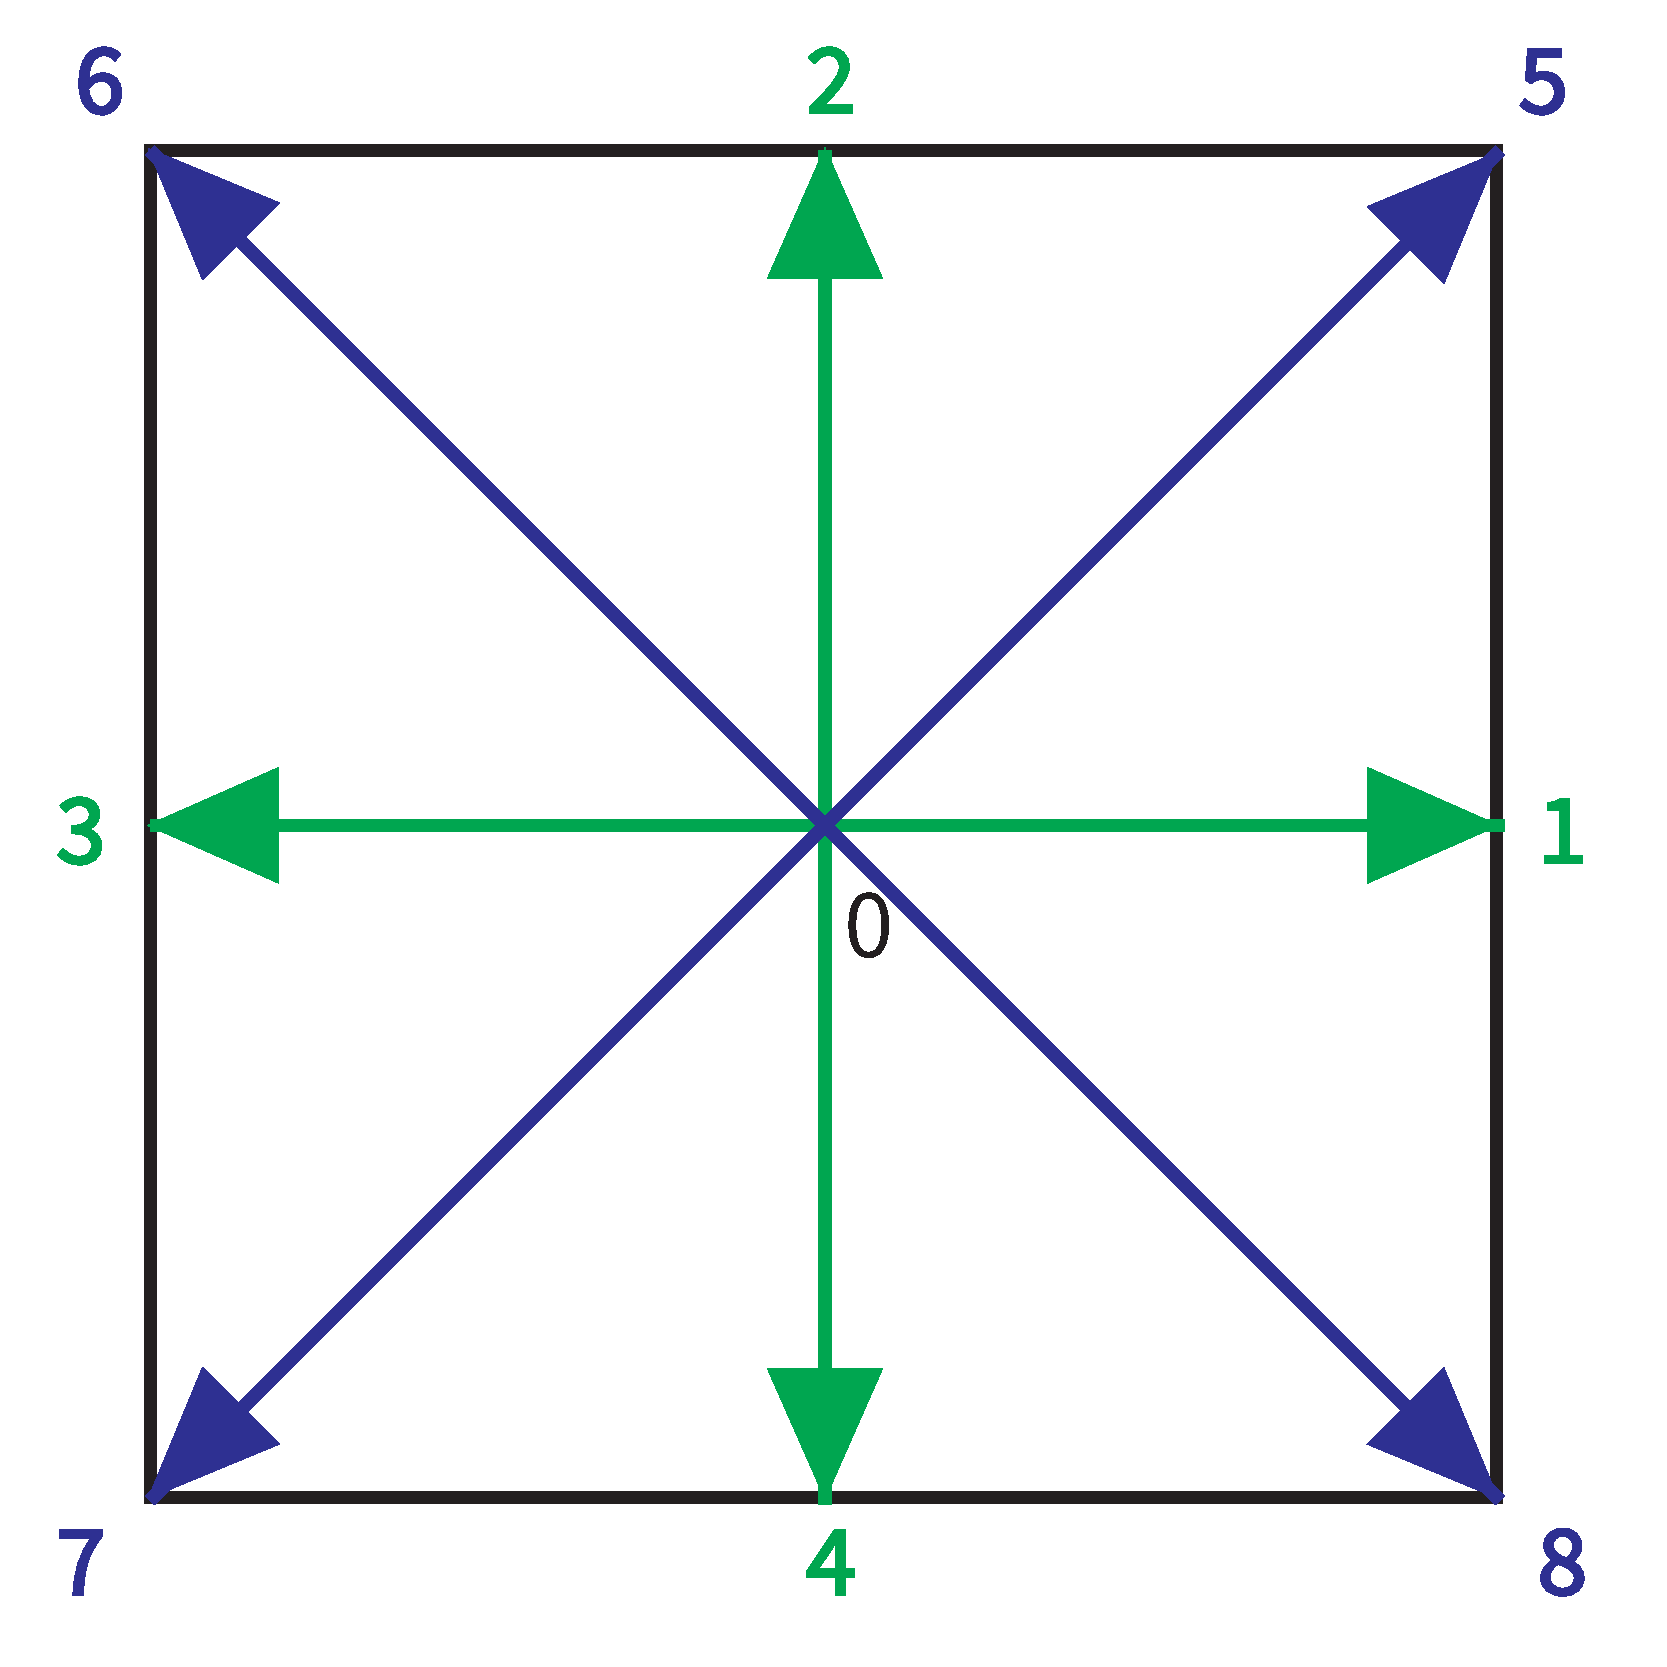
\includegraphics[width=0.3\textwidth]{figures/D2Q9_colored.pdf}%
	} \qquad
	\subfloat[D3Q27.\label{fig:d3q27-node}]{%
		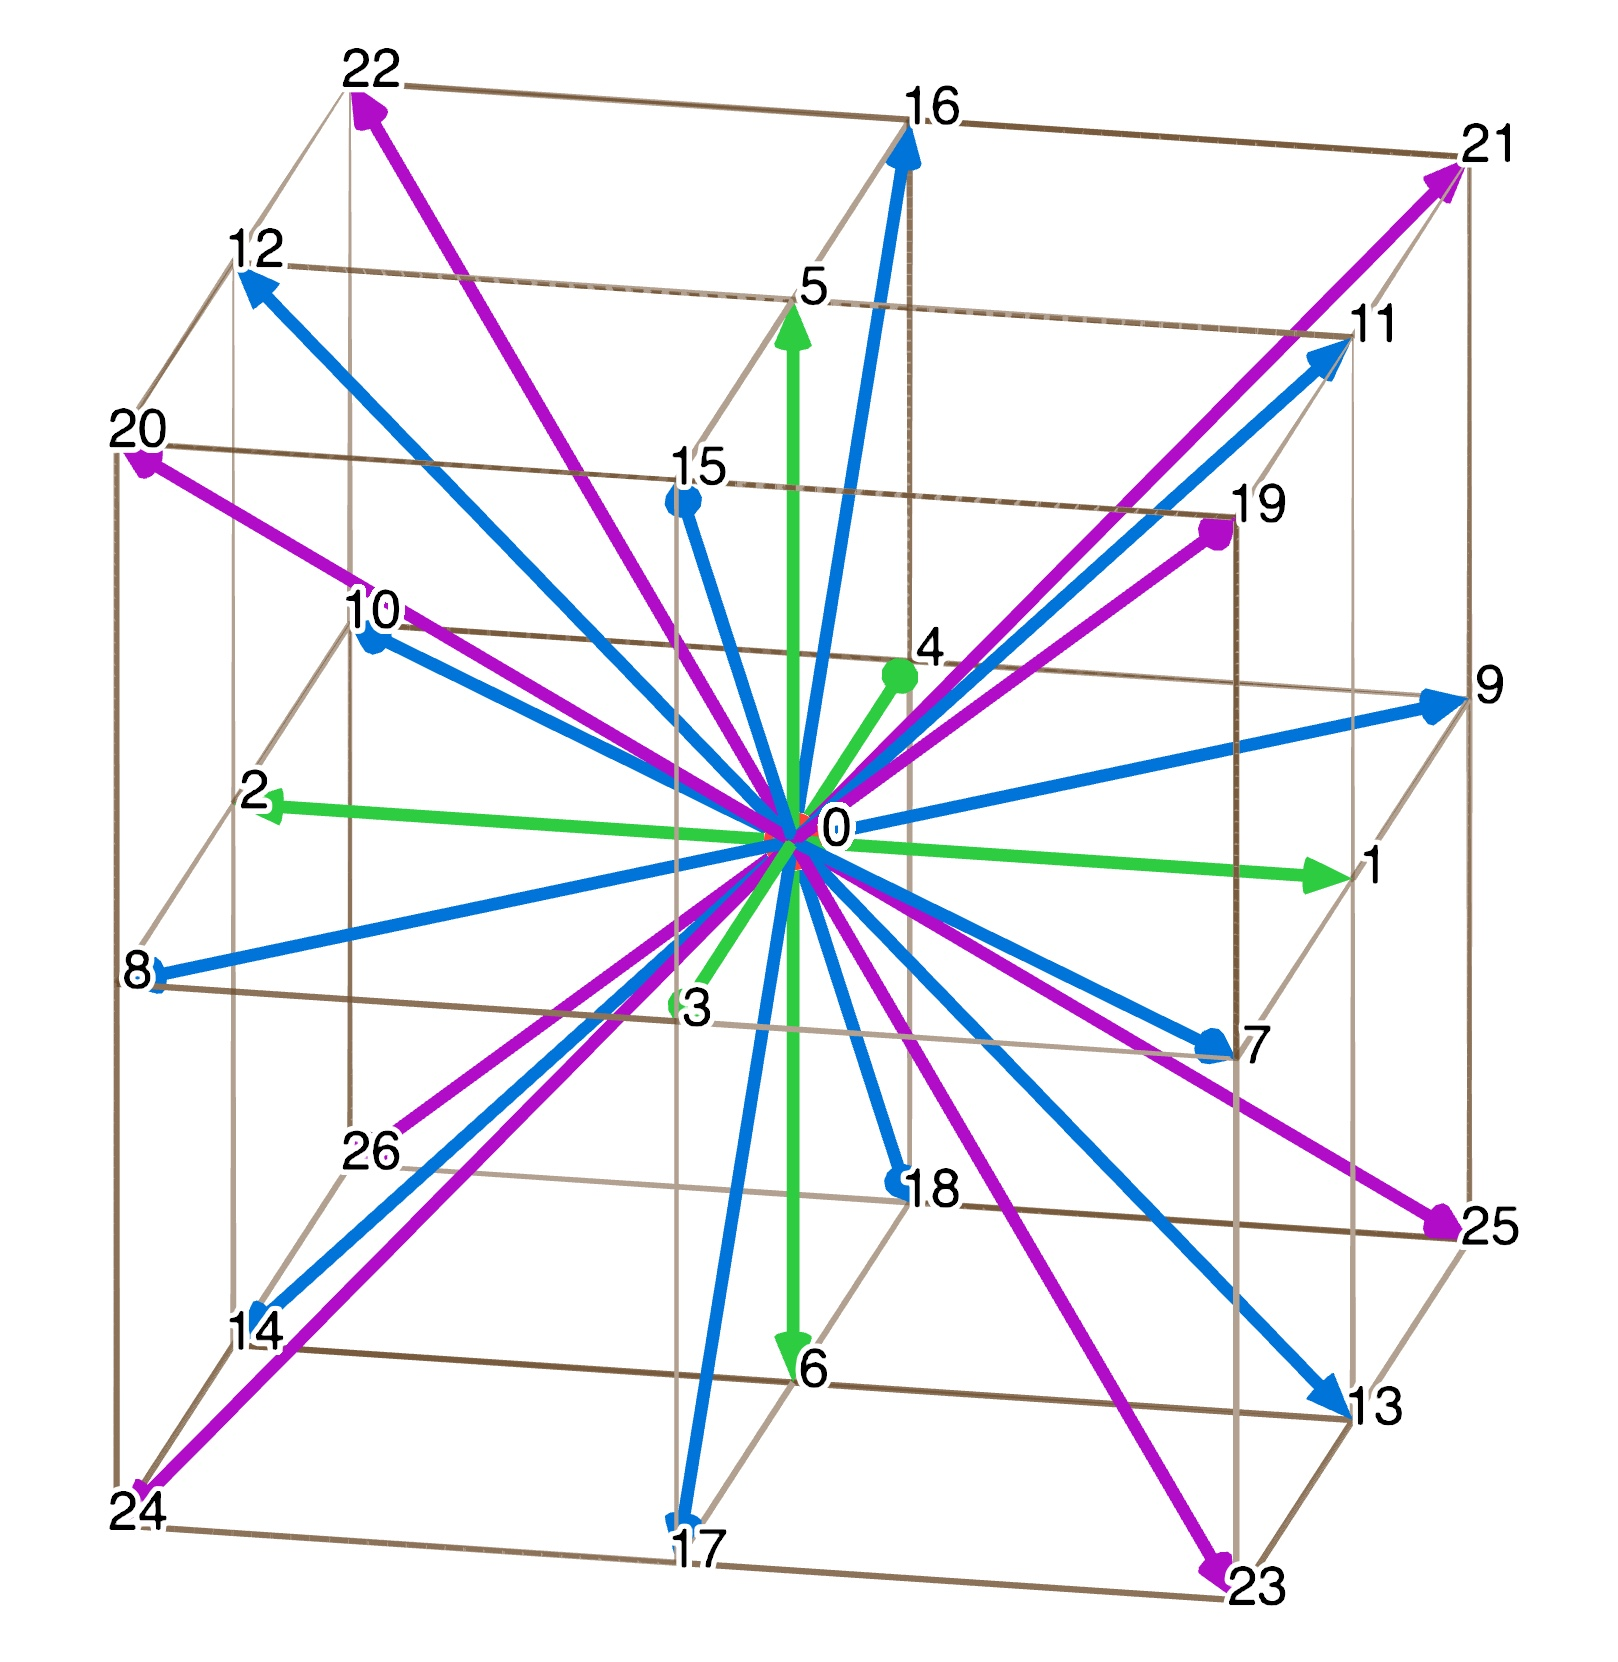
\includegraphics[width=0.32\textwidth]{figures/d3q27.jpg}%
	}
	\caption{Lattice stencils.}
	\label{fig:stencils}
\end{figure}

The LBE can be stated as

\begin{equation}
	\label{eq:lbe-bgk}
	f_i (\bm{x}+\bm{e}_i\Delta t,t+\Delta t) = f_i (\bm{x},t)-\frac{1}{\tau}\Big[f_i (\bm{x},t) - f_i^{eq} (\bm{x},t)\Big],
\end{equation}
where $f_i (\bm{x},t)$ denotes the individual direction of the PDF at each lattice point in particular time and $f_i (\bm{x}+\bm{e}_i\Delta t,t+\Delta t)$ is equal to resulting PDF for all neighbouring nodes in the next iteration step. Necessary criterion for stability is that physical information should not travel faster than fastest speed supported by the lattice \citep{succi2001lattice}. Discrete velocities $\bm{e}_i$ in D2Q9 model can be expressed in an array as

\begin{equation}
	\label{discrete-velocities}
	\bm{e}_i = \begin{bmatrix}
		\phantom{-}0 & \phantom{-}1 & \phantom{-}0 &-1 & \phantom{-}0 & \phantom{-}1 &-1 &-1 & \phantom{-}1\phantom{-}\\
		\phantom{-}0 & \phantom{-}0 & \phantom{-}1 & \phantom{-}0 &-1 & \phantom{-}1 & \phantom{-}1 &-1 &-1\phantom{-}
	\end{bmatrix}
\end{equation}

for the single node in 2D grid and for D3Q27 the array is extended to accommodate 27 velocities moving in 3D grid

\begin{equation}
	\label{discrete-velocities-3d}
	\resizebox{0.89\textwidth}{!}{$\bm{e}_i = \left[ \begin{array}{@{}*{27}{c}@{}}
			\phantom{-}0 & \phantom{-}1 &-1 & \phantom{-}0 & \phantom{-}0 & \phantom{-}0 & \phantom{-}0 & \phantom{-}1 &-1 & \phantom{-}1 &-1 & \phantom{-}1 &-1 & \phantom{-}1 &-1 & \phantom{-}0 & \phantom{-}0 & \phantom{-}0 & \phantom{-}0 & \phantom{-}1&-1 & \phantom{-}1 &-1 & \phantom{-}1 &-1 & \phantom{-}1 &-1 \phantom{-} \\
			\phantom{-}0 & \phantom{-}0 & \phantom{-}0 & \phantom{-}1 &-1 & \phantom{-}0 & \phantom{-}0 & \phantom{-}1 & \phantom{-}1 &-1 &-1 & \phantom{-}0 & \phantom{-}0 & \phantom{-}0 & \phantom{-}0 & \phantom{-}1 &-1 & \phantom{-}1 &-1 & \phantom{-}1 & \phantom{-}1 &-1 &-1 & \phantom{-}1 & \phantom{-}1 &-1 &-1 \phantom{-} \\
			\phantom{-}0 & \phantom{-}0 & \phantom{-}0 & \phantom{-}0 & \phantom{-}0 & \phantom{-}1 &-1 & \phantom{-}0 & \phantom{-}0 & \phantom{-}0 & \phantom{-}0 & \phantom{-}1 & \phantom{-}1 &-1 &-1 & \phantom{-}1 & \phantom{-}1 &-1 &-1 & \phantom{-}1 & \phantom{-}1 & \phantom{-}1 & \phantom{-}1 &-1 &-1 &-1 &-1\phantom{-}
		\end{array} \right]$}
\end{equation}

Macroscopic quantities are obtained from hydrodynamic moments of the distribution function (Eq. \ref{eq:density}, \ref{eq:velocity})

\begin{equation}
	\label{eq:density}
	\rho = \sum_{i=0}^{Q}f_i,
\end{equation}

\begin{equation}
	\label{eq:velocity}
	\rho\bm{u} = \sum_{i=0}^{Q} \bm{e}_i  f_i .
\end{equation}

Equilibrium distribution function $f^{eq}$ can be expressed by performing a Hermite expansion of the Boltzmann equilibrium function as

\begin{equation}
	\label{eq:feq}
	f_i^{eq} = \omega_i \rho \left( 1+3\frac{\bm{e}_i \cdot \bm{u}}{c_s} + \frac{9}{2}\frac{(\bm{e}_i \cdot \bm{u})^2}{c_s^2}-\frac{3}{2}\frac{\bm{u}^2}{c_s^2}\right),
\end{equation}
where $c_s$ is the speed of sound within the lattice, usually set to $c_s = \frac{1}{\sqrt{3}}$ and $\omega$ denotes different weights for discrete velocity in D2Q9 stencil

\begin{align}
	\label{weights}
	\omega_0 &= 4/9,\\
	\omega_{1,2,3,4} &= 1/9,\\
	\omega_{5,6,7,8} &= 1/36.
\end{align}

With a proper set of discrete velocities, the LBE recovers the incompressible Navier–Stokes equations by the Chapman–Enskog expansion. For the flows within the incompressible limit, assumptions such as low-Mach number and variations in density of order $\mathcal{O}(M^2)$ has to be made.

Two general steps of the LBM solver involve solving  Eq. \ref{eq:collision} for collision and Eq. \ref{eq:streaming} for streaming in each iteration.

\begin{equation}
	\label{eq:collision}
	f_i (\bm{x},t+\Delta t) = f_i (\bm{x},t)-\frac{1}{\tau}\Big[f_i (\bm{x},t) - f_i^{eq} (\bm{x},t)\Big].
\end{equation}

\begin{equation}
	\label{eq:streaming}
	f_i (\bm{x}+\bm{e}_i\Delta t,t+\Delta t) = f_i (\bm{x},t+\Delta t).
\end{equation}

To overcome difficulties of numerical instability in applying the 3D LBM method, the multiple-relaxation-time (MRT) scheme is useful to stabilize the solution and to obtain satisfactory results. The MRT model allows for independent tuning of the relaxation times for each physical process \citep{sugaD3Q27MultiplerelaxationtimeLattice2015}. It's therefore natural to extend current work to include MRT. In this study we implemented non-orthogonal MRT-LBM in D3Q27 because it simplifies the transformation between the discrete velocity space and the moment space \citep{feiModelingRealisticMultiphase2019}.

The collision operator in MRT-LBM is defined as 

\begin{equation}
	\Omega_{MRT} = M^{-1} SM,
\end{equation}

where $S$ is a diagonal relaxation matrix and $M$ being the transformation matrix \citep{feiModelingRealisticMultiphase2019}. The collision step is performed in moment space. Formally it can be defined as

\begin{equation}
	m^* = m - S(m-m^{eq}),
\end{equation}

where $m = Mf$ and $m^{eq} = Mf^{eq}$. After the collision step, the distribution function is be reconstructed by $f^* = M^{-1}m^*$ and used in the streaming step as usual

\begin{equation}
	\label{eq:lbe-post-collision}
	f_i (\bm{x}+\bm{e}_i\Delta t,t+\Delta t) = f^{*}_i (\bm{x},t+\Delta t).
\end{equation}

%For the boundary condition, we implemented a simple no-slip boundary known as bounce-back, which effectively reverses the direction of $f_i$ \cite{Mawson2014InteractiveFI}. In places like input and output of simulated pipe for Kármán vortex test case, we implemented periodic boundary conditions \cite{succi2018lattice}.


%\subsection{Kinetic Theory}
%
%% --- move me? + prepisat/dopisat
%The fluid mechanics (and it's subsequent branch of fluid dynamics) work with the inherent continuum assumption, under which fluids are treated as continuous, even though at the microscopic scale they are composed of molecules. Within the continuum assumption, the macroscopic properties such as density, pressure, bulk velocity can be defined as very small (infinitesimal) elements, in molecular length scales such elements would be regarded as very large. The continuum hypothesis is not accurate enough for the problems of molecular or nano-scale flows, or for very high speeds of fluid flows like supersonic flow.
%% ------------------------
%
%The main properties of any numerical scheme can be classified as follows \citep{succi2001lattice}:
%
%\begin{itemize}
%	\item causality,
%	\item accuracy,
%	\item stability,
%	\item consistency,
%	\item efficiency,
%	\item flexibility. 
%\end{itemize}
%
%With respect to above properties, lattice Boltzmann equation (LBE) can be classified as an explicit, Lagrangian, finite-hyperbolicity approximation of Navier-Stokes equations. 
%
%
%The LBE is obtained by discretizing the velocity space of the Boltzmann equation into a finite number of discrete velocities $e_\alpha$ \{$\alpha$ = 0,1,...,26\}. With a proper set of discrete velocities, the LBE recovers the continuum Navier–Stokes equations by the Chapman–Enskog expansion.
%
%
%\begin{figure}[!ht]
%	\centering
%	\subfloat[D3Q19]{{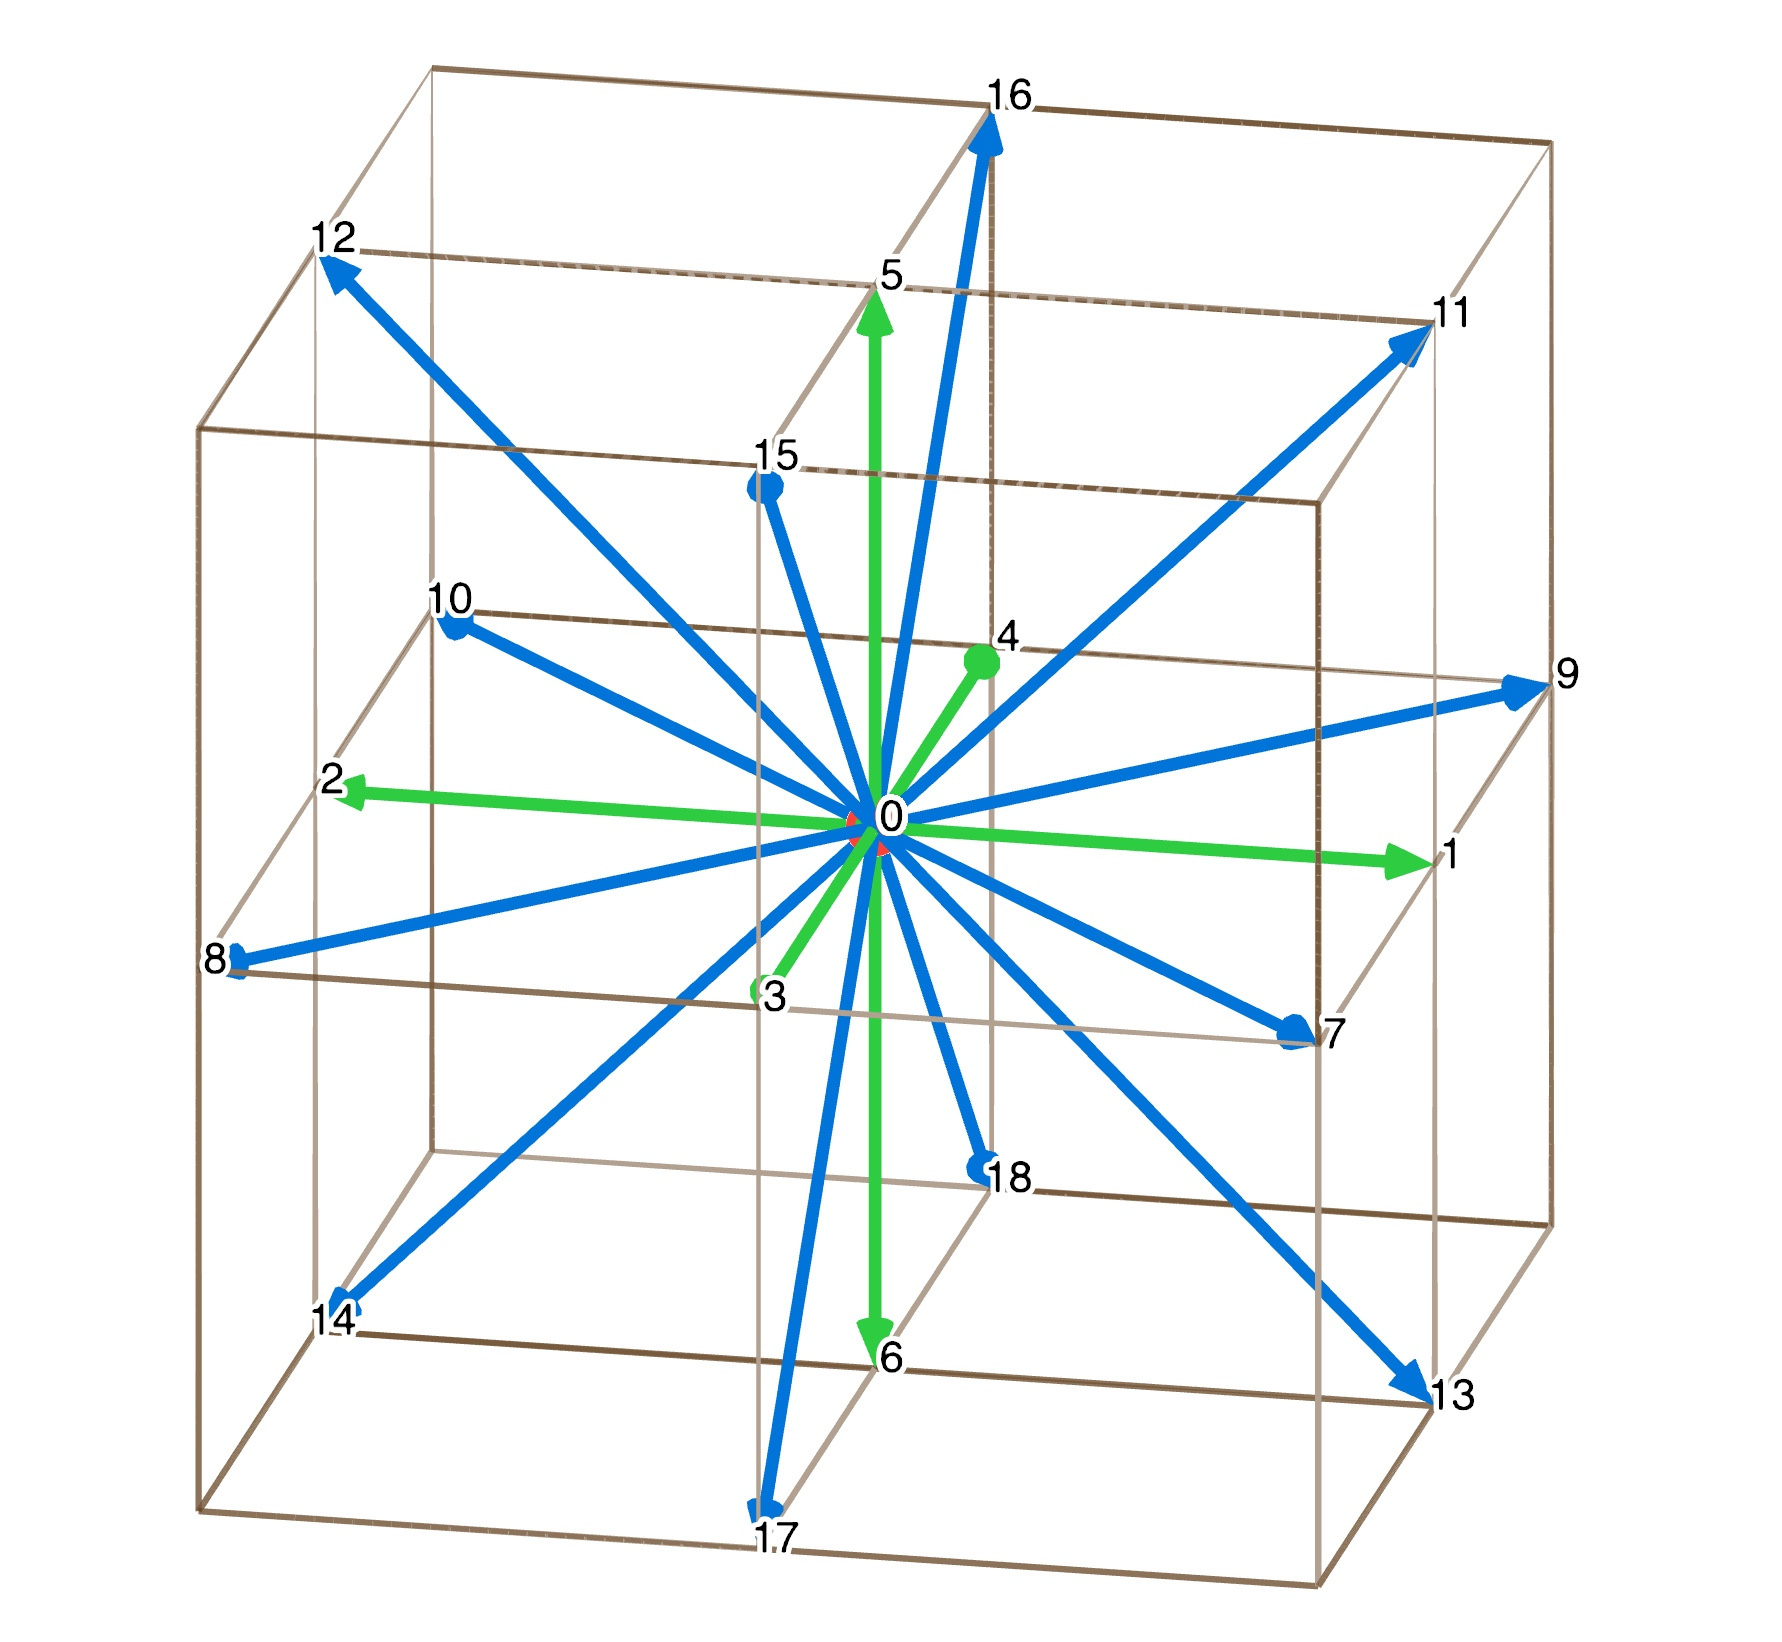
\includegraphics[width=6cm]{figures/d3q19.jpg} }}
%	\qquad
%	\subfloat[D3Q27]{{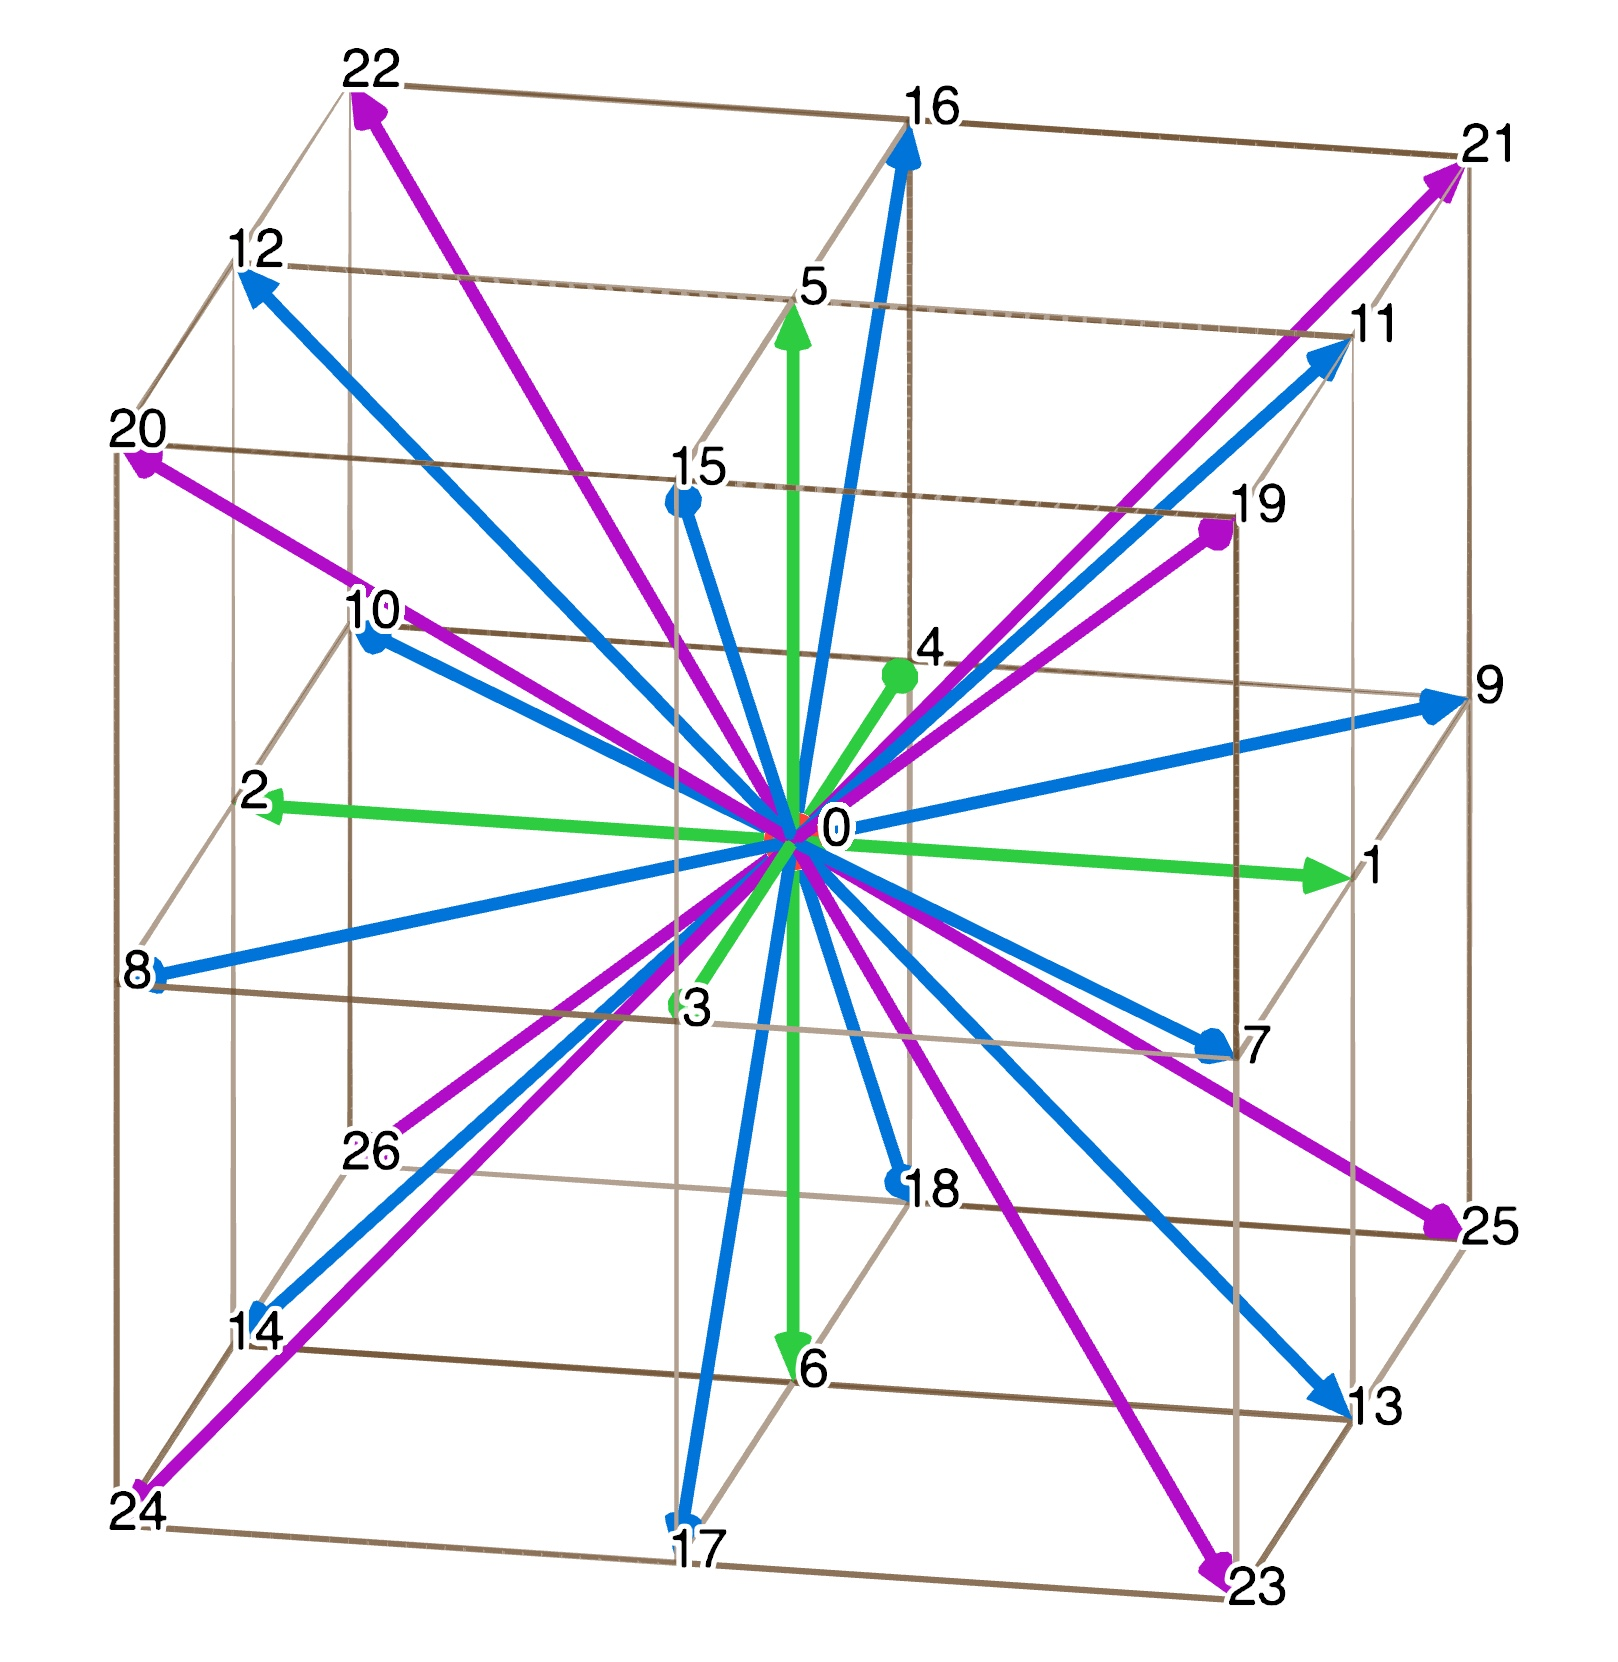
\includegraphics[width=6cm]{figures/d3q27.jpg} }}
%	\caption{Three-dimensional lattice node schemes.}
%	\label{fig:lattice-node-schemes}
%\end{figure}
%
%
%Caution have to be taken when working within lattice's discrete world. For simulating the interface of blown oxygen with melted fluid slag, we're working with higher Mach speeds. The basic notion is that the lattice can only support signals with a finite propagation speed. Necessary criterion for stability is that physical information should not travel faster than fastest speed supported by the lattice \cite{succi2001lattice}.
%
%We can calculate the error to $\varepsilon(Ma^3)$ in space and proportional to $\varepsilon (Ma \cdot dt)$ in time, where $Ma = \frac{u}{c_s}$ is the Mach number of the system.
%
%$p = c_s^2 \rho$ is the pressure, $c_s = \frac{c}{\sqrt{3}}$ is the speed of sound, and the kinematic and viscosity $\nu$ is related to the relaxation time rates for the second-order moments by $\nu = \left(\frac{1}{s_v - 0.5}\right) c_s^2 \Delta t$ and $\xi = \frac{2}{3}\left(\frac{1}{s_b - 0.5}\right)$ respectively.


%\subsection{Bhatnagar-Gross-Krook Model}
%
%
%- TODO: napisat aj o klasickom BGK modeli \citep{bhatnagarModelCollisionProcesses1954}
%
%The collision operator $\Omega$ is difficult to solve. It's been simplified by the work of Bhatnagar, Gross and Crook \cite{bhatnagarModelCollisionProcesses1954}, that introduced the BGK operator
%
%\begin{equation}
%	\label{eq:std-bgk}
%	f_i (\bm{x}+\bm{e}_i\Delta t,t+\Delta t) = f_i (\bm{x},t)-\frac{1}{\tau}\Big(f_i (\bm{x},t) - f_i^{eq} (\bm{x},t)\Big)
%\end{equation}
%
%In the presence of a body force density $\bm{F} = \rho \bm{g}$, where $\bm{g}$ is
%the acceleration due to $\bm{F}$, the LBE must be modified to account for the force \cite{guoDiscreteLatticeEffects2002}.
%
%\begin{equation}
%	\label{eq:feq}
%	f_i^{eq} = \omega_i \rho \left( 1+3\frac{\bm{e}_i \cdot \bm{u}}{c} + \frac{9}{2}\frac{(\bm{e}_i \cdot \bm{u})^2}{c^2}-\frac{3}{2}\frac{\bm{u}^2}{c^2}\right)
%\end{equation}
%
%\begin{equation}
%	\label{eq:density}
%	\rho = \sum_{i=0}^{27}f_i
%\end{equation}
%
%\begin{equation}
%	\label{eq:velocity}
%	\rho\bm{u} = \sum_{i=0}^{27} f_i \bm{e}_i + \frac{\Delta t \bm{F}}{2}
%\end{equation}
%
%\subsection{Multiple Relaxation Time}
%
%% --- Prepisat -------------------
%To overcome difficulties of numerical instability in applying the LBM method, the multiple-relaxation-time (MRT) scheme is useful to stabilize the solution and to obtain satisfactory results because the MRT model allows the usage of an independently optimized relaxation-time for each physical process \cite{sugaD3Q27MultiplerelaxationtimeLattice2015}.
%% -----------------------------------------------
%
%A general collision step in MRT can be written as \cite{feiModelingRealisticMultiphase2019}
%
%\begin{equation}
%	\label{eq:mrt-collision}
%	f_i^{*} (\bm{x},t) = f_i (\bm{x},t)-\Lambda_{i,k}\big[f_k - f_k^{eq}\big]_{(\bm{x},t)} +\frac{\Delta t}{2} \big[ F_i (\bm{x},t) +  F_i (\bm{x}+\bm{e}_i\Delta t,t+\Delta t) \big]
%\end{equation}
%
%where $\bm{x}$ is the spatial position in the 3D grid, $t$ is time, $F_i$ are the forcing terms in discrete velocity space, and collision operator $\Lambda_{i,k}$ computed as \cite{feiModelingRealisticMultiphase2019}
%
%Although many schemes to discretize the velocity space have been proposed, for three-dimensional (3-D) flows, the present study focuses on so called the three- dimensional twenty-seven (D3Q27) discrete velocity model which is illustrated in Figure~ 1. Table 1 lists the sound speed $c_S$ , the discrete velocity $e_\alpha$ and the weight parameter $w_\alpha$ in the model with $c = \delta x / \delta t$ where $\delta x$ and $\delta t$ are the lattice spacing and the time step, respectively. The MRT LBM transforms the distribution function in the velocity space to the moment space by the transformation matrix $M$ . Transformation matrix $\bm{M}$ can be obtained from Eqs. \ref{eq:moments}.
%
%\begin{equation}
%	\label{eq:moments}
%	M = ... doplnit
%\end{equation}
%
%Since the moments of the distribution function correspond directly to flow quantities, the moment representation allows us to perform the relaxation processes with different relaxation-times according to different time-scales of various physical processes. The evolution equation for the particle distribution function f is thus written as
%
%\begin{equation}
%	|f (x_i +e_\alpha \delta t,t+ \delta t)\rangle-|f (x_i,t)\rangle=-M^{-1} S [|m(x_i,t)\rangle - |m^{eq} (x_i,t)\rangle]+|F(x_i,t)\rangle.
%\end{equation}
%
%where $x_i$ is the position vector of node i, $\vec{S}$ is the collision matrix, $m$ is the moment, $F$ represents an external body force and the notation for the column vector (known as the ket vector) such as $|f \rangle$ represents
%
%\begin{equation}
%	\label{eq:collision-operator-mrt}
%	\Lambda_{i,k} = (\bm{M}^{-1}\bm{SM})_{i,k}
%\end{equation}
%
%in which $S$ is a diagonal relaxation matrix.
%
%\begin{equation}
%	\label{eq:feq}
%	f_i^{eq} = \omega_i \rho \left( 1+3\frac{\bm{e}_i \cdot \bm{u}}{c} + \frac{9}{2}\frac{(\bm{e}_i \cdot \bm{u})^2}{c^2}-\frac{3}{2}\frac{\bm{u}^2}{c^2}\right)
%\end{equation}
%
%
%\begin{equation}
%	\label{eq:collision-moment-space}
%	\small
%	\bm{m^*}=\bm{m}-\bm{S}\big(\bm{m}-\bm{m}^{eq}\big)+\Big(\bm{I}-\frac{\bm{S}}{2}\Big)\Delta t\bm{F}
%\end{equation}
%
%where $\bm{m}=\bm{Mf}$, $\bm{m^{eq}}=\bm{Mf^{eq}}$, and $\bm{F}=\bm{MF}$.
%
%%\begin{equation}
%%|f (x_i,t)\rangle = (f_0(x_i,t),f_1(x_i,t),...,f_Q−1(x_i,t)).
%%\end{equation}
%
%\begin{equation}
%	\label{eq:moments}
%	\bm{m} = [m_0, m_1,...,m_{26}]^T
%\end{equation}
%
%For better numerical stability, Multiple Relaxation Time (MRT) scheme is used. It allows for more degrees of freedom and better tunability of relaxation parameters. Stability is a key property in any numerical scheme \cite{succi2001lattice}. It helps to protect against cumulative error build-up or other sources of inaccuracies.


\subsection{Boundary Conditions}
%DONE
Dynamics of the fluid flow is dependent on the surrounding environment described mathematically with suitable boundary conditions. They play a crucial role as they select solutions which are compatible with external constraints. Their overall treatment makes the difference in the quality of CFD simulation \citep{succi2018}.

At the start point during the simulation initialization phase, an initial conditions have to be set up. They are basically a boundary conditions at $t = 0$. Popular practice is to set the PDF to local equilibrium according to the prescribed value of the hydrodynamic field and initial density with initial velocity to zero

\begin{equation}
	\label{eq:initial-conditions-pdf}
	f_i (\bm{x},t_0) = f_i^{eq} (\bm{x},t_0),
\end{equation}

\begin{equation}
	\label{eq:initial-conditions-density}
	\rho_0 (\bm{x}) = \rho (\bm{x},t_0), 
\end{equation}

\begin{equation}
	\label{eq:initial-conditions-velocity}
	\bm{u}_0 (\bm{x}) = \bm{u} (\bm{x},t_0).
\end{equation}

Geometric boundary conditions have multiple forms, namely:

\begin{itemize}
	\item periodic,
	\item no-slip,
	\item free-slip,
	\item frictional slip,
	\item sliding walls,
	\item open inlet and outlet.
\end{itemize}

Various LBM solvers implement different types of listed boundary conditions, but usually for the sake of simplicity and lower computational cost, periodic and no-slip are used. Periodic boundary conditions are one of the simplest to implement. They are typically used to isolate bulk fluid phenomena from boundaries of physical system. No-slip boundary-condition, also known as bounce-back, refers to solid surfaces with zero fluid velocities. They expect that the solid walls have enough rugosity to prevent any additional motion of the fluid relative to the wall \citep{succi2018}. Effectively, this results in a reversal of the discrete velocities direction of $f_i$ \citep{Mawson2014InteractiveFI}.

In current work, the simulation software implements a simple no-slip boundary. In places like inflow and outflow of simulated pipe for Kármán vortex test case, we implemented periodic boundary conditions \citep{succi2001lattice}.
% --------------------------

%
%\subsection{Turbulence Modeling}
%
%
%\subsubsection{Fluid Turbulence}
%
%% upravit (z https://www.math.u-bordeaux.fr/~marnaudo/publis/Text_Fig3_f.pdf)
%Turbulent regimes are often studied in the perspective of the theory of dynamical systems as chaotic systems, which are characterized by a strong sensitivity to
%initial conditions.
%
%Simple regular Euler flow can give rise to chaotic particle trajectories, a phenomenon which has been intensively studied, is also present in fluid dynamics ..
%
%turbulence modelling using the Smagorinsky model in LBM for the simulation of high Reynolds number flow and the coupling of two LBM simulations to simulate thermal flows under the Boussinesq approximation.
%
%\subsubsection{Sub-grid Scale Modeling}

\subsection{Multiphase Flows}
% DONE
An important area of LBM applications is multiphase and multicomponent simulations. Such phenomena can be observed when fluids of different densities meet at some interface, usually between gases and liquids. A deeper understanding of the fundamental physics of such complex interfaces is of great importance in many natural and industrial processes. 

Dynamics of multicomponent flows are difficult to investigate due to thinness and complexness of the interface between them. The problem with multiphase flows, in turn, can be very short times of change between phases. Additionally, the density ratio and Weber and Reynolds numbers involved in many practical multiphase flows, such as binary droplet collisions and melt-jet breakup, are usually very high, which further increases the complexity of the phenomena involved \citep{feiModelingRealisticMultiphase2019}. 

Development of accurate and robust multiphase models to investigate complex processes at the interfaces is crucial. Such models mostly fall into the following categories:

\begin{itemize}
	\item color-gradient methods,
	\item pseudopotential methods,
	\item free-energy methods,
	\item phase-field methods.
\end{itemize}

All of aforementioned methods were successfully applied to dynamic multiphase flows at large density ratios ($\rho_l / \rho_g \approx 10^3$) and high Reynolds numbers \citep{liLatticeBoltzmannMethods2016a}. Practical applications include droplet splashing and droplet collision, water-gas two-phase transport in fuel cells, electrolyte transport dynamics in batteries, and phase-change heat transfer like boiling or evaporation.

Although multiphase flows are interesting use-case for LBM simulation, their support was not implemented in current solver implementation described in this thesis. But at the same time, some parts of the research that is being done at the Institute of Control and Informatization of Production Processes at Technical University of Košice, where I currently work, focuses on steelmaking and underground gasification of coal. Simulating involved processes with LBM and multiphase methods can pave a new way towards better understanding of the phenomena in those areas.

%% --- Prepisat -------------------
%Interfaces between different phases and/or components are ubiquitous in multiphase flows and energy applications, such as rain dynamics, plant spraying, water boiling, and gas turbine blade cooling, to name but a few. A deeper understanding of the fundamental physics of such complex interfaces is of great importance in many natural and industrial processes. The dynamics of the interfaces is difficult to investigate because typical interfaces are extremely thin, complex in shape, and deforming at short time scales. In addition, the density ratio and Weber and Reynolds numbers involved in many practical multiphase flows, such as binary droplet collisions and melt-jet breakup, are usually very high, which further increases the complexity of the phenomena involved. Therefore, development of robust and accurate computational methods to capture the complex interfacial phenomena is crucial in the study of multiphase flows \cite{feiModelingRealisticMultiphase2019}.
%% -----------------------------------
%
%% prepisat
%Non-ideal fluids and multiphase flows. 
%A major area of LB application is the simulation of a variety of multiphase and multicomponent flows [24–26]. Here, the main asset is the flexibility of the source term and/or local equilibria towards the inclusion of non-ideal interactions. A particularly popular expression is the one proposed by Shan and Chen,
%
%\begin{equation}
%	\vec{F}(\vec{x}) = \psi(\vec{x}) \sum_{i=0}^{b}G(\vec{x},\vec{x}+\vec{c_i})\vec{c_i}\psi(\vec{x}+\vec{c_i}),
%\end{equation}
%
%where $\psi(\vec{x})$ is a local functional of the fluid density $\rho(\vec{x})$.
%
%By proper choice of this functional, the main features of non-ideal fluids, namely a non-monotonic equation of state supporting phase transitions and non-zero surface tension can be incorporated at a minimum programming effort. This simple variant opens up a vast scenario of applications involving multiphase and multicomponent flows, including foams and emulsions (see Figure~ 2). Needless to say, this variant comes with a number of limitations, such as fake interface currents, which severly constrain the accessible range of density ratios between the liquid and vapor phase. Yet, owing to its simplicity and efficiency, the method has gained increasing popularity over the years. Subsequent developments have improved significantly over the original version, but much remains to be done to gain further accuracy, especially in terms of multigrid/multiscale procedures at complex fluid interfaces. Another important issue is the incorporation of finite-temperature fluctuations for nanoscale flows.
%
%% dopisat
%existing multiphase LB models can be classified into four categories: the color-gradient model, the pseudopotential model, the it was shown by Li et al. that a non-orthogonal MRT-LBM free-energy model, and the mean-field model.
%%
%
%% --- Prepisat -------------------
%Among them, can retain the numerical accuracy while simplifying the implementation of its orthogonal counterpart. In parallel, the CLBM which can be viewed as a non-orthogonal MRT-LBM in the co-moving frame, has been shown to possess very good numerical stability for high Rayleigh number thermal flows,39 as well the pseudopotential model is considered in the present work due to its simplicity and computational efficiency. In this model, the interactions among populations of molecules are modeled by a density-dependent pseudopotential. Through interactions among the particles on the nearest-neighboring sites, phase separation and breakup and/or merging of phase interfaces can be achieved automatically. For further details about the multiphase LB models, interested readers are directed to some comprehensive review
%% ------------------------------------


\subsection{Adaptive Mesh Refinement}
% DONE?
Turbulent flows or multiphase flows involves different densities, like gas bubbles, liquid droplets or creation of foam. Turbulence is a complex, non-linear, multi-scale phenomenon, which is very difficult to simulate accurately for smaller parts of the turbulent flows. Problem with bubbles is that the gas-liquid interface typically spans to a thickness of 3-5 grid spacing. Both of these problems need denser grid to accurately represent them, thus requiring more computational power to simulate them effectively. Typically, not everything in the computational domain needs to be represented with the same amount of accuracy.

Effective technique for such problems can be an Adaptive Mesh Refinement. With this technique, the mesh resolution is not constant, but adapts according to the accuracy requirements in specific part of the domain. Fine mesh resolution is used for problematic parts where high accuracy is needed and coarse mesh is applied to the bulk fluid away from the interface. This gives a tremendous benefit in reducing the computation cost \citep{yuanAdaptiveMeshRefinementmultiphase2017}.

\subsection{Complex Fluids and Beyond}
% DONE
In modern science and technology, we often deal with complex flows such as flows with chemical reactions, phase transitions, suspended particles, etc. Broad range of physical phenomena go beyond the classic Navier-Stokes equations. For instance, it's possible to implement a electromagnetic forces within the Lattice-Boltzmann formalism, opening the door to magnetohydrodynamics. As a result, this allows extending LBM to be used for studying properties and dynamics of plasmas, liquid metals, salt water or electrolytes.

Another interesting frontier of modern physics is soft matter, in which LBM is also trying to establish itself as a viable method for studying polymers, foams, gels, granular materials, liquid crystals and some biological materials.

It doesn't stay there. Lattice-Boltzmann formalism doesn't restrict itself only to classical Newtonian mechanics, but allows to be extended to the case of relativistic as well as quantum fluids in a comparatively simple manner. The kinetic theory harnessed in LBM can serve as a very effective functional generator of a variety of linear and non-linear partial differential equations of mathematical physics \citep{succi2018}.

% -------------------------------------------------------------------------------

\section{GPU Computing}
\label{gpu-computing}
% DONE
Innovations in GPUs over the last decades was driven mainly by video games. They advanced from merely displaying pixels to being capable of doing mathematical computations. After the introduction of programmable shaders and floating-point support on graphics processors, the dynamics has changed though. At first it opened the door for using GPUs in complex physics calculations like wind blowing, fluid flows, cloth movement, etc. in games but also for scientific simulation. This movement to leveraging GPU capabilities in serious engineering work became dubbed as general-purpose computing on GPUs (GPGPU), a term coined by NVIDIA's Distinguished Engineer Mark Harris.

GPU-based parallel computing reduces the time for heavy computation tasks like training a machine learning system on large data set, climate modeling, protein folding, drug discovery, or data analysis, by orders of magnitude \citep{stortiCUDAEngineersIntroduction2016, PACHECO20111}. The massive parallelism achievable with GPUs pushed the developers to invest more time in creating programs that could use it for their advantage. These gains can be achieved at very reasonable costs in terms of both developer effort and the hardware required. It's now possible to speed-up scientific computations in a way that what took minutes or hours can now be done in seconds or even milliseconds. Although, more computationally intensive tasks like Monte Carlo simulations of molecular dynamics are still hard to speed up to an order of real-time simulation.

Interesting case of engineering problem for which GPU computing is showing tremendous potential is solving differential equations while changing the initial or boundary conditions in real-time. In following sections, various techniques on how to tap into the power of GPU computing will be presented.

\subsection{Parallel Programming}
% DONE
For a long time, performance of computers was determined by the amount of transistors that could be fitted to a dense integrated circuit. By following the Moore's law, software developers could just wait for a predictable increase in transistors count. As speed of transistors increased, their power consumption also increased. This power is dissipated as heat, which poises a problem with reliability of the integrated circuit when it gets too hot. And with transistors getting smaller, packing more of them together makes it approach the limits of integrated circuit's ability to dissipate heat.

Rather then building more complex monolithic processors, the industry has decided to put many simpler processors on a single chip, which becoming multicore processors \citep{PACHECO20111}. Nowadays practically all processor have multiple cores. Unfortunately, most conventional programs were written for single-core systems that couldn't exploit the multiple cores. To effectively use them, software have to employ parallel programming model.

We can consider matrix multiplication as a great exercise to showcase how code can be transformed from serial to parallel programming and differences between CPU and GPU implementation. Lets consider the problem of computing the product of two large, $N \times N$, dense matrices (represented in row-major order). The naive CPU algorithm can look like in Alg. \ref{serial-loop}.

\begin{lstlisting}[language=Cpp, caption=Pseudocode with serial loop., label=serial-loop]
	for (i=0;i<N;i++) {
		for (j=0;j<N;j++) {
			C[i,j] = 0;
			for (k=0;k<N;k++) {
				C[i,j] += A[i,k]*B[k,j];
			}
		}
	}
\end{lstlisting}

This example suffers from poor locality. Elements of $B$ are accessed column-wise and therefore they are not in sequential order in memory. The row $i$ could be removed from cache by the time the inner-most loop of $j$ completes. 

We can write a program that executes on the GPU, which computes the matrix multiplication in a single pass. GPU texture will store $2 \times 2$ blocks of matrix in 4-component texels. The program will read 2 rows from matrix $A$ and 2 columns of $B$ to compute 4 elements of the output matrix $C$ at once (Alg. \ref{parallel-loop}).

\begin{lstlisting}[language=Cpp, caption=Pseudocode with serial loop., label=parallel-loop]
	for (k=0;k<N/2;k++) {
		C[i,j].xyzw += A[i,k].xxzz*B[k,j].xyxy + A[i,k].yyww*B[k,j].zwzw;
	}
\end{lstlisting}

Considering the small size of this toy problem, the difference between CPU and GPU version in computation speed won't be noticeable. But with larger problems in terms of bigger and complex physics simulations, amount of operations can grow to extreme numbers. At that stage, speed differences between slower CPU and faster GPU computation can reach orders of hundreds.

In this work we compared benchmarks of simulation software, developed with parallel algorithms, on CPU and different GPUs. Performance analysis is described in section \ref{perf-analysis}, showing noticeable differences.

%When we talk about parallel programming, we have to distinguish between CPU and GPU parallel programming.
%
%When it comes to heavy computation, leveraging multiple cores that are nowadays ubiquitous in processing units or other hardware accelerators is necessary for achieving better performance.
%
%Quickly skim through: \\
%Distributed memory parallelism \\
%shared memory parallelism \\
%Message-passing, MPI, Pthreads, OpenMP \\
%Rust multithreading with memory-safety guarantees (Rc, Arc)
%
%Venovat sa skor GPU parallelism \\
%Ako maju GPU rozlozenu memory a ako pracuju s threads vseobecne\\
%
%
%% prepisat a doplnit do textu hore?
%Algorithm is bandwidth limited with poor performance and low efficiency (time spent computation versus loading data).



\subsection{Heterogeneous Computing}
% DONE
Scaling of the computational power in high-performance accelerators and supercomputers was historically done by adding more and more CPUs together to a multi-processor distributed system, also known as many-core system. When single CPU started to have multiple cores, scaling the power of those systems was done by switching older CPUs to multi-core ones. But adding more and more cores is not infinite process. With increasing number of transistors stuffed into the same size of the chip, the power and heat starts to rise again. Physical limitations were starting to manifest themselves.

More than a decade ago, the GPUs were starting to supplement CPUs for computational work. The general processor (the CPU) with one type of architecture was being helped by the other processor with different architecture type (the GPU). This was the start of moving from homogenous computing towards heterogeneous computing, for which the coordination of two or more different processors is needed. 

\subsection{CUDA}
%DONE
CUDA is a proprietary hardware and software platform for parallel computing on GPUs created by NVIDIA. It provides access to hardware-specific capabilities of graphics cards equipped with CUDA-enabled graphics processing units \cite{stortiCUDAEngineersIntroduction2016}. The software platform provides a development kit (SDK) and application programming interface (API), build as a superset of C programming language. Since its launch it became a dominant proprietary framework for programming NVIDIA GPUs.

The GPU-based approach to massively parallel computing used by CUDA is also the core technology used in many of the world’s fastest and most energy-efficient supercomputers. The key criterion has evolved from FLOPS (floating point operations per second) to FLOPS/watt (i.e., the ratio of computing productivity to energy consumption), and GPU-based parallelism competes well in terms of FLOPS/watt \citep{stortiCUDAEngineersIntroduction2016}.

\begin{figure}[!ht]
	\centering
	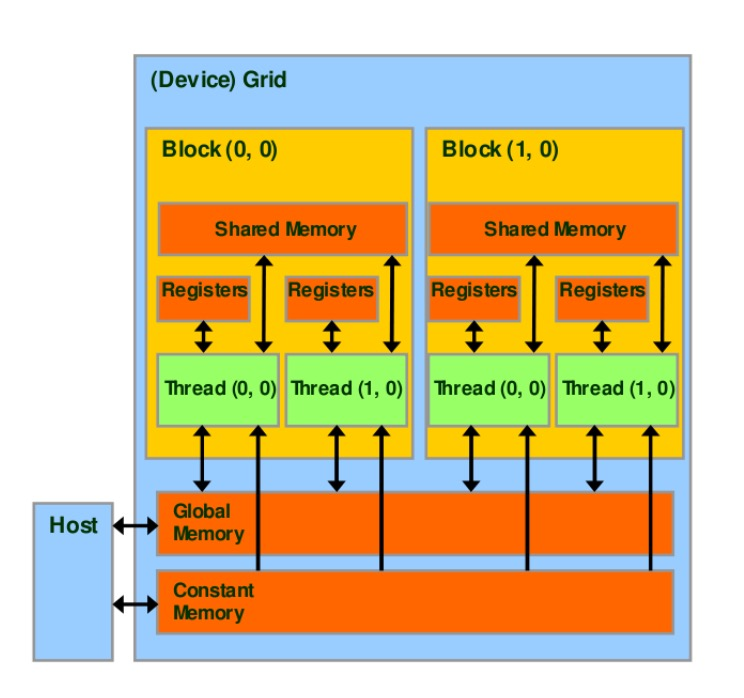
\includegraphics[width=0.5\textwidth]{figures/cuda-device-memory.jpg}
	\caption{CUDA memory model}
	\label{fig:cuda-memory-model}
\end{figure}

\subsection{OpenCL}
% mozno staci
OpenCL (Open Computing Language) is a free and open-source standard for cross-platform, parallel programming of diverse accelerators like CPUs, GPUs, FPGAs, TPUs, etc. found in devices like personal computers or smartphones, embedded platforms, but also high-performance computing systems and supercomputers. In contrast to proprietary nature of CUDA, OpenCL is not tied to any specific hardware manufacturer, which makes its application good for plethora of different hardware.

\subsection{Cross-platform GPU Programming}
\label{sec:computer-simulations-using-gpus}

Despite the growing list of success stories, GPU software development adoption has had a slow rise. The slowness of the rise is attributable to the difficulty in programming GPUs \citep{malcolmArrayFireGPUAcceleration2012a}.

\citep{karimiPerformanceComparisonCUDAa}

CUDA and OpenCL APIs differ from each other. They can be considered as extensions of the C/C++ language and require significant experience in low-level C/C++ programming. To write optimized, parallel software, developers need to employ different techniques, specific to the API they choose, which adds substantial overhead when trying to port one to another in case of a need. In heterogeneous computing systems, trying to write optimized cross-platform code for different GPUs means writing multiple hardware-specific kernels in CUDA and OpenCL.

In this work, a high-performance, parallel computing library ArrayFire has been used to significantly simplify programming for GPUs. Its easy-to-use API provides high-level abstractions in the form of hundreds of functions. They are automatically converted to optimized, fast GPU kernels, utilizing just-in-time (JIT) compilation and lazy evaluation \cite{chrzeszczykMatrixComputationsGPUb}. ArrayFire's high-level object construct called Array is a data structure that acts as a container that represents memory stored on the device. On top of it, ArrayFire provides abstractions in the form of Unified Backend for working with different computational backends. This way it is possible to switch to CPU, GPU, FPGA, or another type of accelerator at runtime \cite{Yalamanchili2015} (Alg. \ref{cpp-backends}), and permits programmers to write massively parallel applications in a high-level language with a much lower number of lines of code (LoC). Arrays (or matrices) of up to 4 dimensions can be created. 

\begin{lstlisting}[language=Cpp, caption=C++ code for setting different computing backends., label=cpp-backends]
	#include <arrayfire.h>
	int main()
	{
		af::setBackend(AF_BACKEND_CUDA);
		// af::setBackend(AF_BACKEND_OPENCL);
		// af::setBackend(AF_BACKEND_CPU);
		return 0;
	}
\end{lstlisting}

% prepisat (z https://arrayfire.org/arrayfire-rust/book/opencl-interop.html a https://arrayfire.org/arrayfire-rust/book/cuda-interop.html)
Although ArrayFire is quite extensive, there remain many cases in which you may want to write custom kernels in CUDA or OpenCL. For example, you may wish to add ArrayFire to an existing code base to increase your productivity, or you may need to supplement ArrayFire's functionality with your own custom implementation of specific algorithms.

Since I'm targeting different types of GPUs in current work, I'll add examples of how to do the interoperability with OpenCL only. Working with CUDA looks similar in principle, but differs in API implementation (different naming conventions, slightly different semantics when launching kernels).
% zaclenit do textu hore
ArrayFire manages its own context, queue, memory, and creates custom IDs for devices. As such, most of the interoperability functions focus on reducing potential synchronization conflicts between ArrayFire and OpenCL. There is some bookkeeping that needs to be done to integrate custom OpenCL kernel. If your kernels can share operate in the same queue as ArrayFire, you should:

\begin{enumerate}
\item obtain the OpenCL context, device, and queue used by ArrayFire,
\item obtain \texttt{cl_mem} references to Array objects,
\item load, build, and use your kernels,
\item return control of Array memory to ArrayFire.
\end{enumerate}

Note, ArrayFire uses an in-order queue, thus when ArrayFire and your kernels are operating in the same queue, there is no need to perform any synchronization operations.

If your kernels needs to operate in their own OpenCL queue, the process is essentially identical, except you need to instruct ArrayFire to complete its computations using the sync function prior to launching your own kernel and ensure your kernels are complete using clFinish (or similar) commands prior to returning control of the memory to ArrayFire:

\begin{enumerate}
\item obtain the OpenCL context, device, and queue used by ArrayFire,
\item obtain cl_mem references to Array objects,
\item instruct ArrayFire to finish operations using sync,
\item load, build, and use your kernels,
\item instruct OpenCL to finish operations using \texttt{clFinish()} or similar commands,
\item return control of Array memory to ArrayFire.
\end{enumerate}

Adding ArrayFire to an existing application is slightly more involved and can be somewhat tricky due to several optimizations we implement. The most important are as follows:

\begin{itemize}
\item ArrayFire assumes control of all memory provided to it.
\item ArrayFire does not (in general) support in-place memory transactions.
\end{itemize}

To add ArrayFire to existing code you need to:

\begin{enumerate}
\item instruct OpenCL to complete its operations using clFinish (or similar),
\item instruct ArrayFire to use the user-created OpenCL Context,
\item create ArrayFire arrays from OpenCL memory objects,
\item perform ArrayFire operations on the Arrays,
\item instruct ArrayFire to finish operations using sync,
\item obtain \texttt{cl_mem} references for important memory,
\item continue your OpenCL application.
\end{enumerate}
	
ArrayFire's memory manager automatically assumes responsibility for any memory provided to it. If you are creating an array from another RAII style object, you should retain it to ensure your memory is not deallocated if your RAII object were to go out of scope.

If you do not wish for ArrayFire to manage your memory, you may call the \texttt{Array::unlock()} function and manage the memory yourself; however, if you do so, please be cautious not to call \texttt{clReleaseMemObj} on a \texttt{cl_mem} when ArrayFire might be using it!

It is fairly straightforward to interface ArrayFire with your own custom code. ArrayFire provides several functions to ease this process. The pointer returned by \texttt{Array::device_ptr()} should be cast to \texttt{cl_mem} before using it with OpenCL opaque types. The pointer is a \texttt{cl_mem} internally that is force casted to pointer type by ArrayFire before returning the value to caller.

Additionally, the OpenCL backend permits the programmer to add and remove custom devices from the ArrayFire device manager (Table \ref{table:afcl}). These permit you to attach ArrayFire directly to the OpenCL queue used by other portions of your application.

\begin{table}[h!]
	\centering\small
	{\renewcommand{\arraystretch}{1.1}%
		{\setlength{\tabcolsep}{0.4em}
	\begin{tabular}{|c|c|} 
		\hline
		Function & Purpose \\
		\hline
		\texttt{add_device_context} & Add a new device to ArrayFire's device manager \\ 
		\hline
		\texttt{set_device_context} & Set ArrayFire's device from \texttt{cl_device_id} \& \texttt{cl_context} \\
		\hline
		\texttt{delete_device_context} & Remove a device from ArrayFire's device manager \\
		\hline
	\end{tabular}}}
	\caption{Functions for working with OpenCL context in ArrayFire-OpenCL interoperability scenario.}
	\label{table:afcl}
\end{table}

\subsection{Accelerating Lattice Boltzmann Simulations with GPUs}

% done
Nowadays, the limiting factor is the cost of accessing data. It must be watched carefully in LBM applications, because it's going to be more and more demanding as the size of the problems to be simulated increases. A common LBM simulation program needs roughly 200 FLOPS per node and requires about 20 arrays. The amount of Bytes to be accessed in memory for one floating-point operation is in the order of 0.5 Bytes/FLOP. 

% done
To reduce the amount of GPU memory accesses, the data is loaded into extremely fast memory called \emph{cache} that is designed to keep up with the CPU. Useful simulations need large amounts of data to be processed, but loading all of them into cache is impossible as they tend to be limited to few Megabytes. Lattice's computational domain is usually represented by 2D or 3D grid of nodes, each carrying multiple data. Computer memory is one dimensional, which means that the element of 3D array of size $N^3$ lies $4 \times N^2$ bytes away from physically contiguous element. If we consider $x$, $y$ and $z$ axis of 3D domain, it is fine when searching for neighboring nodes in $x$ direction, which, as an innermost index, runs first. But searching for neighbors in $z$ direction for element $f(x,y,z+1)$ means that the distance in 1D memory (called \emph{stride}) would be large. To be able to quickly load such neighbor in $z$ direction, we would need to have whole stride loaded in cache, which would require tens of Megabytes for large simulations of $N \sim 1000$. Optimizing memory access is one of the most critical issues in accelerating large-scale LBM simulations.

Developers have to be careful with the memory limitations, even though GPUs provide high memory bandwidth, as LBM algorithms tend to consume large amounts of memory for storing the data. GPU architecture is designed for high data throughput thanks to the combination of Single Instruction, Multiple Data (SIMD) execution model and multithreading, called Single Instruction, Multiple Threads (SIMT). With the parallel nature of the LBM algorithm, CFD simulations that use it can achieve high speeds not just on HPC systems but also PC workstations with a single GPU. For applications of real-time or online interactive visualization of the running simulation, getting to high frame rates is easier to achieve on such workstation PCs because of the high bandwidth of the PCIe slot. On networked HPC systems, the transfer speeds are limited by network throughput and higher latency. Therefore, transferring data from GPU on the HPC system back to the PC client for visualization is much slower \cite{linxweilerHighlyInteractiveComputational2010}. In this study, we use GPUs that have between 70 and 900 GB/s theoretical maximum memory bandwidth.



To get more computational power from GPUs, algorithm optimization techniques for parallel computing need to be considered. Compiled code needs to be vectorized and multithreaded to leverage parallel capabilities in massively parallel architectures \cite{delboscOptimizedImplementationLattice2014}. This is typically done by using specific compilation commands to automatically vectorize code (NVC++ compiler from NVIDIA with \texttt{stdpar}), writing GPU-specific code (compute kernels) with frameworks like CUDA and OpenCL, or compiling both CUDA and OpenCL from the same code without specialized compiler directives using cross-platform library like ArrayFire. In multi-GPU setups, Message Passing Interface (e.g. MPI, OpenMP) is usually employed.

There has been an increase in studies focused on optimizing the execution speed of LBM algorithms, after the idea of using GPGPUs for CFD simulations started gaining traction more than a decade ago. It's been bolstered by the LBM's advantage in the locality of computations since only the values from neighbouring nodes are needed. 

In this space, the most used APIs for programming GPUs are CUDA and OpenCL. CUDA (Compute Unified Device Architecture) is a proprietary API used to program NVIDIA GPUs \cite{stortiCUDAEngineersIntroduction2016}. OpenCL (Open Computing Language) is an open standard that supports different hardware from various vendors on the market \cite{karimiPerformanceComparisonCUDA}.

Recently, multiple projects regarding 2D and 3D LBM simulations used CUDA or OpenCL for their parallel implementation targeting GPUs \cite{delboscRealTimeSimulationIndoor, delboscOptimizedImplementationLattice2014,  januszewskiSailfishFlexibleMultiGPU2014, FULLGPUImplementation2017, kotsalosDigitalBloodMassively2019, kolihaOnlineVisualizationInteractive2015, szokePerformanceEvaluationTwoDimensional2017, harwoodLUMAManycoreFluid2018, harwoodParallelisationInteractiveLatticeBoltzmann2017}. There is increasing amount of studies on memory access efficiency and optimization techniques \cite{herschlagGPUDataAccess2018, tranPerformanceOptimization3D2017}. However, to accomplish near-optimal performance, it's extraordinary amount of work. Programming software for GPGPU is still very difficult \cite{amalcolmArrayFireGPUAcceleration2012a}. Developers need to optimize for specific hardware and therefore have to know each architecture thoroughly. For this reason, such hardware-specific implementations in cross-platform code tend to get very complex.

ArrayFire library can help by automatically leveraging the best hardware features available on multiple architectures, hiding the hardware-specific optimizations. Developers can write code in a high-level language like C++, Rust, or Python (for which the ArrayFire library wrapper exists) and have it compiled for CPU, GPU, or other accelerators like FPGA.

%% ---------------------------------------------------------------------------------------
% Application
%% ---------------------------------------------------------------------------------------

\section{Visualization Methods}
%DONE
\begin{chapquote}{J. Joyce, \textit{Ulysses}}
	``Errors are the portals to discovery."
\end{chapquote}

Visualization facilitates insight into data across many disciplines. It's an essential tool for displaying trends in data. These can be in a form of plots, graphs or colorful patterns drawn on screen. The target audience can be not only scientists, but also general public. But let's keep focus on a scientific visualization in the course of this work. 

Numerical simulations of Computational Fluid Dynamics (CFD) often output massive amounts of high-dimensional data. Visualizing them is usually done as a separate, independent step after the data are generated and stored. These types of visualizations can be classified as post-hoc. 

With current performance of conventional computers, it's no longer necessary to separate these steps. It's now possible to have a ``live" visualization running alongside the simulation. It all depends on the complexity of investigated fluid flow phenomena and the power of hardware at hand. Visualization like this is called real-time.

This section will explore differences between post-hoc and real-time visualization in sections \ref{sec:post-hoc} and \ref{rt-viz}. From there on, it is just a small step from real-time visualization towards an interactive one. That step will be taken in section \ref{interactive-simulation}, and another beyond simple interactivity on 2D screen. With the emerging virtual reality technology, section \ref{sec:vrar} will explore how immersive user interface can take things further.

\subsection{Post Hoc Visualization}\label{sec:post-hoc}
% DONE
Scientific visualization is usually performed as a post-processing task \citep{kressSituVisualizationTechniques}. The output from simulation is saved to disk and then the data are loaded into visualization software for further processing. The benefit to this approach is that the majority of computation load is focused on graphics rendering to the screen. Final products of the post-hoc visualizations are high-quality pictures of 2D or 3D post-processed simulation data.

When doing a post-hoc visualization of CFD simulation, user's main concern with this approach is the post-processing. Three-dimensional rendering is done by marching squares algorithm by the program automatically. For fluid flows around complex geometries, the geometric structures should generally be visible, with filtered data shown as isolines. Commercial software like ANSYS, SimScale or COMSOL Multiphysics have integrated visualization software into their platforms (Fig.~\ref{fig:comsol-post-hoc-viz} with the example visualization). They provide plethora of options.

\begin{figure}[!ht]
	\centering
	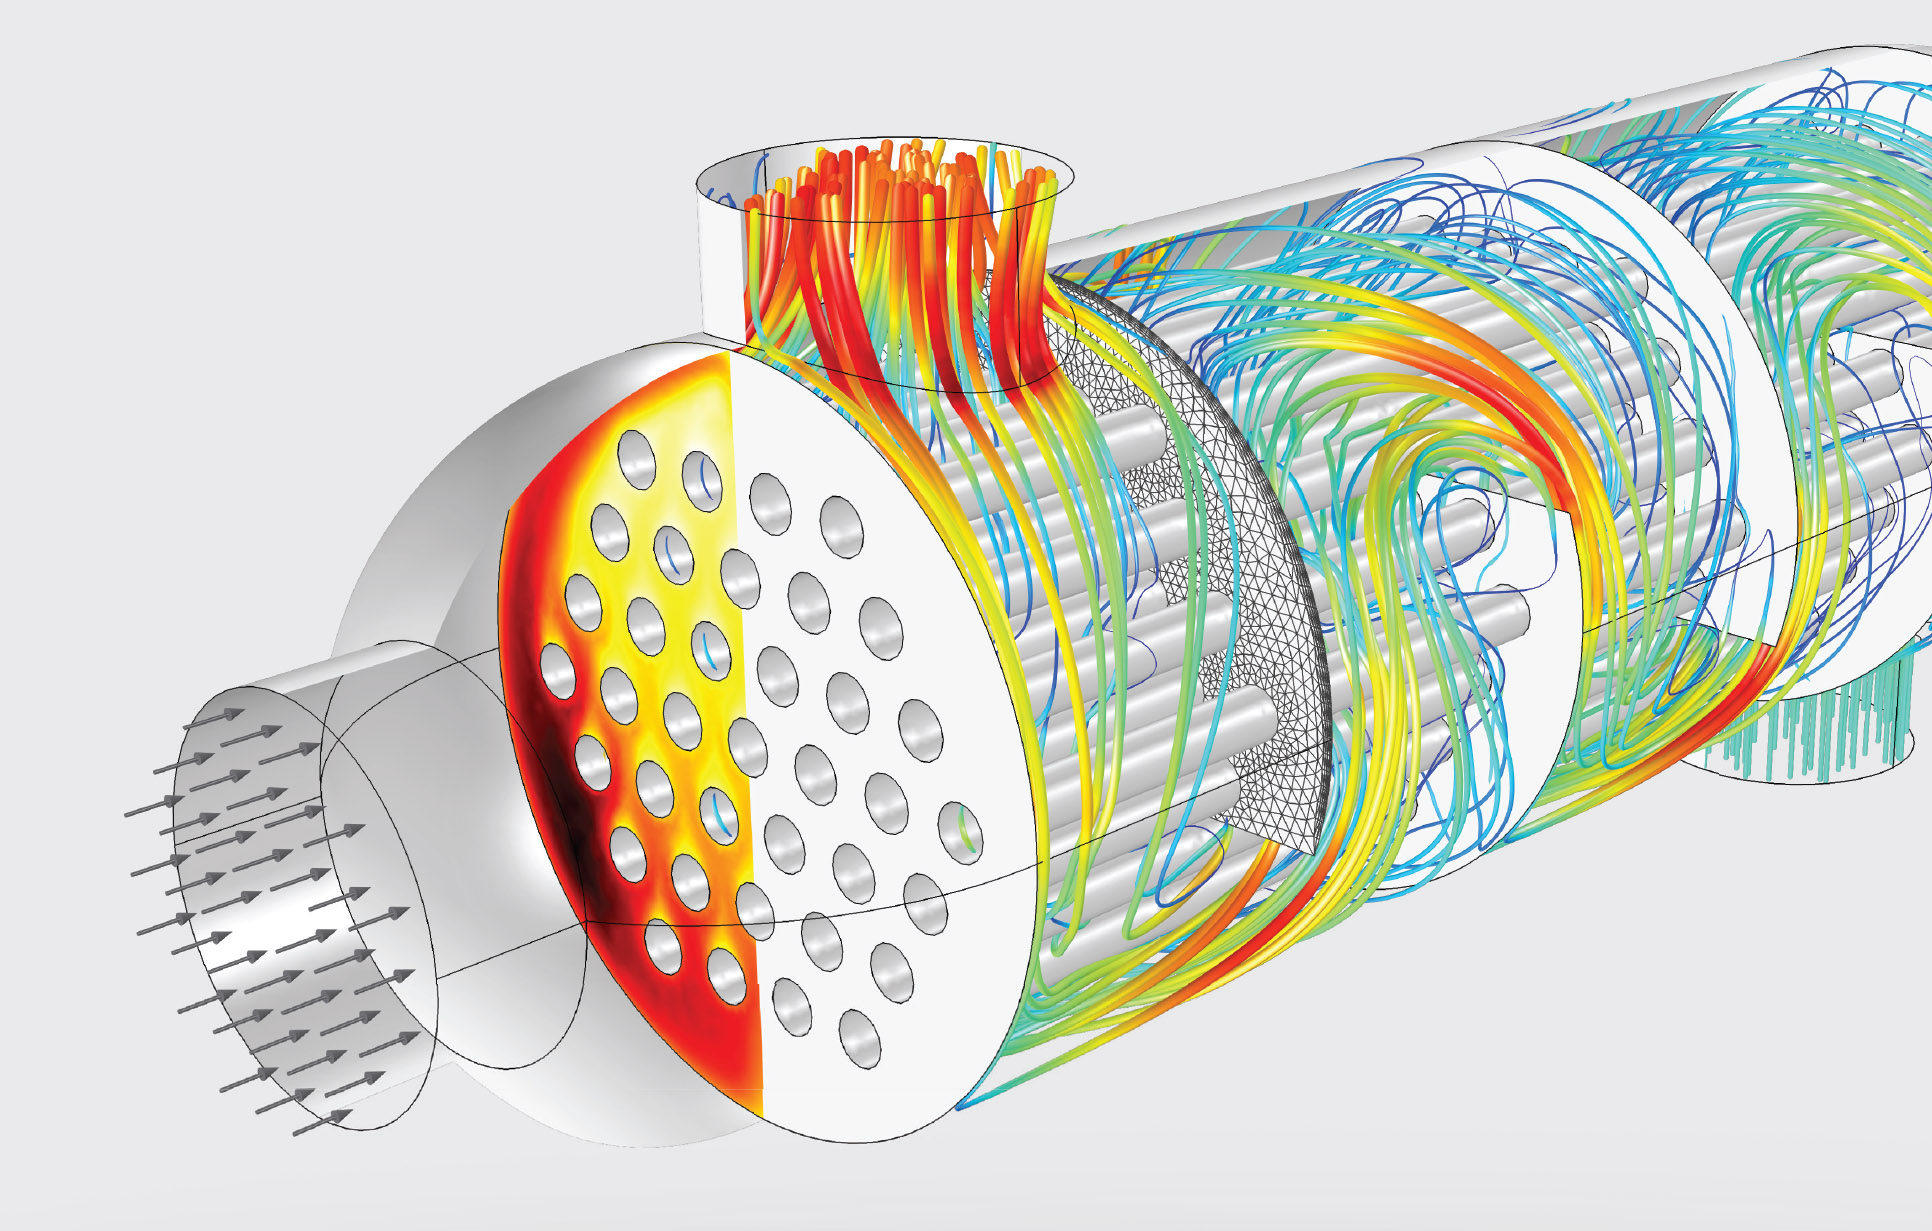
\includegraphics[width=0.8\textwidth]{figures/comsol-post-hoc-viz.jpg}
	\caption{Example of post-hoc visualization with applied post-processing techniques.}
	\label{fig:comsol-post-hoc-viz}
\end{figure}

A Visualization Toolkit (VTK) exists as an open-source alternative to proprietary visualization software. It's fully programmable and it can be deployed on highly parallelized architectures with large core counts. It implements polygonal, glyphing and volume rendering for 3D data and plotting capabilities for creating 2D charts. API is provided for C++ with Python and Java wrappers \citep{hanwellVisualizationToolkitVTK2015}.

VTK has been implemented and integrated into large number of applications for scientific data visualizations, like ParaView, VisIt, 3D Slicer, Medical Imaging Interaction Toolkit and so on. The aforementioned ParaView is worth a more detailed mention. It is developed by the team behind VTK (Kitware, Inc.) and integrates all the programmable parts of it into the cohesive experience packaged as desktop client application with GUI. Besides all of the classic tools for preparing the quality visualization output, it can render 3D content into virtual reality headsets like Oculus Rift or HTC Vive \citep{paraview2005}. Both VTK and ParaView can leverage parallel architectures with built-in Message-Passing Interface (MPI) support.


% prepisat, z abstraktu od Keplera
%Scientific visualization for exascale computing is very likely to require in situ processing. Traditional simulation checkpointing and post hoc visualization will likely be unsustainable on future systems at current trends due to the growing gap between I/O bandwidth and FLOPS. As a result, the majority of simulation data may be lost if in situ visualization techniques are not deployed. In situ visualization in this paradigm will be given unprecedented access to simulation output, potentially being able to process all relevant simulation output at every simulation time step, allowing for very high temporal fidelity compared to traditional post hoc visualization. However, this access poses many challenges in terms of data management, resource management and sharing, algorithm development and design, and implementation approaches. Currently, the community primarily relies on two in situ techniques: tightly coupled (on the same resource as the simulation) and loosely coupled (not sharing resources with the simulation). Each of these approaches have positive and negative factors which affect their performance under different simulation, resource, and visualization type constraints. Meaning, that for every given visualization task, it is not generally known which method would give the best performance on every data type, architecture, and set of resource constraints. Due to the lack of research and development on this topic it is still an open research problem requiring future research
%\citep{kressSituVisualizationTechniques}



\subsection{Real-time Visualization}
\label{rt-viz}
% DONE
Real-time simulation, i.e. the ability to simulate a virtual system as fast as the real system would evolve, can be beneficial to many engineering applications. To achieve real-time fluid flow simulation, numerical methods need to be selected carefully to make full use of the hardware capabilities. Generally, these were often simplified for use in games with lower accuracy, as the focus in gaming environments is more on creating visually appealing animation rather than aiming for physical accuracy \citep{delboscRealTimeSimulationIndoor}.

The Lattice-Boltzmann method in context of CFD simulations is ideally suited to acceleration on GPUs due to its spatial and temporal locality. Thanks to this they have extremely high computational throughput compared with traditional CFD methods. Therefore, with such method as LBM, it is now possible to achieve sound physical accuracy and good enough speed to reach real-time simulation capabilities.

The progress of scientific computations can be viewed in real-time thanks to the high-performance OpenGL visualization library called Forge. It is developed by the same team behind ArrayFire and distributed together with their library for high-performance parallel computing. The main challenge of optimizing the GPU code is reducing the amount of copying between CPU and GPU. It is written specifically for use with GPU-accelerated applications as it doesn't require the expensive copying from GPU to CPU and back to GPU for rendering, but instead it builds on CUDA/OpenCL interoperability with OpenGL and allows for direct reading of the data on GPU \citep{forge2016}. Forge provides various plotting and visualization functions for 2D and 3D domains.

\begin{figure}[!ht]
	\centering
	\subfloat[Common visualization pipeline.\label{fig:viz-classic}]{%
		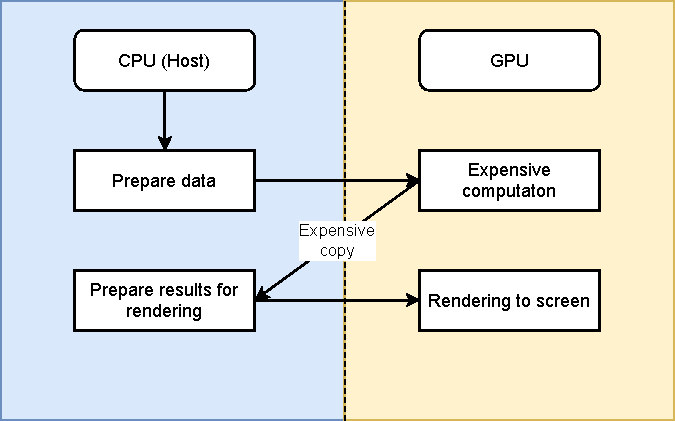
\includegraphics[width=0.51\textwidth]{figures/viz-classic.pdf}%
	} \qquad
	\subfloat[High-performance visualization pipeline.\label{fig:viz-forge}]{%
		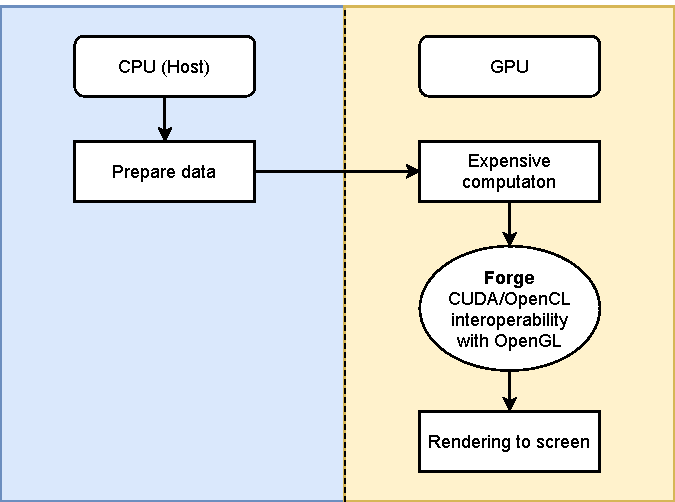
\includegraphics[width=0.43\textwidth]{figures/viz-forge.pdf}%
	}
	\caption{Differences between CPU-bound visualization with expensive copying bottleneck and high-performance GPU-bound visualization keeping full speeds of high-bandwidth of PCIe interface.}
	\label{fig:viz-forge-main}
\end{figure}

Practical scientific simulations for in-depth study of complex physical phenomena from real world, e.g. direct numerical simulation of cellular blood flow \citep{kotsalosDigitalBloodMassively2019}, requires higher accuracy. Instead of single-precision floating-point type (\texttt{f32}) computation, double-precision floating-point (\texttt{f64} has to be chosen. In LBM context, this practically doubles the amount of memory needed. For real-time visualizations of results with this type of precision, they have to be converted to a single-precision floating-point for Forge to effectively work with the data. In ArrayFire (and generally in programming), function for this operation is called \texttt{cast} (Alg. \ref{forge-cast-f32}).

\begin{lstlisting}[language=Rust, caption={Converting to single precision floating point for Forge visualization in C, C++ and Rust}, label=forge-cast-f32]
	// C
	af_array A_f64 = af_randu(100,100);
	af_array B_f32;
	cast(*B_f32, A_f64, f32);
	// C++
	array A_f64 = randu(100,100);
	array B_f32 = A_f64.as(f32);
	// Rust
	let dims = af::Dim4::new(&[100, 100,  1, 1]);
	let A_f64 = af::randu::<f64>(dims);
	let B_f32 = A_f64.cast::<f32>();
\end{lstlisting}

While developing the C++ and Rust implementations of LBM simulation backend, we used \texttt{image()} and \texttt{vector_field_2()} functions from Forge library for visualizing density and velocity of both lid-driven cavity and Kármán vortex street test cases in 2D (Figure~ \ref{fig:d2q9_lid} and Figure~ \ref{fig:d2q9_channel}).

\begin{figure}[!ht]
	\centering
	\subfloat[Visualization of lid-driven cavity simulation.\label{fig:d2q9_lid_5000_viz}]{%
		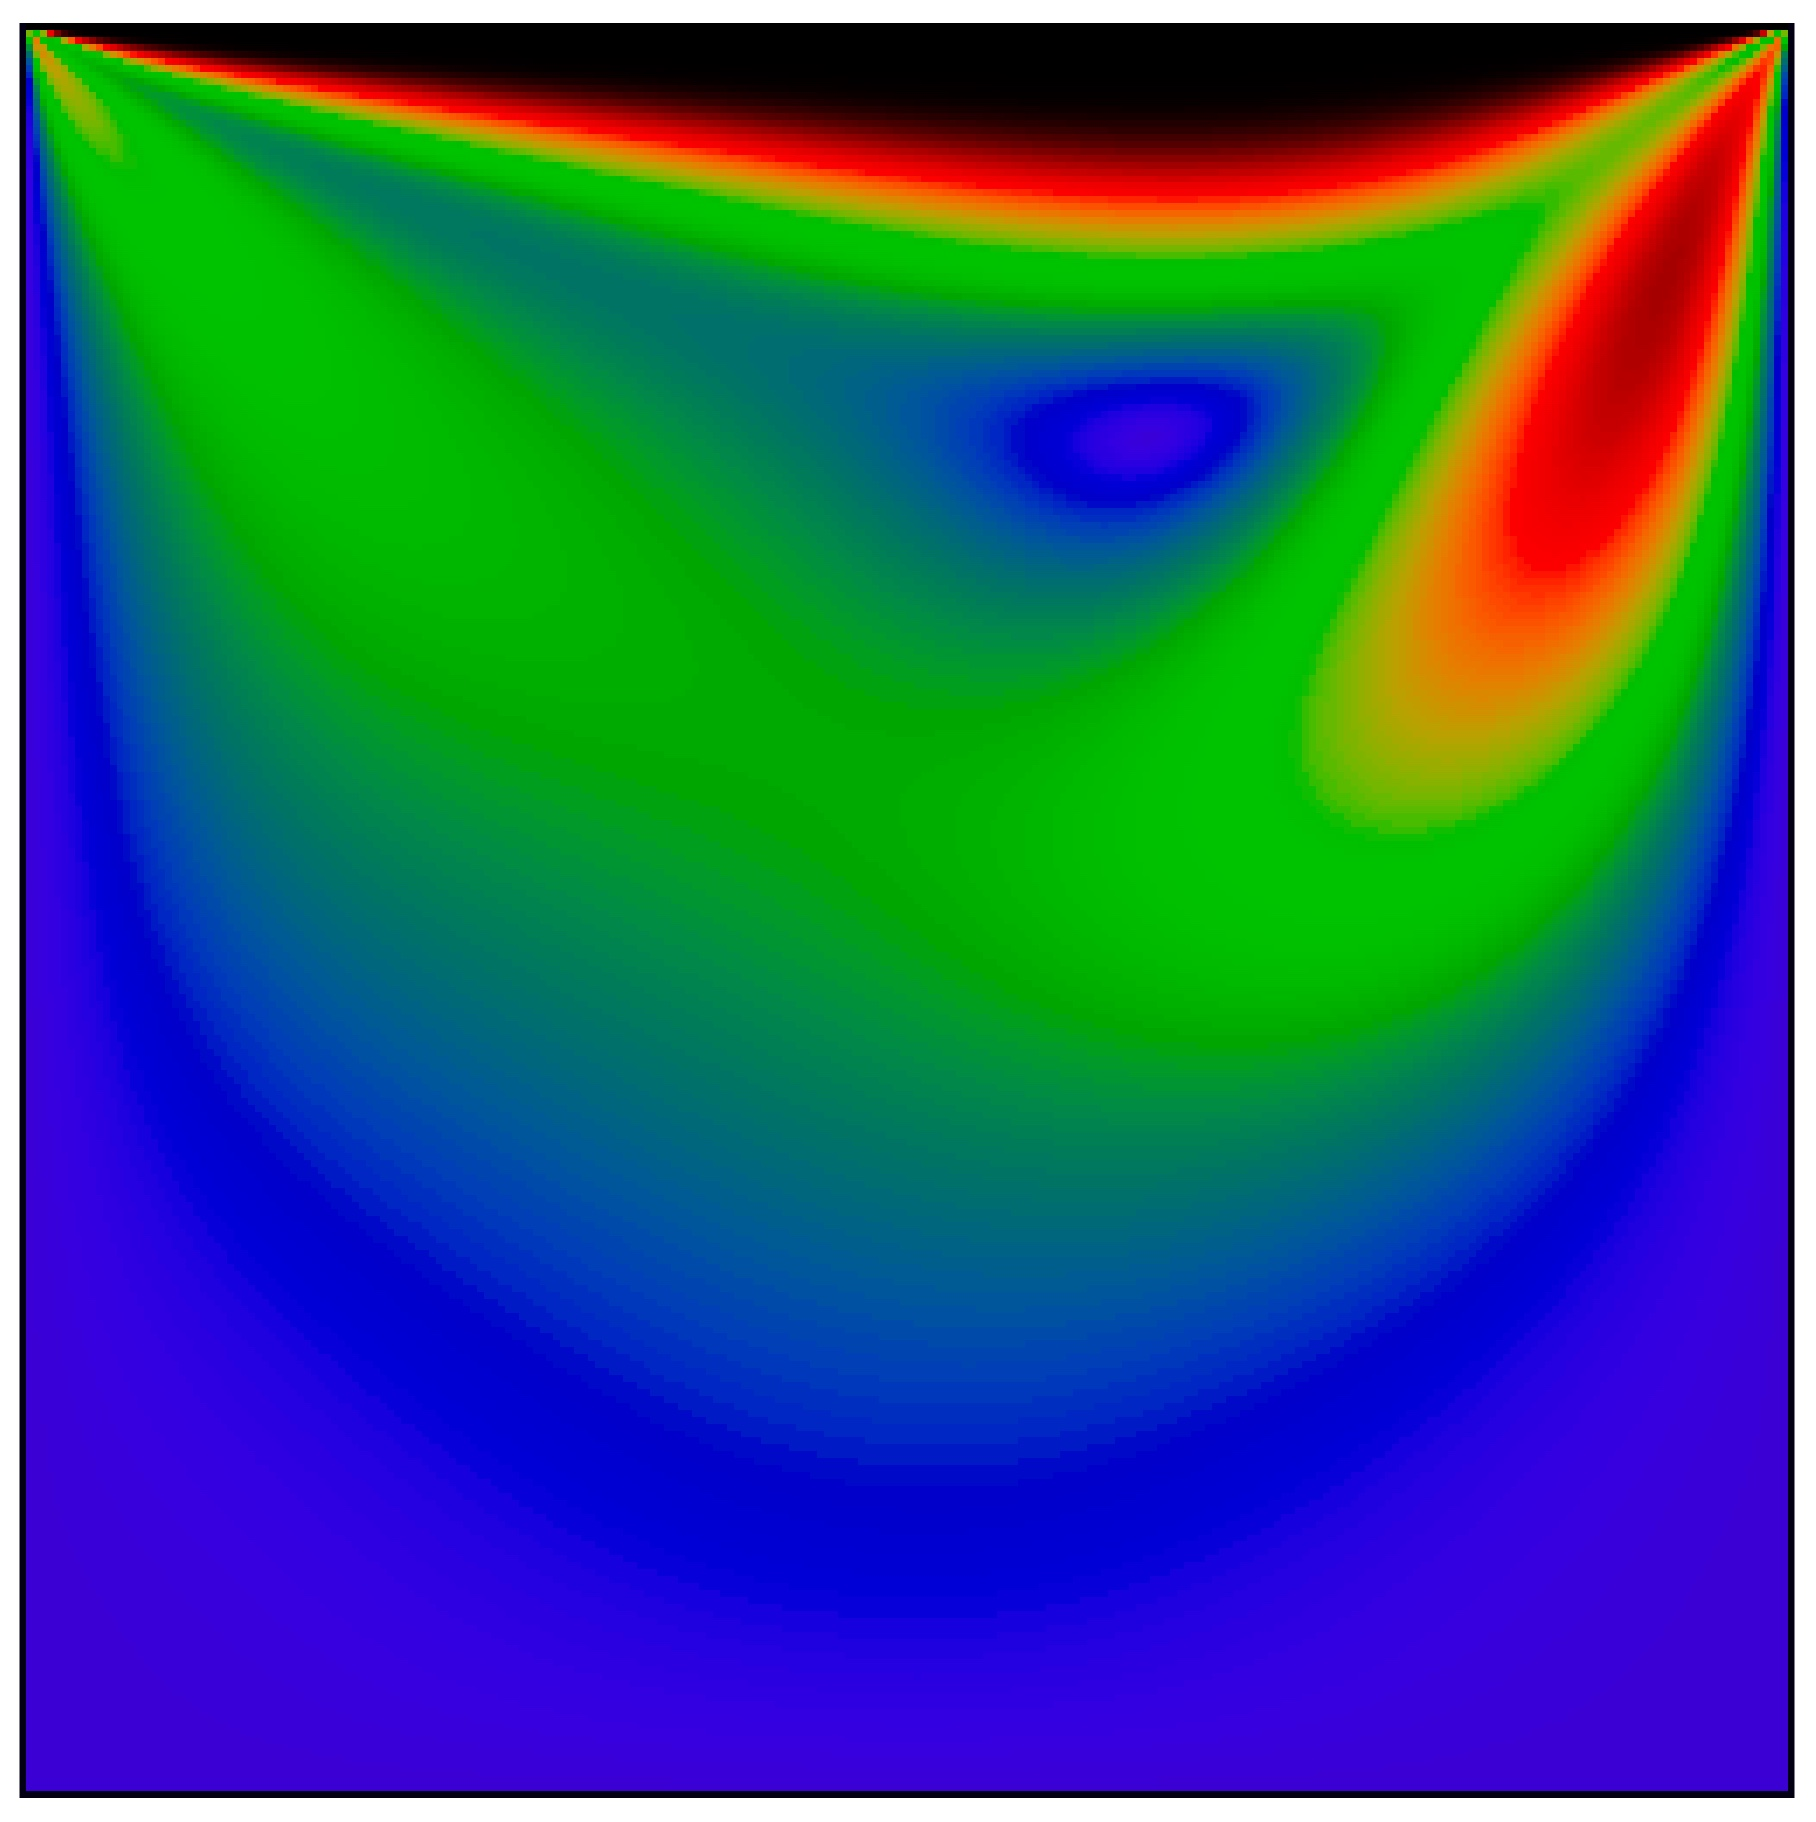
\includegraphics[width=0.3\textwidth]{figures/d2q9_lid_5000_viz.jpg}%
	}\qquad
	\subfloat[Velocity vector field.\label{fig:d2q9_lid_5000_u_field}]{%
		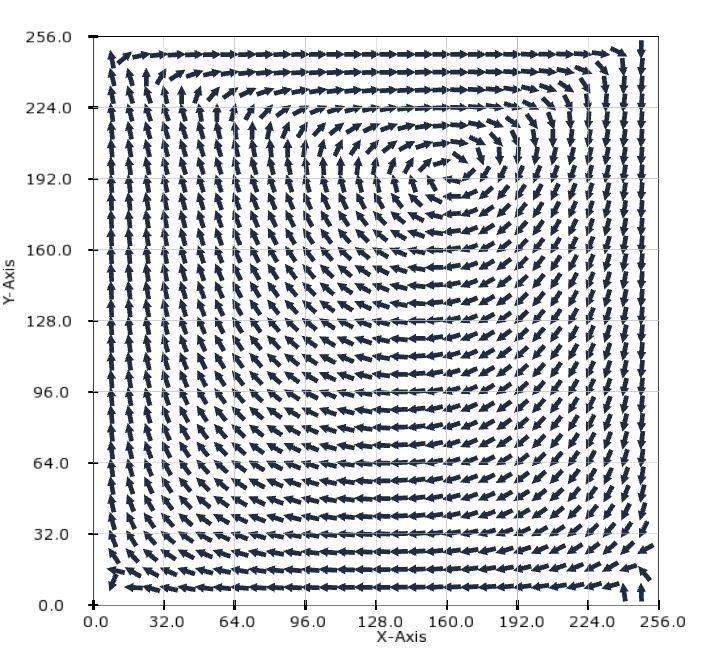
\includegraphics[width=0.335\textwidth]{figures/d2q9_lid_5000_u_field.jpg}%
	}
	\captionsetup{justification=centering}
	\caption{Lid-driven cavity test case at 128$\times$128 resolution after 5000 iterations.}
	\label{fig:d2q9_lid}
\end{figure}

\begin{figure}[!ht]
	\centering
	\subfloat[Visualization of Kármán vortex street simulation.\label{fig:d2q9_channel_5000_viz}]{%
		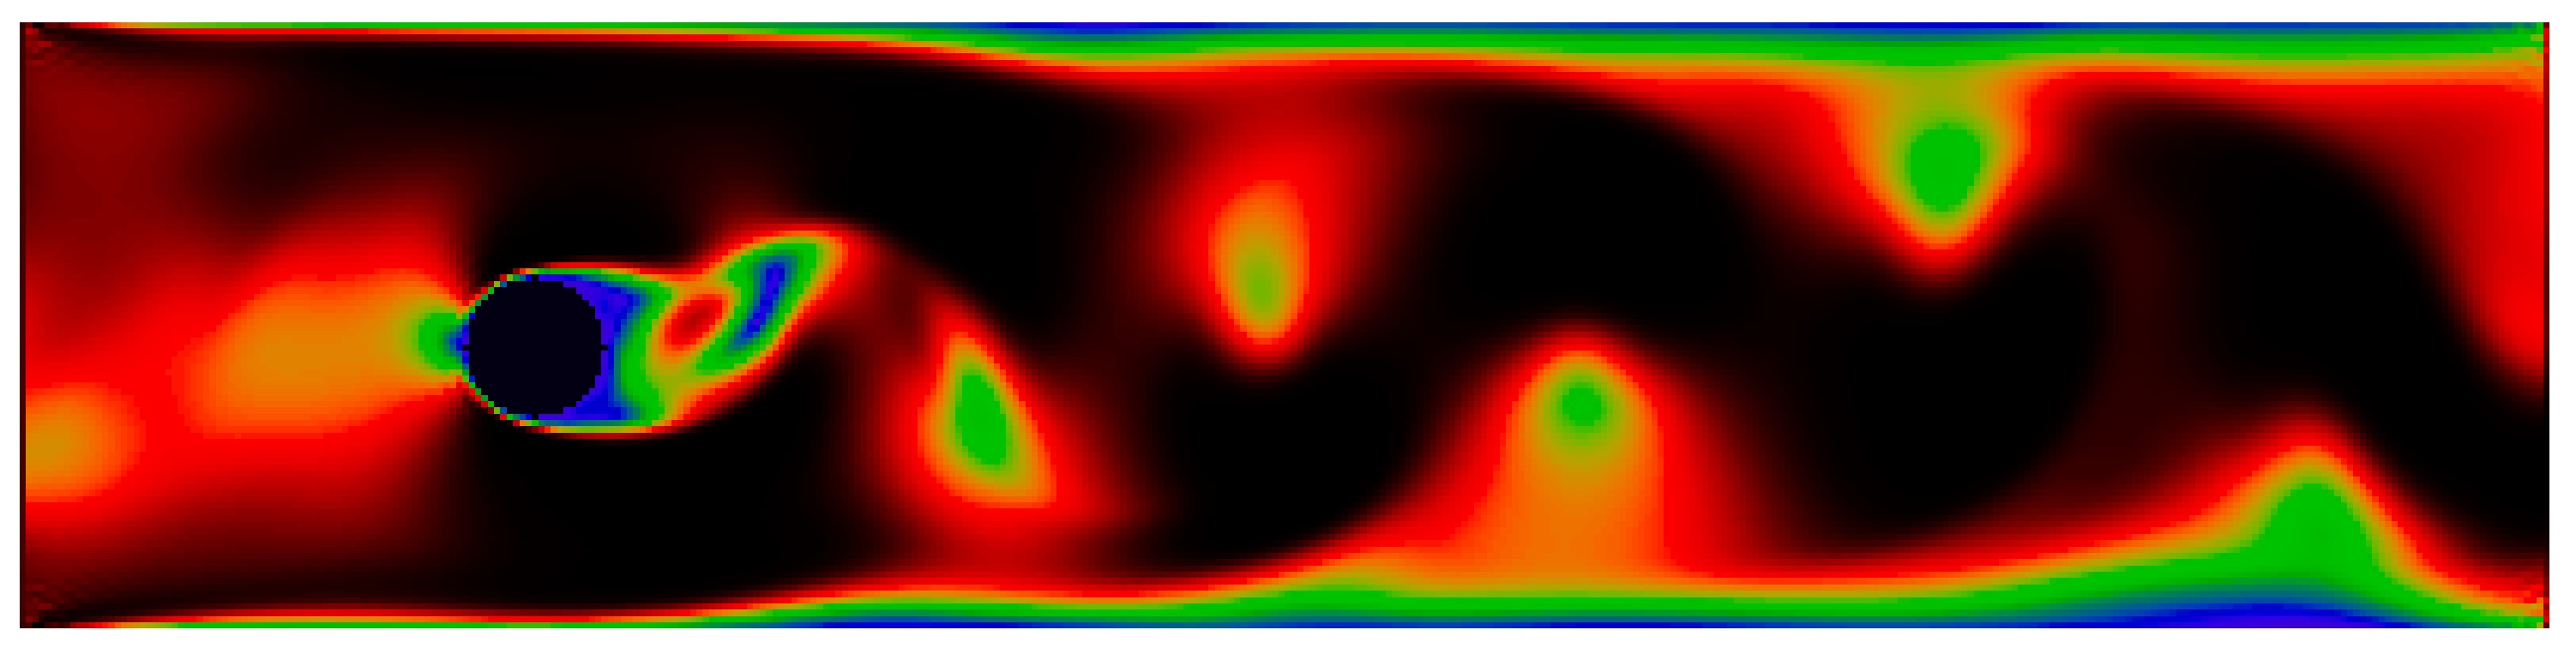
\includegraphics[width=0.63\textwidth]{figures/d2q9_channel_5000_viz.jpg}%
	} \par
	\subfloat[Velocity vector field (filtered for better presentation).\label{fig:d2q9_channel_5000_u_field}]{%
		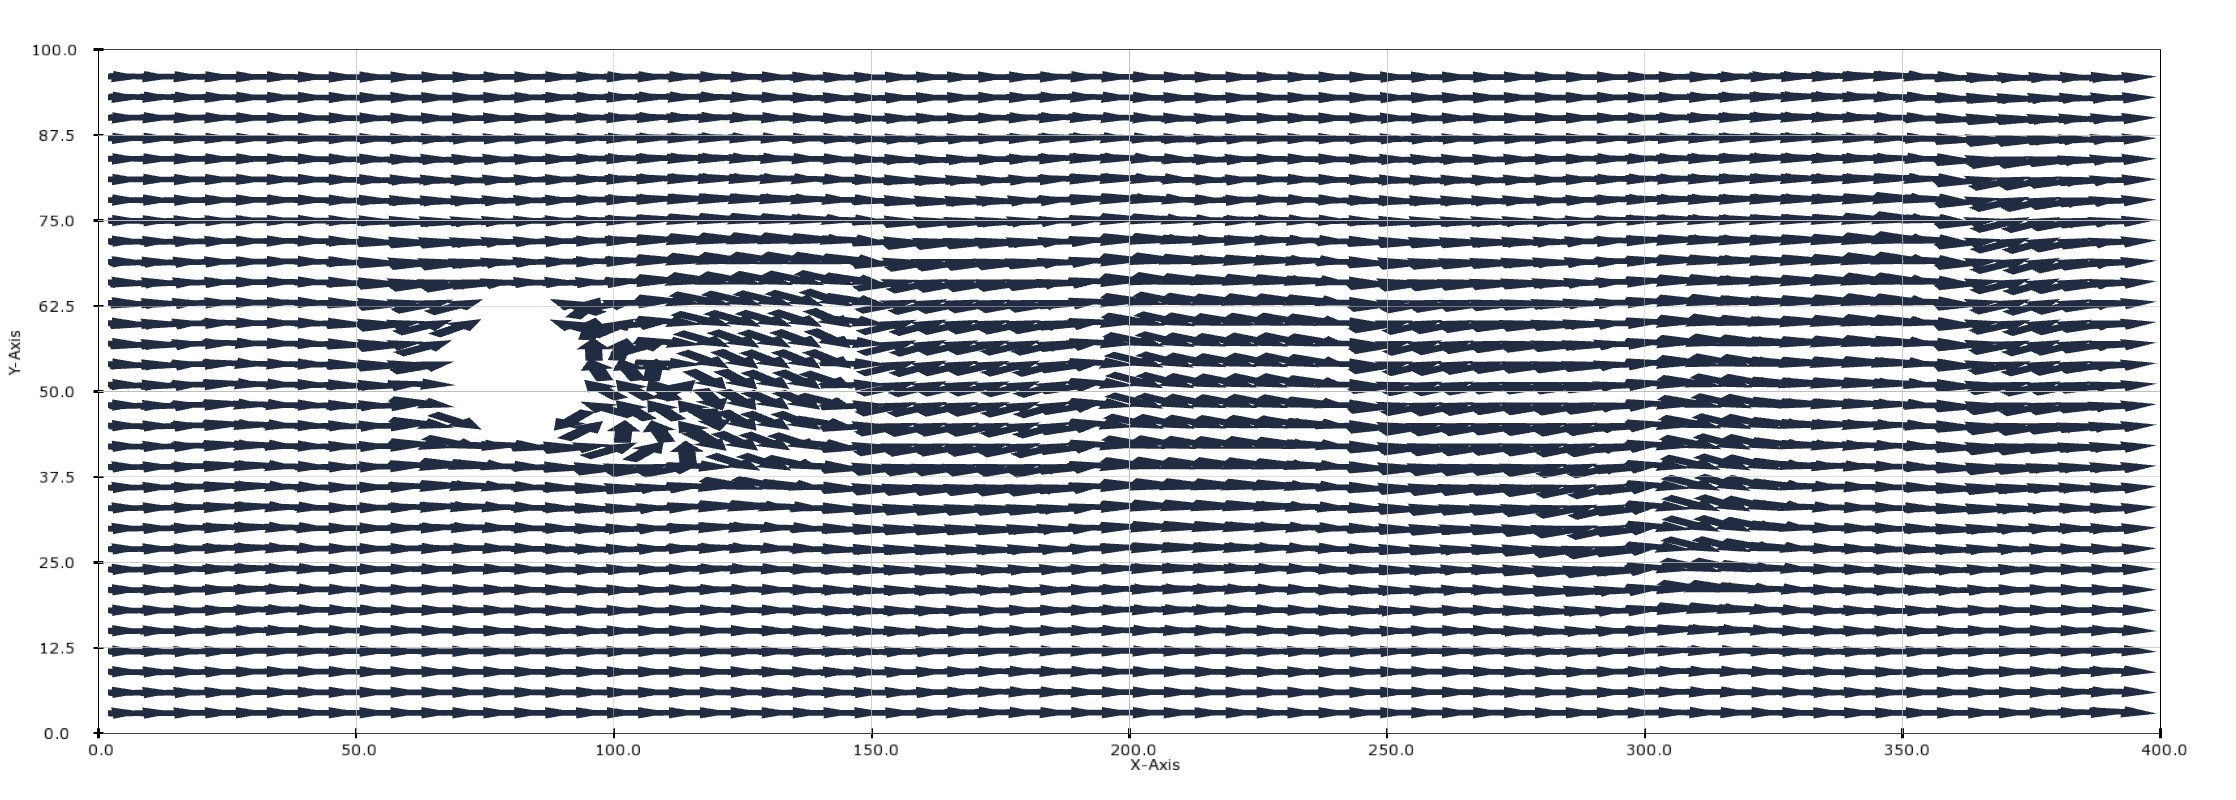
\includegraphics[width=0.65\textwidth]{figures/d2q9_channel_5000_u_field.jpg}%
	}
	\caption{Kármán vortex street (channel flow past circle-shaped obstacle) test case at 1000$\times$300 resolution after 5000 iterations.}
	\label{fig:d2q9_channel}
\end{figure}

% Visualizations can be zoomed, panned and rotated with a mouse.

\subsection{Interactive Visualization}
\label{interactive-simulation}
% DONE
Interpreting simulation results is often a laborious process. Already few decades ago, it was clear that to understand fluid phenomena in depth, we should move towards interactive simulation \citep{frischLatticeGasAutomataNavierStokes1986}. This would allow run-time manipulation of geometrical and physical simulation variables, opening ways to rapidly and intuitively investigate different scenarios and design configurations.

Recently, the increase of computational power and advances in general-purpose computing on GPUs (GPGPU) made this possible  \citep{delboscRealTimeSimulationIndoor, harwoodParallelisationInteractiveLatticeBoltzmann2017, kolihaOnlineVisualizationInteractive2015, glessmerUsingInteractiveLattice2017}. Together with the performance and speed of the LBM method, it's now possible to compute several hundreds of iterations per second which makes an interaction with the simulation in progress possible \citep{wangInteractive3DFluid2019}. Getting instant feedback according to the change of various parameters in simulation gives researchers the ability to iterate faster toward the creation of accurate model, better understanding of underlying phenomena, or employing simulation within the control of industrial systems. It is therefore desirable to push the limits of execution speed of LBM simulations.

Main goal to implement LBM algorithms for our simulation software is the ability to perform high performance computation and still keep the CPU free to do the additional work. The reason for it is that the visualization part is performed in virtual reality, which needs most of the CPU resources for processing the user tracking. Thanks to the fact that ArrayFire library was used, many hardware-specific optimizations were done for us behind-the-scenes. Although, there is growing body of work on optimizing LBM simulations \citep{wangInteractive3DFluid2019, wittmannLatticeBoltzmannBenchmark2018, tranPerformanceOptimization3D2017, kornerParallelLatticeBoltzmann2006, harwoodParallelisationInteractiveLatticeBoltzmann2017, harwoodREALTIMEMODELLINGSIMULATION}. We used some of the methods described in these articles. They are described in section \ref{optimizations-for-gpu}.

\subsubsection{Steering the Running Simulation}

When the simulation together with visualization are fast enough to stream live data to the screen, it's convenient to send signals to the simulation to change itself with updated parameters. This way, the model optimization can be sped up as the finding if result of the simulation is incorrect can happen much faster. Detecting a simulation that will  \citep{kreylos2002}


%Because of the difficulty of editing simulations by hand, computer graphics researchers have also considered how to control physics-based simulations. However, instead of the inefficient forward gradient computation, we use a technique, the adjoint method, that is orders of magnitude more efficient. This allows us to fully control 3D simulations in a fraction of the time
%\citep{mcnamaraFluidControl2004}

% upravit a povyberat co treba
Designing the behavior of an interactive object requires understanding and handling a large number of variables linked to: the function of the object (what-level), the way the function is accomplished (how-level) and the way a user experiences that function (why-level). Traditionally HCI uses a paradigm based on ``efficiency" to drive the design process, but recently integrated an aesthetics approach as a way to design the behavior from an experiential, rather than a functional, point of view ...  \citep{spadaforaDesigningBehaviorInteractive2016}

When dealing with interactive objects, we deal with Pragmatist Aesthetics. This kind of aesthetics underlines “how people experience the world dialogically as embodied subjects”

\citep{spadaforaDesigningBehaviorInteractive2016}.

\subsubsection{Time Manipulation}

To really understand the nature of the processes, we have to build a better tools for "seeing" and experimentation on demand. 

The computer is a medium of dynamic pictures -- visualizations driven by parameters and data.
\citep{victorInventingOnPrinciple2018}

\begin{figure}[!ht]
	\centering
	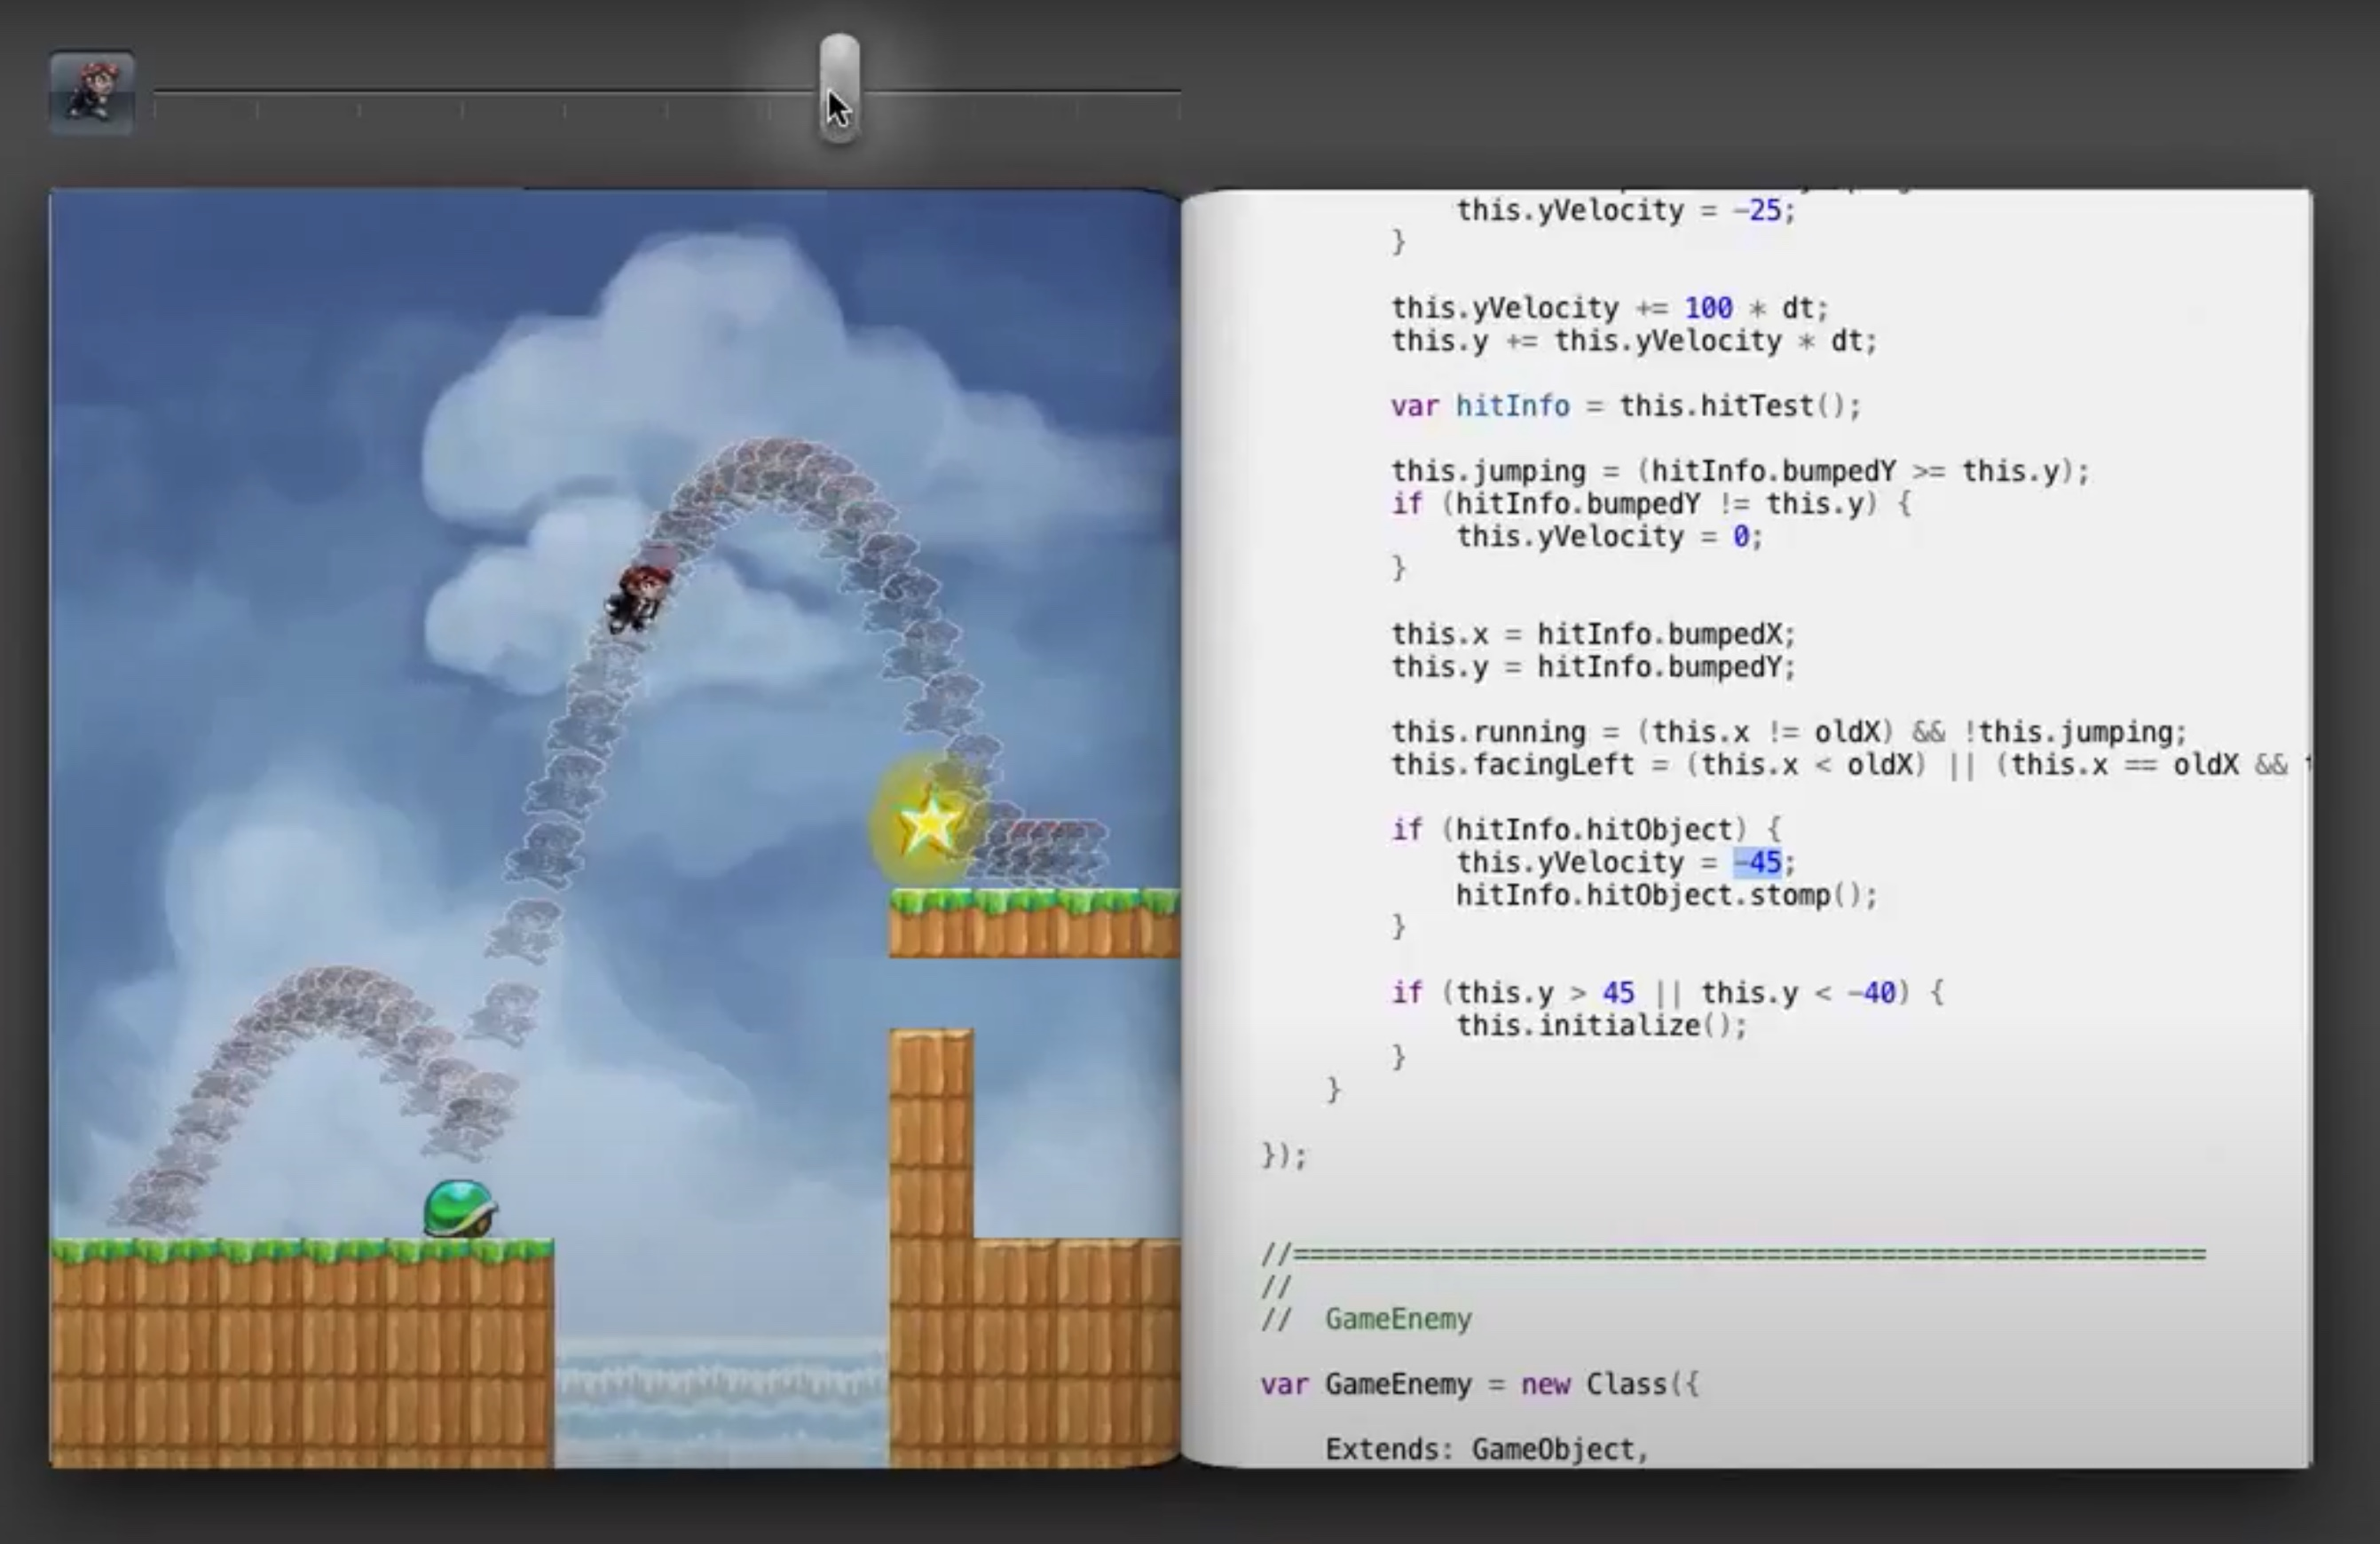
\includegraphics[width=0.9\textwidth]{figures/victor-time-manip.jpg}
	\caption{ \citep{victorInventingOnPrinciple2018}.}
	\label{fig:victor-time-manip}
\end{figure}

\subsection{Virtual and Augmented Reality}\label{sec:vrar}

Non-immersive interactive visualization systems implemented for the conventional desktop and mouse are effective for moderately complex problems. Immersive virtual environments, by comparison, lie at the other end of the spectrum and permit looking around an object by moving user's head position.

Therefore, a fundamental difference between desktop-and-mouse virtual realia and immersive VR is that the latter is a true 3D representation that may be either viewer or object-centered while the first is exclusively viewer-centered. In other words, changes in the relative positions of a 2D object’s components result from shifts in the viewer’s perspective. The same may be true for objects viewed in a three dimensional environment, whether real or virtual. However, in such an environment, an object may also appear to change shape (e.g., through foreshortening), not due to an altered position of the viewer, but because the ob- ject itself has moved to a different position. Immersive virtual reality displays aid in the unambiguous display of these structures by providing a rich set of spatial and depth cues. Virtual reality interface concepts allow the rapid and intuitive exploration of the volume containing the data, enabling the phenomena at various places in the volume to be ex- plored, as well as provide simple control of the visualization environment through inter- faces integrated into the environment \citep{brysonVirtualRealityScientific}.

Desktop-and-mouse interfaces for 3D visualizations make it difficult to specify positions in three dimensions and do not provide unambiguous display of 3D structure. Virtual reality interfaces attempt to provide the most anthropomorphic interfaces possible - that means they must be human-conforming and should be designed to allow the most natural, unambiguous way of scientific exploration. They must include two components: display and user control. Scientific visualization makes particular demands on virtual reality displays. The phenomena to be displayed in a scientific visualization application often involve delicate and detailed structure, requiring high-quality, high-resolution full-color displays. A wide field of view is often desirable, because it allows the researcher to view how detailed structures are related to larger, more global phenomena.

Historically, the early attempts at using head-mounted virtual reality technologies started with CRT-based Binocular Omni-Oriented Monitor (BOOM) created by Fakespace Systems Inc. BOOM was a stereoscopic display device with screens and optical system housed in a box that is attached to a multi-link arm. Head tracking was accomplished via sensors in the links of the arm that holds the box.

Advent of commodity-level VR hardware like HTC Vive or Oculus Touch has made this technology accessible for meaningful applications. These headset utilize lasers and photosensitive sensors (HTC Vive) or cameras (Oculus Touch) for head and hands tracking and provide six degrees of freedom (6DoF) for movement in virtual environment. By immersing the user into the simulation itself, virtual reality reveals the spatially complex structures in computational science in a way that makes them easy to understand and study. But beyond adding a 3D interface, virtual reality also means greater computational complexity \citep{brysonVirtualRealityScientific}. The ability to provide real-time interaction can provide strong depth cues, either through allowing interactive rotations or through the use of head-tracked rendering. Applications and techniques are being developed to discern how immersive technology benefits visualization. The medical field provides an especially promising context for this development, as medical practitioners require a thorough understanding of specific 3D structures: human anatomy. Users may interact simultaneously with high resolution computed tomography (CT) scans and their corresponding, 3D anatomical structures.

With the addition of inside-out tracking in VR headsets like Widows Mixed Reality and Oculus Quest, it brought the hand tracking support into the software development kits for each platform. More and more VR developers started to leverage the hand tracking in the interfaces of their applications. Thanks to the growth of gestures usage in virtual reality and embodied cognition, there have been various new technologies developed to either improve the modelling efficiency, or to provide more nature intuitive experience to the users \citep{dangetiComparingBarehandinairGesture2016}.

Another frequently used type of immersive, interactive display technology nowadays is projection-screen-based Cave Automatic Virtual Environment (CAVE). These systems consists of 3 to 6 large displays positioned into a room-sized cube around the observer. The walls of a CAVE are typically made up of rear-projection screens, but recently the flat panel displays are commonly used. The floor can be a downward-projection screen, a bottom projected screen or a flat panel display. The projection systems are very high-resolution due to the near distance viewing which requires very small pixel sizes to retain the illusion of reality. The user wears 3D glasses inside the CAVE to see 3D graphics generated by the CAVE. People using the CAVE can see objects apparently floating in the air, and can walk around them, getting a proper view of what they would look like in reality. This is made possible by infrared cameras. Movement of the observer in the CAVE is tracked by the sensors typically attached to the 3D glasses and the video continually adjusts to retain the viewers perspective.

Many universities and engineering companies own and use CAVE systems. Researchers can use these systems to conduct their research topic in a more effective and accessible method. Engineers have found them useful in enhancing of a product development through prototyping and testing phases.

Substantial amount of work in applying 3D visualizations and virtual reality for solving technological issues and bringing new trends into steelmaking industry is currently happening at Center for Innovation through Visualization and Simulation (CIVS) at Purdue University Northwest (located in Indiana, USA). CIVS has been globally recognized for its integrated and application-driven approaches through state-of-the-art simulation and virtual reality visualization technologies for providing innovative solutions to solve various university research problems, industry issues, as well as education. More than 350 projects that have been completed at the center from its inception in 2014 until today provided substantial educational and economic impact, resulting in more than 40 million US dollars in savings for companies.

One can say that virtual reality established itself in many disciplines of human activities, as a medium that allows easier perception of data or natural phenomena appearance.

% ----------------------------------------------------------------

%\section{Human-Computer Interface}
%
%% upravit a povyberat co treba
%Designing the behavior of an interactive object requires understanding and handling a large number of variables linked to: the function of the object (what-level), the way the function is accomplished (how-level) and the way a user experiences that function (why-level). Traditionally HCI uses a paradigm based on ``efficiency" to drive the design process, but recently integrated an aesthetics approach as a way to design the behavior from an experiential, rather than a functional, point of view ...  \citep{spadaforaDesigningBehaviorInteractive2016}
%
%When dealing with interactive objects, we deal with Pragmatist Aesthetics. This kind of aesthetics underlines “how people experience the world dialogically as embodied subjects”
%
%\citep{spadaforaDesigningBehaviorInteractive2016}.

%\subsubsection{SCADA}
%
%% upravit https://www.dpstele.com/scada/how-systems-work.php
%Supervisory Control and Data Acquisition (SCADA) is a system that aims to monitor and control field devices at your remote sites. SCADA systems are critical as it helps maintain efficiency by collecting and processing real-time data.
%
%SCADA is a centralized system that monitors and controls the entire area. This supervisory system gathers data on the process and sends the commands control to the process.
%
%The main goal of this supervisory system is to monitor and control equipment in the industrial processes for companies in the public and private sectors. As a matter of fact, in today's world, there are SCADA systems almost everywhere. This includes industrial plants, manufacturing, transportation, oil and gas, power distribution, water control and etc.
%
%Four SCADA Functions:
%
%\begin{enumerate}
%	\item Data acquisition
%	\item Networked Data Communication
%	\item Data presentation
%	\item Control
%\end{enumerate}
%
%In data acquisition, the collection of SCADA data frequently involves some kind of analog to digital conversion. Temperature is converted to degrees Celsius. Transmit signal strength is converted to dBm. Channel quality is measured in errored seconds. 
%
%The collected data is transmitted either spontaneously or in response to a request for data to some kind of upstream consolidator or master. The communication channel can be analog (T202, POTS) or digital (RS485, TCP/IP). SCADA network topology typically also includes some kind of transport validation independent of any content validation.
%
%
%The collected data is processed, organized and presented for system operators to make appropriate response and control decisions. The presentation can vary from tabular presentation of logged events to graphical presentation against mapping or image backgrounds.
%
%If control decisions are warranted and the system supports output, appropriate commands can be dispatched to affect specific operational or configuration changes. Most control actions are performed by RTUs and PLCs.
%
%Four main components of SCADA: inputs, remote telemetry units (RTUs),human-machine interface (HMI) and communication network.
%
%% Vysvetlenie preco SCADA nie je dostacujuca pre to co potrebujeme v real-time modsim a preco chceme VR
%
%SCADA systems provide an invaluable interface for working with real-time data from various processes. Especially for many in the business of data and natural sciences, SCADA is a rich source of real-world data on demand. It's been successfully coupled with the machine learning to work with high-frequency of large amounts of data \citep{linWindPowerPrediction2020}. 
%
%% trosku doplnit/prepisat
%The problem with visual design approaches in SCADA applications is that the interfaces was mostly limited to simple graphics like plots, simple 2D animations, animated gauges, interactive knobs etc. It can be argued that it's often not needed to have complex visuals in specialized SCADA applications and they are "good enough" for the job at hand.
%
%% nejake premostenie?
%
%An interesting look into the future of SCADA interfaces was presented in study by \cite{soeteMixedRealitySCADA2015}, in which they managed to implement a Augmented Reality (AR) supporting tool for SCADA application in simulated automated logistic process. It shows potential benefits of using VR and AR technologies in the development of supervisory control and support. AR and VR is fairly new and relatively unknown in the industry, so the integration of such technologies is still in its infancy.
%
%% Mozno spomenut este vyuztie computer vision libraries ako OpenCV (C++), ktore je potrebne vyuzit pre implementaciu mixed reality aplikacii v spojeni so SCADA systemami (sledovat co sa deje v realnom svete a dalej pracovat s tymito datami... spojit to s machine learningom a object recognition... 
%
%% doplnit/upravit aby to davalo zmysel.. mozno prehodit inde?
%To really understand the nature of the processes, we have to build a better tools for "seeing" and experimentation on demand. 

% ------------------------------------------------------

\section{Implementation of a Simulation Software} 

\subsection{Technology Stack} \label{sec:tech-stack}


The ArrayFire library is used for high-performance, cross-platform implementation of Lattice Boltzmann algorithm.

\subsubsection{Cross-platform Development with ArrayFire}

% prepisat (https://arrayfire.org/arrayfire-rust/book/vectorization.html)
%Programmers and Data Scientists want to take advantage of fast and parallel computational devices. Writing vectorized code is necessary to get the best performance out of the current generation parallel hardware and scientific computing software. However, writing vectorized code may not be immediately intuitive. ArrayFire provides many ways to vectorize a given code segment. In this chapter, we present several methods to vectorize code using ArrayFire and discuss the benefits and drawbacks associated with each method.

ArrayFire is a vectorized library. Most functions operate on Arrays as a whole i.e. on all elements in parallel.
%----

ArrayFire provides several different methods for manipulating arrays and matrices. The functionality includes:

\begin{itemize}
\item \texttt{moddims()} - change the dimensions of an array without changing the data
\item \texttt{flat()}  - flatten an array to one dimension
\item \texttt{flip()}  - flip an array along a dimension
\item \texttt{join()}  - join up to 4 arrays
\item \texttt{reorder()}  - changes the dimension order within the array
\item \texttt{shift()}  - shifts data along a dimension
\item \texttt{tile()}  - repeats an array along a dimension
\item \texttt{transpose()}  - performs a matrix transpose
\end{itemize}

The simulation part of the software solution presented in this thesis was built using ArrayFire, a cross-platform library for developing parallel algorithms. I picked it after considering other approaches like using bunch of different helper libraries together for vectorization and cross-compilation of C++ code for different GPU platforms. C++ is battle-tested language with plethora of available libraries and has been extensively used in CFD simulation software development. Although, I would have to optimize the code for specific GPUs and their distinctive features myself, writing extensive amount of code in the process. This is where the ArrayFire library shines the most: it provides hundreds of hand-tuned, low-level optimized functions for various domains including vector algorithms, image processing, computer vision, signal processing, linear algebra, statistics, and more. Writing complex algorithms that are automatically optimized for all kinds of hardware accelerators (GPUs, CPUs, FPGAs etc.) can be done in few lines of code instead of writing hundreds or thousands of lines of kernel code.

ArrayFire main API is written in C with additional wrappers for other languages like C++, Python, Rust and JavaScript. It provides hundreds of hand-tuned, low-level optimized functions for various domains including vector algorithms, image processing, computer vision, signal processing, linear algebra, statistics, and more.

It helped with simplifying the overall implementation and reducing lines of code (LoC).

To start developing cross-platform software with ArrayFire, first it has to be installed on a development machine. It can be installed by either using binary installer for Windows, Linux or OSX, or built from source.

The high-performance visualization library called Forge is bundled with the installer. It can be disabled in the installation process if user doesn't want to install it. I used it in throughout the development process to test early protypes, check if the output is visually correct and also benchmark the simulation software for what computational domain the visualization stays fast enough to show real-time output as the simulation is running.



\subsubsection{Rust as C/C++ Alternative} \label{sec:rust-alt}
% DONE
As an alternative to C++ programming language, I considered Rust. It has been chanted around the programming world as a language that could one day replace C or C++ as a go-to language for writing performant low-level applications and systems. The problem with going down the road of using Rust is that it's still considered a new language with developing ecosystem of libraries, often lacking the ones that are readily available in C/C++ ecosystem. Good thing is that it's growing daily. After reading through tens of articles about pros and cons of the language, I had to test it first and try developing some prototypes to find out for myself if it's worth developing such a complex application.

The main proposition of Rust language is that it helps you write faster, more reliable software. Traditionally, developers who were looking for the best raw performance as they can get to squeeze out of their programs by aggressively optimizing it, were mostly reaching out for C++ as it's possible to get down to low-level if needed. The object-oriented nature of C++ on the other hand allows for constructing code that is easier to reason about. But still, the high-level ergonomics and low-level control are often at odds in programming language design \citep{steveklabnik2018}. Developers are still responsible for managing the memory in C++ applications. This can lead to problems if application is not well architected or developers not being disciplined about memory cleanup after use.

Rust challenges the status quo of high-level ergonomics with low-level performance in one language. Its unique feature called ownership allows the compiler to make memory safety guarantees without the need of an garbage collector. When building low-latency software, garbage collection adds unwanted pauses to the execution time. 

The simulation backend (i.e. actual implementation of LBM solver) was written in both C++ and Rust programming languages to compare the resulting performance and overall development experience. Both of those versions perform very similarly, but since Rust is being very interesting to work with in term of memory-safety, it was picked as a winner. Therefore the simulation backend that is used in tandem with VR visualization frontend is actually implemented in Rust. 

\subsubsection{Hardware}
% DONE
The focus of this work was to build a high-performance simulation software with integrated VR visualization that can be used on variety of platforms. VR is readily supported on Windows systems, with bit of an additional tuning here-and-there on Linux distributions. MacOS is not supported from any platform as of today, but the hardware it runs on is not powerful enough anyway (this can change in not-so-distant future, though!). Hardware requirement for running the VR application that is described in this work is clearly displayed in Table~\ref{tab:vr-specs} in section \ref{sec:hardware-req} of Appendix A. The performance of simulation backend was thoroughly benchmarked. List of GPUs that was used throughout the development is clearly displayed in Table~\ref{tab:gpus} in section \ref{sec:hardware-gpus}.

% ---------------------------------------------------------

\subsection{Implementation of Lattice Boltzmann Method for GPUs}
% DONE
In this section, each step in the program lifecycle is presented, showing how different parts are constructed so they can be called from the Unity game engine (as a Native Plugin).

\subsubsection{Initialization}

In Rust, the common data structure for composing various types of data under one roof is \texttt{struct}. In our simulation implementation, \texttt{struct Sim \{...\}} stores the all parameters and other data structures that are needed during the program lifecycle. Structs can be instantiated in different ways. Most common way is via the constructor method \texttt{new()}. For proper constructing of \texttt{Sim} and its properties, the struct implementation has to be defined with \texttt{impl Sim \{...\}} (Listing~\ref{sim-struct}). Additional directive \texttt{\#[repr(C)]} is added on top of \texttt{Sim} struct to specify alternative data layout, specifically to represent it as how it would be done with C or C++ language. That means the order, size, and alignment of fields is exactly what would be expect from C or C++.

\begin{lstlisting}[language=Rust, caption=Implementation of Sim struct with constructor method., label=sim-struct]
#[repr(C)]
pub struct Sim {
	// ... all the fields are defined here
}

impl Sim {
	pub fn new(nx: u64, ny: u64, initial_density: f32, initial_ux: f32, omega: f32, obstacle_x: u64, obstacle_y: u64, obstacle_r: u64
	) -> Result<Sim, String> {
		// ... rest of the implementation
	}
}
\end{lstlisting}

The simulation program needs to be initialized at the start with correct parameters. These are passed into the \texttt{new()} constructor method as its arguments and then used for initialization in ArrayFire Arrays. There are number of independent Arrays being initialized in this method, such as discrete velocities, weights for computing particle distributions in equilibrium, etc. (Listing~\ref{independent-initial-params}).

\begin{lstlisting}[language=Rust, caption=Setting initial parameters that are independent from constructor method's input arguments., label=independent-initial-params]
let t1: f32 = 4. / 9.;
let t2: f32 = 1. / 9.;
let t3: f32 = 1. / 36.;
// Discrete velocities
let ex = Array::<f32>::new(&[0., 1., 0., -1., 0., 1., -1., -1., 1.], dim4!(9));
let ey = Array::<f32>::new(&[0., 0., 1., 0., -1., 1., 1., -1., -1.], dim4!(9));
// weights
let w = Array::new(&[t1, t2, t2, t2, t2, t3, t3, t3, t3], dim4!(9));
// Initial physical parameters
let mut density = constant::<f32>(initial_density, dim4!(nx, ny));
let mut ux = constant::<f32>(initial_ux, dim4!(nx, ny));
let mut uy = constant::<f32>(0.0, dim4!(nx, ny));
// ...
\end{lstlisting}

\subsubsection{Boundary Conditions}

Two types of boundary conditions, namely geometrical and physical, are implemented with ArrayFire Arrays as a mask on 2D or 3D grids. 

\begin{lstlisting}[language=Rust, caption=Setting the geometrical boundary conditions of circle in a pipe flow (2D Karmán vortex)., label=init-circle]
let mut bound = constant::<f32>(1.0, dim4!(nx, ny));
// circle
let r = constant::<f32>(obstacle_r as f32, dim4!(nx, ny));
let r_sq = &r * &r;
let circle = moddims(
	&le(
		&(pow(
			&(flat(&x) - obstacle_x as f32),
			&(2.0 as f32), false)
		+ pow(
			&(flat(&y) - obstacle_y as f32),
			&(2.0 as f32), false)
		),
		&flat(&r_sq),
		false
	),
	dim4!(nx, ny),
);
bound = selectr(&bound, &circle, 0.0 as f64);
// top
set_col(&mut bound, &constant::<f32>(1.0, dim4!(nx)), 0);
// bottom
set_col(
	&mut bound,
	&constant::<f32>(1.0, dim4!(nx)),
	ny as i64 - 1,
);
\end{lstlisting}


Physical and lattice parameters that are supplied to the simulation at the start so it can begin with something.

There is difference between initial conditions in BGK and MRT code.

- BGK \\

\begin{lstlisting}[language=Cpp, caption=C++ code for setting different computing backends., label=cpp-backends]
	#include <arrayfire.h>
	int main()
	{
		af::setBackend(AF_BACKEND_CUDA);
		// af::setBackend(AF_BACKEND_OPENCL);
		// af::setBackend(AF_BACKEND_CPU);
		return 0;
	}
\end{lstlisting}

- MRT \\

\begin{lstlisting}[language=Cpp, caption=C++ code for setting different computing backends., label=cpp-backends]
	#include <arrayfire.h>
	int main()
	{
		af::setBackend(AF_BACKEND_CUDA);
		// af::setBackend(AF_BACKEND_OPENCL);
		// af::setBackend(AF_BACKEND_CPU);
		return 0;
	}
\end{lstlisting}

\subsubsection{Streaming}

\begin{figure}[!ht]
	\centering
	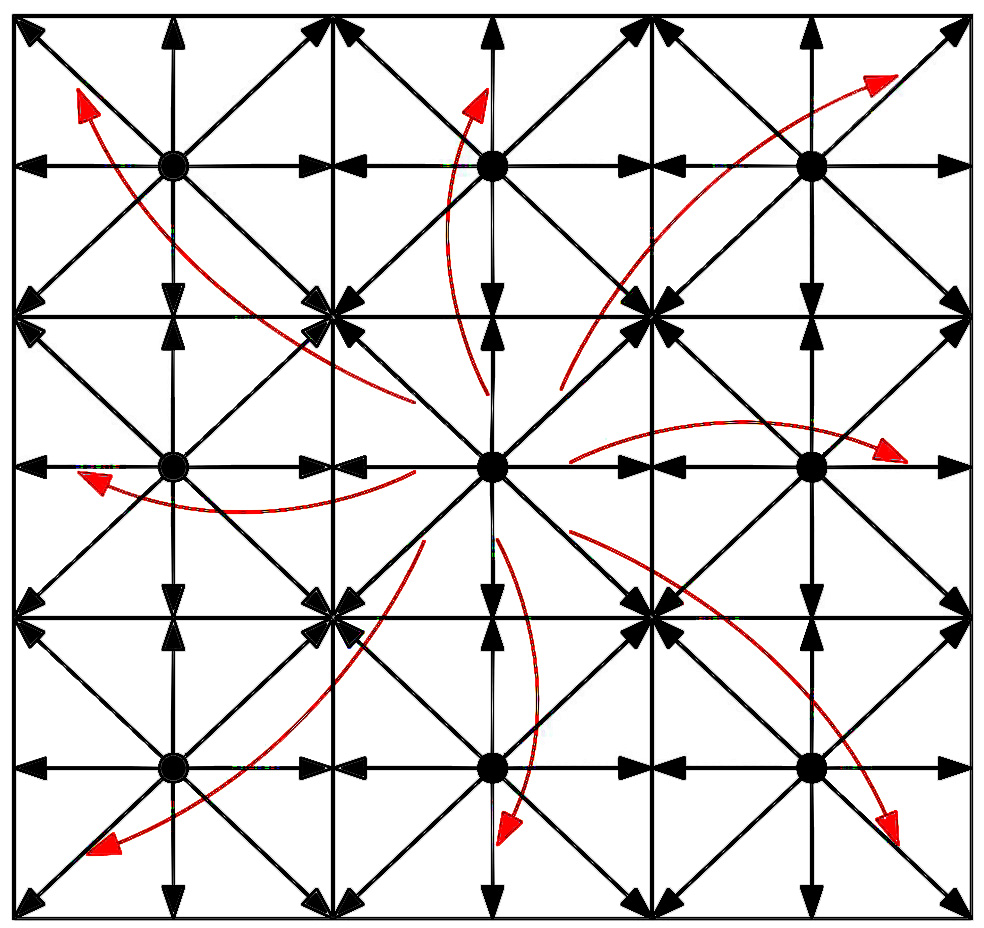
\includegraphics[width=0.7\textwidth]{figures/streaming.jpg}
	\caption{Illustration of the streaming step.}
	\label{fig:streaming}
\end{figure}

Streaming in general is usually treated as a separate step, implemented as a individual kernel, but also can be bundled together with the collision kernel to save memory, therefore boost speed.

In current implementation, the streaming is implemented as a shift of indices of neighbouring nodes. In this fashion, the index is pre-computed at the beginning and then used throughout the simulation lifetime to index into the particle distributions of neighbouring nodes.

\begin{lstlisting}[language=Rust, caption=Pre-computed streaming step in the way of shifting indices during the program intialization phase., label=rust-nb-index]
	let ci: Array<u64> = (range::<u64>(dim4!(1, 8), 1) + 1) * total_nodes;
	// Indices ordered to reflect a direction to the neighbouring nodes
	let nbidx = Array::new(&[2, 3, 0, 1, 6, 7, 4, 5], dim4!(8));
	let span = seq!();
	let nbi: Array<u64> = view!(ci[span, nbidx]);
	
	let main_index = moddims(&range(dim4!(total_nodes * 9), 0), dim4!(nx, ny, 9));
	let nb_index = flat(&stream(&main_index));
\end{lstlisting}

2D \\

\begin{lstlisting}[language=Rust, caption=Streaming with \texttt{shift} function for two dimensions with 9 discrete speeds (D2Q9)., label=rust-streaming-2d]
fn stream(f: &Array<FloatNum>) -> Array<FloatNum> {
	let mut pdf = f.clone();
	eval!(pdf[1:1:0, 1:1:0, 1:1:1] = shift(&view!(f[1:1:0, 1:1:0, 1:1:1]), &[1, 0, 0, 0]));
	eval!(pdf[1:1:0, 1:1:0, 2:2:1] = shift(&view!(f[1:1:0, 1:1:0, 2:2:1]), &[0, 1, 0, 0]));
	eval!(pdf[1:1:0, 1:1:0, 3:3:1] = shift(&view!(f[1:1:0, 1:1:0, 3:3:1]), &[-1, 0, 0, 0]));
	eval!(pdf[1:1:0, 1:1:0, 4:4:1] = shift(&view!(f[1:1:0, 1:1:0, 4:4:1]), &[0, -1, 0, 0]));
	eval!(pdf[1:1:0, 1:1:0, 5:5:1] = shift(&view!(f[1:1:0, 1:1:0, 5:5:1]), &[1, 1, 0, 0]));
	eval!(pdf[1:1:0, 1:1:0, 6:6:1] = shift(&view!(f[1:1:0, 1:1:0, 6:6:1]), &[-1, 1, 0, 0]));
	eval!(pdf[1:1:0, 1:1:0, 7:7:1] = shift(&view!(f[1:1:0, 1:1:0, 7:7:1]), &[-1, -1, 0, 0]));
	eval!(pdf[1:1:0, 1:1:0, 8:8:1] = shift(&view!(f[1:1:0, 1:1:0, 8:8:1]), &[1, -1, 0, 0]));
	pdf
}
\end{lstlisting}


3D nereba ukazovat, mozno len popisat \\


\subsubsection{Collision}



- BGK \\

\begin{lstlisting}[language=Cpp, caption=C++ code for setting different computing backends., label=cpp-backends]
	#include <arrayfire.h>
	int main()
	{
		af::setBackend(AF_BACKEND_CUDA);
		// af::setBackend(AF_BACKEND_OPENCL);
		// af::setBackend(AF_BACKEND_CPU);
		return 0;
	}
\end{lstlisting}

- MRT \\

\begin{lstlisting}[language=Cpp, caption=C++ code for setting different computing backends., label=cpp-backends]
	#include <arrayfire.h>
	int main()
	{
		af::setBackend(AF_BACKEND_CUDA);
		// af::setBackend(AF_BACKEND_OPENCL);
		// af::setBackend(AF_BACKEND_CPU);
		return 0;
	}
\end{lstlisting}


\subsection{GPU Optimizations}
% DONE
\label{optimizations-for-gpu}

In the following section, we describe simple optimizations employed in our LBM-based solver. To achieve high throughput on different parallel architectures, a large portion of time-consuming, hardware-specific, low-level optimizations are done automatically by ArrayFire. The underlying JIT compilation engine converts expressions into the smallest number of CUDA or OpenCL kernels, but to decrease the number of kernel calls and unnecessary global memory operations, it tries to merge cooperating expressions into a single kernel. However, not everything can be optimized automatically. There are some specifics between LBM algorithms where some optimizations have a large impact on the performance of the simulation, namely coalesced memory writes resulting from better data organization scheme, removing branch divergence, improvement of cache locality, and thread parallelism.

%%% -------------- vyhodit? 
ArrayFire is a high performance software library for parallel computing with an easy-to-use API. ArrayFire abstracts away much of the details of programming parallel architectures by providing a high-level container object, the Array, that represents data stored on a CPU, GPU, FPGA, or other type of accelerator. This abstraction permits developers to write massively parallel applications in a high-level language where they need not be concerned about low-level optimizations that are frequently required to achieve high throughput on most parallel architectures.

\citep{Yalamanchili2015}

Going on from ArrayFire's version 3.2., the Unified backend was introduced. It allows developers to change between different backends CUDA, OpenCL and CPU

%% tu spomenut, ze GFOR nie je dobre pouzivat
ArrayFire provides the only GPU-enabled data-parallel loop: $gfor$. Use $gfor$ in your code in place of standard for-loops to batch process data parallel operations \citep{malcolmArrayFireGPUAcceleration2012a}. 
You can think of gfor as performing auto-vectorization of your code, e.g. you write a gfor-loop that increments every element of a vector but behind the scenes ArrayFire rewrites it to operate on the entire vector in parallel \citep{Yalamanchili2015}. For example, the following for-loop calculates several matrix multiplications serially:

\begin{lstlisting}[language=Rust, caption=Pseudo-code with imerative for loop]
	for (int i = 0; i < n; ++i) {
		A(i) = A(i) + 1;
	}
\end{lstlisting}

The same three matrix multiplications can be carried out in one pass instead of three by utilizing a gfor-loop,

\begin{lstlisting}[language=Rust, caption=Pseudo-code with if-statement removed]
	A = constant(1,n,n);
	gfor (seq i, n) {
		A(i) = A(i) + 1;
	}
\end{lstlisting}

Whereas the former loop serially computes each matrix multiplication, the latter loop computes all matrix multiplications in one pass. Similarly, gfor can be used for other such embarrassingly parallel codes in a straightforward fashion. A good way of thinking about gfor is to consider it as syntactic sugar: gfor serves as an iterative style of writing otherwise vectorized algorithms \citep{malcolmArrayFireGPUAcceleration2012a}.

\subsubsection{Data Organization}
% DONE
To ensure the most efficient memory throughput when programming for GPU is to ensure that memory access is coalesced \cite{tranPerformanceOptimization3D2017}. There are two common patterns for data organization: Array of Structures (AoS) and Structure of Arrays (SoA). Therefore if we consider a 1D array, in AoS, all discrete velocities in each node occupy consecutive elements of the array, and in SoA, the value of one discrete velocity direction from all nodes is arranged consecutively in memory, then the next direction in all nodes and so on. In a GPU-based LBM algorithm, it's beneficial to store values of distribution functions for each node in the computational domain represented by a grid in 1-dimensional array. For D2Q9 and D3Q27 stencils, this translates into storing single velocity direction for 2D grid represented by $N_x * N_y$ or 3D grid represented by $N_x * N_y * N_z$ nodes at a time, consecutively 9-times for D2Q9 and 27-times for D3Q27 respectively. Using Structure of Arrays (SoA) is significantly faster than Array of Structures (AoS) \cite{tranPerformanceOptimization3D2017, delboscOptimizedImplementationLattice2014}. This way the cache use is considerably improved \cite{Mawson2014InteractiveFI}.

To create a SoA structure with 1D array to store particle distributions in all directions along whole computational domain, we can set first dimension of Array construct straightforwardly to the $n_x*n_y*n_z*Q$ number of elements, but for easier index creation further down the line, it's better to create 3D (or 4D in case of D3Q27) array initially and flatten it when used for heavy computation of actual simulation:

\begin{lstlisting}[language=Cpp, caption=Creating SoA structure representation of D2Q9 lattice with ArrayFire in C++.]
	unsigned nx = 64, ny = 64, dirs = 9;
	// SoA 1D array
	array f_1d_soa = constant(0, nx * ny * dirs);
	// Array flattened to SoA 1D array
	array f = constant(0, nx, ny, dirs);
	array f_1d_soa = flat(f)
\end{lstlisting}

For streaming operation in LBM, we use ArrayFire's \texttt{shift} function for each direction of particle distributions. Instead of running this function on every iteration, we create two indices for access to ``current" nodes and their neighbouring nodes at the initialization phase of the solver and store them for the whole lifetime of the simulation. Streaming is then as easy as accessing particle distributions in a 1D array with neighbours index. In ArrayFire, indexing is also executed in parallel, but is not a part of a JIT compilation. Instead, it is a handwritten optimized kernel. Any JIT code that is fed to indexing is evaluated in a single kernel if possible.

\begin{lstlisting}[language=Cpp, caption=Creating ``current" (or main) index and neighboring index.]
	unsigned nx = 64, ny = 64, dirs = 9;
	unsigned total_nodes = nx * ny;
	
	// Index of all directions except center point 0
	array CI = (range(dim4(1,8),1)+1) * total_nodes;
	// Neighboring nodes index
	unsigned int nb_index_arr[8] = {2,3,0,1,6,7,4,5};
	array nbidx(8, nb_index_arr);
	array NBI = CI(span,nbidx);
	
	dim4 dims = dim4(total_nodes*dirs);
	array main_index = moddims(range(dims),nx,ny,dirs);
	array nb_index = flat(stream(main_index));
\end{lstlisting}

The result of streamed distribution functions is stored temporarily without overwriting the previous ones (Listing \ref{f-streamed}):

\begin{lstlisting}[language=Cpp, caption=Streaming step., label=f-streamed]
	array F_streamed = F(nb_index);
\end{lstlisting}

Targeting any of the discrete speeds directions in 1D array can be done by computing $[node\_position] + [total\_nodes * directions]$. 

\subsubsection{Removing Branch Divergence}
% DONE
When writing classical, imperative code, handling control flow is usually done by using \texttt{if-else} blocks, creating different possible branches. In multithreaded execution model like SIMT used in GPUs, the processor's threads execute different paths of the control flow, leading to poor utilisation due to thread-specific control flow using masking \cite{delboscOptimizedImplementationLattice2014}. Branch divergence is a major cause for performance degradation in GPGPU applications \cite{TAN2017649}. To keep the flow coherent for the processing threads, it's recommended to remove \texttt{if-else} blocks from the code (Alg. \ref{alg:branch-cpp}).

\begin{lstlisting}[language=Cpp, caption=Pseudo-code showcasing the removal of branch divergence by removing if statement., label=alg:branch-pseudo]
	// With branch divergence
	if (cell_type == "solid") {
		x = a;
	} else {
		x = b;
	}
	// Without branch divergence
	let is_solid = cell_type == "solid";
	x = a * is_solid + b * (!is_solid);
\end{lstlisting}

In practical LBM application, branch divergence occurs when doing different computations on different types of the nodes in computational domain, e.g. ``\texttt{if fluid node, do computation, else do nothing}". Branch removal in the C++ version of ArrayFire applications is shown in Alg. \ref{alg:branch-cpp}.

\begin{lstlisting}[language=Cpp, caption=Example C++ code of removing branch divergence using ArrayFire., label=alg:branch-cpp]
	// Node types (0 = solid, 1 = fluid)
	unsigned types[] = {0,0,0,1,1,1};
	array T(3, 3, types);
	
	// original array
	array A = randu(3, 3);
	// part of the domain to be replaced
	array FLUID = constant(1, 3, 3);
	// new values
	array B = randu(3, 3);
	
	array cond = FLUID == T;
	array out = A * (1 - cond) + cond * B;
\end{lstlisting}

In Rust version, the branching removal is achieved in the same manner, but at the end to use the condition, function \texttt{select} can be used:

\begin{lstlisting}[language=Rust, caption=Example Rust code of removing branch divergence using ArrayFire., label=alg:branch-rust]
	let out = af::select(&A, &cond, &B);
\end{lstlisting}

In LBM simulations, we're also concerned with setting up boundary conditions. It's necessary to tell the solver which cells are solid (e.g. for doing bounce-back in some step down the line) and which are other types of fluids. For the simplest case, let's consider only two types of cells - solid and fluid. Boolean mask, in this case represented as integers (fluid as 0 and solid as 1), is instantiated in \texttt{mask} variable. Indexes of the solid nodes within computational domain can be easily found with \texttt{where} function:

\begin{lstlisting}[language=Cpp, caption=C++ code for constructiong the index of all solid cells using ArrayFire.]
	#include <stdio.h>
	#include <arrayfire.h>
	using namespace af;
	int main(){
		int nx = 400, ny = 100;
		array mask = constant(0,nx,ny);
		// Rectangle obstacle of size 2x20 cells
		mask(seq(100,102),seq(40,60))) = 1;
		mask(span,0) = 1; // Top wall
		mask(span,end) = 1; // Bottom wall
		// Get the indices of each solid cell
		array solids = where(mask);
		// ... rest of the code ...
		return 0;
	}
\end{lstlisting}

With the solid indices, it's very easy to set the boundary conditions at solid nodes back to zero after the streaming step:

\begin{lstlisting}[language=Cpp, caption=Boundary conditions at solid nodes.]
	UX(solids) = 0; // velocity in X-direction
	UY(solids) = 0; // velocity in Y-direction
	DENSITY(solids) = 0;
\end{lstlisting}

\subsubsection{Pull vs Push Scheme}
% dopisat par viet k porovnaniu

Most common algorithms for the streaming phase in LBM solvers use push and pull scheme \cite{tranPerformanceOptimization3D2017, herschlagGPUDataAccess2018}. In the push scheme, the streaming step occurs after the collision step, at which point the particle distribution values are written to neighbouring nodes. This presents a misalignment of the memory locations, resulting in an uncoalesced writes, degrading the performance significantly. On the other hand, in pull scheme, streaming step occurs before collision step, at which point the neighbouring particle distribution values are gathered to the current nodes and then used for computations ending with collision step, after which the results are written directly to the current nodes. This way, the writes are coalesced in memory.

The idea behind preferring coalesced writes to GPU device memory is that the requests for values that are stored at memory addresses within 128-byte range are combined into one, which saves memory bandwidth. It's generally accepted that the cost of the uncoalesced reading is smaller than the cost of the uncoalesced writing \cite{tranPerformanceOptimization3D2017}.

\subsubsection{Load Balancing in Multi-GPU Setups}
\label{sec:load-balancing}

With heterogenous GPU computing constraints (that means, group of GPUs each with different processing power, memory bandwidth or memory layout), load balancing is critical in this setting, therefore it has to be considered. To avoid wasteful delays, all computational units should do the same amount of work. 

Focus of this study was to test performance of ArrayFire implementation of LBM codes on a single GPU. Some literature mentions simple extension to algorithms written with ArrayFire to add multiple GPU support in 4 lines of code \cite{malcolmArrayFireGPUAcceleration2012a}. Implementation like this is great for simple usecases and systems with the same type of GPU to prevent load-balancing issues. Proper multi-GPU support is planned in future versions of ArrayFire library that will be compatible with its Unified Backend convention. Therefore, we're eager to integrate multi-GPU support in future and test performance on heterogenous HPC systems when explicit mutli-GPU will be ready.

% -------------------------------

\subsection{Virtual Reality User Interface}

VR interface includes: \\ 

...

TODO: how to enable VR support in Unity

\begin{figure}[!ht]
	\centering
	
\includegraphics[width=0.6\textwidth]{figures/empty.jpg}
	\caption{Setting up VR support in Unity.}
	\label{fig:unity-vr-support}
\end{figure}

\subsubsection{Cross-Platform Development}

Unity can build apps for multiple platforms:

\begin{itemize}
	\item Oculus Quest
	\item Oculus Rift
	\item HTC Vive
	\item Windows Mixed Reality
	\item PlayStation VR
	\item HoloLens
	\item Magic Leap
\end{itemize}

Doplnit:\\
- ze spojenie VR a AR je XR (extended reality, mixed reality?)
- Khronos group najprv vydali OpenVR pre VR \\
- nasledovnikom tohto api je OpenXR, ktory taktiez vydali \\
- Popisat OpenXR

\begin{figure}[!ht]
	\centering
	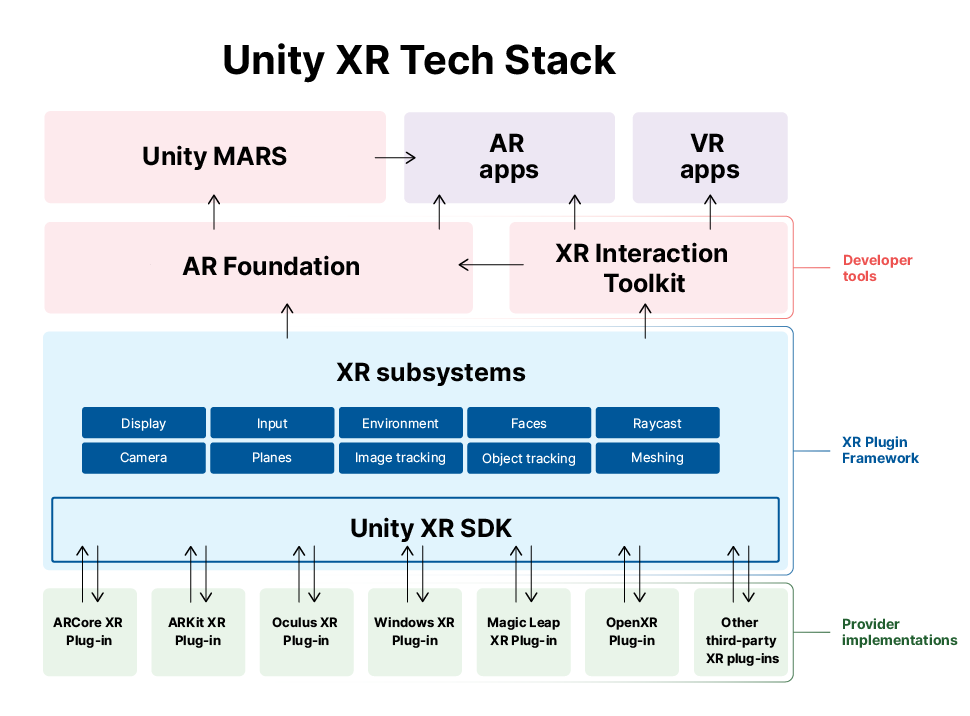
\includegraphics[width=0.8\textwidth]{figures/unity-xr-tech-stack.png}
	\caption{.}
	\label{fig:unity-xr-tech-stack}
\end{figure}

Oculus Quest as a standalone VR is great device for games and applications that need only baseline VR performance... When used for scientific visualization in standalone mode, the communication would have to be wireless and implemented with client-server architecture, which means the speed of sending data would deteriorate the usefulness of such application. It's still possible to use Oculus Quest for scientific visualization in VR, but it has to be connected to the powerful PC by special wire called Oculus Link, which is not part of the standard package. It has to be bought separately.

VR hardware like Oculus Rift, HTC Vive, PlayStationVR, and all Windows Mixed Reality headsets can be used for the high-performance visualization software, as the heavy computation is done by GPU on dedicated PC workstation.

% dopisat
Current software implementation was tested on Oculus Rift, HTC Vive and Oculus Quest with Link cable.

% upravit
Also, the augmented reality (AR) apps can be build from single codebase with Unity. Developers need to plan ahead and decide whether they want to target VR users, AR users or have the app be used by both device types (VR and AR). Usually, the term Mixed Reality is used to describe apps that target both types of devices. In this work, the focus was only on VR. Although in future, the AR looks as promising technology for specific usecases across scientific visualization, simulation and modeling industry. By leveraging Unity engine for the development of the visualization software for  this thesis, extending the software to support AR will be straightforward process.

Unity High Definition Render Pipeline (better for games, for simulation software not needed). \\

XR Interaction Toolkit - add interactivity to VR apps by dropping components into the scene. No need for coding the interaction scripts from scratch, developers can edit them for their own liking.

% trochu editovat (ne je to uplne odslova-doslova z Unity webu (https://docs.unity3d.com/Manual/SinglePassInstancing.html)
Single Pass Instanced rendering also known as Stereo Instancing, the GPU performs a single render pass, replacing each draw call with an instanced draw call. Thanks to this, the CPU usage is decreased heavily. Also the GPU usage is decreased thanks to the cache coherency between the two draw calls - significantly reduces power consumption of the VR application.

Windows and Linux (MacOS not supported) \\

Oculus Rift, Oculus Quest with Link cable, HTC Vive and Windows Mixed Reality headsets \\

\begin{figure}[!ht]
	\centering
	
\includegraphics[width=0.6\textwidth]{figures/empty.jpg}
	\caption{Native VR development with pre-packaged Unity scene.}
	\label{fig:unity-native-vr-dev}
\end{figure}

Setting up Oculus support in Unity

\begin{figure}[!ht]
	\centering
	
\includegraphics[width=0.6\textwidth]{figures/empty.jpg}
	\caption{Oculus support.}
	\label{fig:unity-oculus-support}
\end{figure}

Setting up HTC Vive support

\begin{figure}[!ht]
	\centering
	
\includegraphics[width=0.6\textwidth]{figures/empty.jpg}
	\caption{Oculus setup}
	\label{fig:unity-htc-support}
\end{figure}

\subsubsection{Interactivity}\label{sec:interactivity}

% dorobit + mozno premiestnit na spodok sekcie???
Natural way of interacting with the software has been for the long time through graphical user interfaces. Many programmers would still say that using terminal and learning the hotkeys for quicker work with the text and terminal window is much more effective than moving through the application interface with mouse. In fact, we could argue that GUIs helped to spread the software usage to more people and help them ... 

The conceptual move from 2D plane of our screens towards working immersed within 3D virtual world brings new challenges to the table. 
%-------------------------------------------

With the current technology, it's possible to not only use dedicated devices like hand controllers for using hands within virtual environments, but also hand tracking... %doplnit vetu?
%prepisat (copy-paste https://developer.oculus.com/documentation/unity/unity-handtracking/)
Hand tracking analyzes discrete hand poses and tracks the position of certain key points on your hands, such as knuckles or fingertips, in real time as your hands are moving. When you use hands as input, the hand’s pose drives a laser cursor-pointer that behaves like the standard controller cursor. You can use the cursor-pointer to highlight, select, click, or write your own app-level event logic. Integrated hands can perform object interactions by using simple hand gestures such as point, pinch, unpinch, scroll, and palm pinch.

Depending on your app’s input logic, you can use hands and controllers interchangeably. Hand tracking complements the Touch controllers and is not intended to replace controllers in all scenarios, especially with games or creative tools that require a high degree of precision. By opting-in to hand support, your app also needs to satisfy additional technical requirements specific to hand tracking for the Oculus store to accept it. To submit an app to Oculus Store, the app must support controllers along with hand tracking.

We support the use of hand tracking on Windows through the Unity editor, when using Oculus Quest + Oculus Link. 
% ------

%%%
% Native VR alebo VRTK Tilia??? Alebo Oculus Integration Package???
%%%

%To set up the interaction support across VR hardware, the appropriate scripts for each platform needs to be added and called in the application initialization part. For Oculus devices, the Oculus Integration Unity plugin provides \texttt{OVRInput.cs} script.
%
%For the controller haptics, Oculus provides \texttt{OVRHaptics.cs} script.


% upravit
It's often useful get the information about the physical variable !!!(nechat variable?)!!! in arbitrary part of the simulation. The most natural way to do that in VR is to point the finger, or in the case of hand controllers, pointing the hand interaction device to the part of running visualization. 

% dopisat
Application has to know where exactly the ray casted from the hand controller collided with the surface of the visualization object.  ... \ref{unity-pointer-interaction-code}.

\begin{lstlisting}[language=Rust, caption="Grab interaction code.", label=unity-pointer-interaction-code]
	public class Sim : MonoBehaviour
	{
		void Start()
		{
			// ...
			// ....
		}
		
		void PointerInteraction() {
			// ... rest of the code
			// ... rest of the code
			// ... rest of the code
			// ... rest of the code
			// ... rest of the code
			// ... rest of the code
		}
	}
\end{lstlisting}

% dopisat zrozumitelnejsie a rozsirit
After user points the hand controller or virtual hand to the visualization surface, information about the physical variables are shown within the VR environment (Figure~ \ref{fig:pointer-interaction}).

\begin{figure}[!ht]
	\centering
	\subfloat[Pointer interaction with hand controllers.\label{fig:pointer-interaction-hand-controllers}]{%
		
\includegraphics[width=0.45\textwidth]{figures/empty.jpg}%
	}\qquad
	\subfloat[Pointer interaction with virtual hands.\label{fig:pointer-interaction-hands}]{%
		
\includegraphics[width=0.45\textwidth]{figures/empty.jpg}%
	}
	\captionsetup{justification=centering}
	\caption{Information about the physical variables shown after user points to the specific part of the visualization.}
	\label{fig:pointer-interaction}
\end{figure}

% dopisat
Moving the objects in VR environment is done by hand controllers or with hands if the VR hardware supports it. 

General grabbing functionality ... \ref{unity-grab-interaction-code}.

\begin{lstlisting}[language=Rust, caption="Grab interaction code.", label=unity-grab-interaction-code]
	public class Sim : MonoBehaviour
	{
		void Start()
		{
			// ...
			// ....
		}
		
		void Interaction() {
			// ... rest of the code
			// ... rest of the code
			// ... rest of the code
			// ... rest of the code
			// ... rest of the code
			// ... rest of the code
		}
	}
\end{lstlisting}

The grabbing than can be performed by moving the hand controllers or virtual hands into the visualization object and clicking the appropriate buttons (or grabbing gesture) (Figure~ \ref{fig:grab-interaction}).

\begin{figure}[!ht]
	\centering
	
\includegraphics[width=0.6\textwidth]{figures/empty.jpg}
	\caption{Grab interaction.}
	\label{fig:grab-interaction}
\end{figure}

% dopisat
General zooming functionality ... \ref{unity-zoom-interaction-code}.

\begin{lstlisting}[language=Rust, caption="Zooming interaction code.", label=unity-zoom-interaction-code]
	public class Sim : MonoBehaviour
	{
		void Start()
		{
			// ...
			// ....
		}
		
		void Zooming() {
			// ... rest of the code
			// ... rest of the code
			// ... rest of the code
			// ... rest of the code
			// ... rest of the code
		}
	}
\end{lstlisting}



% --------------------------------------------------------------------

\subsection{Interactive Simulation}
% DONE
In this section, the implementation of interactive virtual reality visualization is presented. Unity game engine was picked as it provides an easy-to-use visual development environment with great support for VR baked-in. Their XR Plugin not only helped with VR development in current version of presented software, but offers a clear transition step towards supporting augmented reality in future.

VR user interface is also presented, showcasing different ways of how to interact with the running simulation. 


\subsubsection{Unity and Rust Interop}



% prepisat, zo stackoverflow (https://stackoverflow.com/questions/62232753/differences-between-a-pointer-and-a-reference-in-rust), niektore veci mozno prehodit do sekcie "Technology Stack" ----------
Use references when you can, use pointers when you must. If you're not doing FFI or memory management beyond what the compiler can validate, you don't need to use pointers.

Both references and pointers exist in two variants. There are shared references \& and mutable references \&mut. There are const pointers *const and mut pointers *mut (which map to const and non-const pointers in C). However, the semantics of references is completely different from the semantics of pointers.

References are generic over a type and over a lifetime. Shared references are written \&'a T in long form (where 'a and T are parameters). The lifetime parameter can be omitted in many situations. The lifetime parameter is used by the compiler to ensure that a reference doesn't live longer than the borrow is valid for.

Pointers have no lifetime parameter. Therefore, the compiler cannot check that a particular pointer is valid to use. That's why dereferencing a pointer is considered unsafe.

When you create a shared reference to an object, that freezes the object (i.e. the object becomes immutable while the shared reference exists), unless the object uses some form of interior mutability (e.g. using Cell, RefCell, Mutex or RwLock). However, when you have a const pointer to an object, that object may still change while the pointer is alive.

When you have a mutable reference to an object, you are guaranteed to have exclusive access to that object through this reference. Any other way to access the object is either disabled temporarily or impossible to achieve. For example:

\begin{lstlisting}
let mut x = 0;
{
	let y = &mut x;
	let z = &mut x; // ERROR: x is already borrowed mutably
	*y = 1; // OK
	x = 2; // ERROR: x is borrowed
}
x = 3; // OK, y went out of scope
\end{lstlisting}

Mut pointers have no such guarantee.

A reference cannot be null (much like C++ references). A pointer can be null.

Pointers may contain any numerical value that could fit in a usize. Initializing a pointer is not unsafe; only dereferencing it is.

If you have a *const T, you can freely cast it to a *const U or to a *mut T using as. You can't do that with references. However, you can cast a reference to a pointer using as, and you can "upgrade" a pointer to a reference by dereferencing the pointer (which, again, is unsafe) and then borrowing the place using \& or \&mut. For example:

\begin{lstlisting}
use std::ffi::OsStr;
use std::path::Path;

pub fn os_str_to_path(s: &OsStr) -> &Path {
	unsafe { &*(s as *const OsStr as *const Path) }
}
\end{lstlisting}

n C++, references are "automatically dereferenced pointers". In Rust, you often still need to dereference references explicitly. The exception is when you use the . operator: if the left side is a reference, the compiler will automatically dereference it (recursively if necessary!). Pointers, however, are not automatically dereferenced. This means that if you want to dereference and access a field or a method, you need to write (*pointer).field or (*pointer).method(). There is no -> operator in Rust.

% ------------------------

\begin{lstlisting}[language=Csharp, caption=., label=unity-rust-ffi-init-sim]
public class LBMAF
{
	private static IntPtr _sim_handle;
	private static IntPtr _data_handle;
	
	[DllImport("lbmaf")]
	private static extern bool init_sim(out IntPtr sim_handle, out IntPtr data_handle, UInt32 width, UInt32 height, float inflow_density, float inflow_ux, float omega, UInt32 obstacle_x, UInt32 obstacle_y, UInt32 obstacle_r);
	
	// C#/Unity interface with the Rust FFI
	public static bool InitSimulation(UInt32 w, UInt32 h, float rho0, float in_ux, float om, UInt32 obs_x, UInt32 obs_y, UInt32 obs_r)
	{
		return init_sim(out _sim_handle, out _data_handle, w, h, rho0, in_ux, om, obs_x, obs_y, obs_r);
	}
	// ... rest of the methods
}
\end{lstlisting}

% Multithreading
% - moving Array to thread,
% - read Array from multiple threada, 
% - write to Array from multiple threads,
% - write to single Array using Channel

\subsubsection{Visualizing Simulation Output in Real-Time}

First, on the Rust side, the data output from the LBM simulation has to be normalized to the range within minimum and maximum values (Listing \ref{rust-normalize}). 

\begin{lstlisting}[language=Rust, caption=Normalization of the simulation output., label=rust-normalize]
fn normalize(a: &Array<FloatNum>) -> Array<FloatNum> {
	let min = min_all(a).0;
	let max = max_all(a).0;
	(a - min) / (max - min) as FloatNum
}
\end{lstlisting}

% CPU-bound (Marshal.Copy)

This range is then color-coded to the rainbow colormap. Blue-ish colors denote slower velocities and red-ish colors faster velocities (Listing \ref{rust-colors-array}). Data representing information about color and opacity (alpha) of each pixel is ordered in $r$, $g$, $b$ and $a$ sub-arrays, then joined together and shuffled around to be correctly represented as Unity's Texture2D RGBA32 texture format.

\begin{lstlisting}[language=Rust, caption=Preparing the data output from Rust side of LBM simulation., label=rust-colors-array]
pub fn simulate(&mut self, inflow_density: FloatNum, inflow_ux: FloatNum, omega: FloatNum) {
	// ... code for actual computation
	
	results = normalize(&results);
	// Colormap for Unity's Texture2D (RGBA32)
	let r = flat(&((1.5f32 - abs(&(1.0f32 - 4.0f32 * (&results - 0.5f32)))) * 255));
	let g = flat(&((1.5f32 - abs(&(1.0f32 - 4.0f32 * (&results - 0.25f32)))) * 255));
	let b = flat(&((1.5f32 - abs(&(1.0f32 - 4.0f32 * &results))) * 255));
	let a = flat(&constant::<f32>(1.0 as FloatNum, self.dims));
	self.colors = flat(&transpose(&join_many(1, vec![&r, &g, &b, &a]), false)).cast::<u8>();
	
	// ... rest of the code
}

// Function for copying ArrayFire data to Rust's Vec
pub fn copy_colors_host(&mut self) {
	self.colors.host(self.results.as_mut_slice());
}
\end{lstlisting}

Second, on the Unity side

\begin{lstlisting}[language=Csharp, caption=The CPU-bound copying of the simulation results., label=unity-marshal-copy]
	public class LBMAF
	{
		private static IntPtr _sim_handle;
		private static IntPtr _data_handle;
		
		[DllImport("lbmaf")]
		private static extern bool init_sim(out IntPtr sim_handle, out IntPtr data_handle, UInt32 width, UInt32 height, float inflow_density, float inflow_ux, float omega, UInt32 obstacle_x, UInt32 obstacle_y, UInt32 obstacle_r);
		
		// C#/Unity interface with the Rust FFI
		public static bool InitSimulation(UInt32 w, UInt32 h, float rho0, float in_ux, float om, UInt32 obs_x, UInt32 obs_y, UInt32 obs_r)
		{
			return init_sim(out _sim_handle, out _data_handle, w, h, rho0, in_ux, om, obs_x, obs_y, obs_r);
		}
		// ... rest of the methods
	}
\end{lstlisting}

% GPU-bound (OpenGL and OpenCL interop)
The faster alternative to CPU-bound data copying is to work only within context of the GPU, since we already have the data residing there after doing computations for LBM simulation. The easiest way to do this is to leverage OpenCL and OpenGL interoperability. \citep{malcolmArrayFireGPUAcceleration2012}
 
OpenCL-OpenGL sharing works in a very particular way. The OpenCL context that needs to be shared with an OpenGL context has to be created using an OS specific OpenGL context handle as one of it's context properties. The OpenGL context used by ArrayFire's OpenCL-OpenGL shared context is completely different from the OpenGL context that Unity uses.

As for such attempts trying to use ArrayFire's OpenGL context for copying data from OpenCL Arrays to Unity's OpenGL texture, common error usually pops up:

\begin{lstlisting}
Error executing function: clCreateFromGLTexture2D  
Status error code: CL_INVALID_CONTEXT (-34)  
\end{lstlisting}

First, a workaround has to be implemented prior to doing any work with external OpenGL context. Simply put, ArrayFire has to switch to this context and use it. Workaround procedure consists of the following:

\begin{enumerate}
	\item Pick the device you want to do OpenCL-OpenGL sharing on and create a \texttt{ocl_device_id} handle using fuctions from the\texttt{ocl} Rust create.
	\item Now, for this device from step (1), create a new OpenGL context, passing the properties specific to your OS as an arguments for the creation function.
	\item Create an OpenCL queue for this device in newly created OpenCL-OpenGL shared context.
	\item Now add this context to ArrayFire device manager using \texttt{afcl::add_device_context}.
	\item Finally, set this device/context queue as your ArrayFire device using \texttt{set_device_context()}.
\end{enumerate}

All of these has to be completed before any ArrayFire computations are carried out so that you don't have buffers that are created on a different OpenCL context. Only after this initial procedure, the creation of a shared OpenCL-OpenGL buffer that is then used for direct memory copying to the Unity's OpenGL texture is then possible. ArrayFire shall assume control of shared OpenCL-OpenGL buffer to take care of ownership, only this way it can operate on shared OpenCL memory. For such case ArrayFire provides 
\texttt{Array.lock()} and \texttt{Array.unlock()} functions.

Implementing OpenGL-OpenCL interoperability with ArrayFire and Unity isn't straightforward and involves additional help from the ArrayFire developers. Although it is documented for simple windowing platforms that use OpenGL textures for drawing to the screen, it's much more complex within the setting of this work, such as implementing interoperability with Unity game engine. On the other note, OpenGL support in virtual reality headsets that use cable connection to PC workstations (setting currently needed for having access to powerful GPUs) is very limited. Therefore it was not successfully implemented in current work. 

Still, it is of very high importance to implement GPU-bound visualization techniques into the future versions of LBM solver, though. When dealing with complex 3D simulation, multiple-relaxation time algorithm and more directions of particle distribution function within the lattice node, CPU-bound visualization could easily become a bottle neck.

\subsubsection{Setting Initial Conditions}

Before starting a simulation, user is encouraged to configure the initial parameters that are then sent to the simulation software which uses them for setting the simulation's initial boundary conditions and underlying physics for specified model. Default parameters are provided for the user, so if nothing is changed, D2Q9-LBM simulation of Kármán vortex street on 300x100 grid is initialized, with initial conditions of inflow density $\rho = 1.0$, inflow speed $\bm{u}_x = 0.1$ and Reynolds number $Re = 220$.

The physics and lattice parameters can be set in Unity Editor and also inside the virtual reality environment.

In development phase, these parameters are available as a part of the simulation script interface. The inputs are generated automatically for each public variable in script's class (Listing \ref{unity-public-variables-editor}).

\begin{lstlisting}[language=Rust, caption=Boundary conditions at solid nodes., label=unity-public-variables-editor]
	public class Sim : MonoBehaviour
	{
		public UInt32 width = 0;
		public UInt32 height = 0;
		private Texture2D image;
		
		void Start()
		{
			image = new Texture2D(width, height, TextureFormat.RGBA32, false);
			GetComponent<Renderer>().material.mainTexture = image;
		}
		
		// ... rest of the code
	}
\end{lstlisting}

When looking into the Unity Editor, the script interface now has two numerical inputs, \texttt{width} and \texttt{height} (Figure~ \ref{fig:unity-script-interface-public-vars}).

\begin{figure}[!ht]
	\centering
	
\includegraphics[width=0.6\textwidth]{figures/empty.jpg}
	\caption{Unity Editor with script interface.}
	\label{fig:unity-script-interface-public-vars}
\end{figure}




\subsubsection{Updating Boundary Conditions}

\begin{lstlisting}[language=Rust, caption=".", label=]
#[no_mangle]
pub extern "C" fn simulate(
	ptr: *mut Sim,
	inflow_density: FloatNum,
	inflow_ux: FloatNum,
	omega: FloatNum
) {
	if !ptr.is_null() {
		Sim::from_ptr(ptr).simulate(inflow_density, inflow_ux, omega);
	}
}
\end{lstlisting}

\begin{lstlisting}[language=Csharp, caption=".", label=]
	#[no_mangle]
	pub extern "C" fn simulate(
	ptr: *mut Sim,
	inflow_density: FloatNum,
	inflow_ux: FloatNum,
	omega: FloatNum
	) {
		if !ptr.is_null() {
			Sim::from_ptr(ptr).simulate(inflow_density, inflow_ux, omega);
		}
	}
\end{lstlisting}

\subsubsection{Time Manipulation}

Visualization is running continuously throughout the simulation in parallel to the actual computations. It's sometimes good to pause the running simulation when there's something interesting to investigate or explore in more detail.

% editovat aby to znelo lepsie
For simple pausing and continuing the simulation, the VR interface contains a GUI for that (Figure~ \ref{fig:unity-pause-play}).

\begin{figure}[!ht]
	\centering
	
\includegraphics[width=0.6\textwidth]{figures/empty.jpg}
	\caption{Interface for controlling the state of simulation.}
	\label{fig:unity-pause-play}
\end{figure}

Implementation of the co-routine starting, pausing and stopping is implemented in Listing \ref{unity-start-stop-coroutine}.

\begin{lstlisting}[language=Rust, caption="Starting\, pausing and stopping the co-routines in Unity.", label=unity-start-stop-coroutine]
	public class Sim : MonoBehaviour
	{
		void Start()
		{
			// ...
			StartCoroutine("StartSimulation")
		}
		
		IEnumerate StartSimulation() {
			// ... rest of the code
		}
	}
\end{lstlisting}

% editovat aby to znelo lepsie
To manipulate time and go back in history, the simulation data has to be stored to the disk. Each second, XY GB of data is stored. 

To go back in time, user can use the slider and move the knob backward or forward (Figure~ \ref{fig:unity-time-manipulation}).

\begin{figure}[!ht]
	\centering
	
\includegraphics[width=0.6\textwidth]{figures/empty.jpg}
	\caption{Interface for controlling the state of simulation.}
	\label{fig:unity-time-manipulation}
\end{figure}

% ----------------------------------------------------------------

\subsection{Performance Analysis}\label{perf-analysis}
% DONE
The performance of computers used for scientific applications are commonly measure in floating point operations per second (FLOPS), which represents the time it takes for multiplying two 32 or 64 bit floating-point numbers.

At the time of writing, the fastest supercomputer in the world runs at roughly 440 PetaFLOPS ($440\times10^{15}$). The next milestone in computer engineering is to build a supercomputer capable of running at speeds exceeding 1 ExaFLOPS ($10^{18}$). In contrast to HPC systems, the fastest GPU on consumer market, at the time of writing, is NVIDIA's GeForce RTX 3090 that peaks at 35 TeraFLOPS.

Performance of LBM simulations is measured in ``Million Lattice Updates Per Second" (MLUPS), which is a standard unit of measurement within the LBM research community. It states that the simulation code updates a computational domain of million cells in lattice during one CPU second. The same metric is used for both single and double-precision floating-point operations in benchmarked simulations. 

\subsubsection{Hardware}\label{sec:hardware-gpus}
% DONE
Since ArrayFire allows for using not only GPU backends but also CPU, we added a CPU benchmarks executed on Intel Core i7 6800K running at 3.40GHz. Performance peaked at around 19 MLUPS and stayed the same between various domain sizes across both academic test cases.

Most of the GPU benchmarks were done using both CUDA and OpenCL backends, although differences between them were minimal. Therefore in following tables and graphical representations of the data, we show MLUPS numbers solely from OpenCL benchmarks, since testing on this platform allowed us to perform benchmarks not only on NVIDIA hardware, but also on AMD GPU.

We tested the solver performance on 4 different GPUs. The AMD Radeon R9 M370X is of mobile GPU type installed in laptops. In the current study, the AMD GPU was tested on the higher-end Macbook Pro 2015. The NVIDIA GTX 1070 is the average desktop GPU and its price at the time of writing this article is \$443.78 USD according to PassMark G3D Mark (a GPU benchmarking website). The NVIDIA RTX 3090 is a top-of-the-line, consumer-grade, enthusiast-level GPU with the price of \$2139.99 USD according to PassMark G3D Mark at the time of writing. Also, to test the performance across multiple architectures of NVIDIA GPU cards, we added a NVIDIA GeForce RTX 2080 Ti to the suite of benchmarks.

\begin{table*}[!ht]
	\centering\small
	{\renewcommand{\arraystretch}{1.1}%
		{\setlength{\tabcolsep}{0.4em}
	\begin{tabular}{ |p{4.3cm}||p{2.1cm}|p{2.2cm}|p{2.2cm}|p{2.5cm}| }
		\hline
		& R9 M370X \newline(AMD) & GTX 1070 \newline(NVIDIA) & RTX 2080 Ti \newline(NVIDIA) & RTX 3090 \newline(NVIDIA) \\
		\hline
		Architecture   & GCN 1.0 & Pascal  & Turing &  Ampere  \\
		\hline
		Number of cores (CU/SM)   & 640 (10 CU) & 1920~(15~SM)   &  4352 (68 SM) &  10496 (82 SM) \\
		\hline
		Peak f32 perf. (TFLOPS)   & 1.024  & 6.463  & 13.45 &  35.58 \\
		\hline
		Memory clock (MHz)   & 1125  & 2002   & 1750 &   1219 \\
		\hline
		Memory bandwidth (GB/s)   & 72.00  & 256.3   & 616.0 &   936.2 \\
		\hline
		L1 cache size (KB)   & 16  & 48   & 64 &   128 \\
		\hline
	\end{tabular}}}
	\caption{GPU hardware specifications. These were used for benchmarking the LBM simulation software described in this work (taken from \url{https://www.techpowerup.com/gpu-specs/}). SM - streaming multiprocessor, CU - computing units.}
	\label{tab:gpus}
\end{table*}

\subsubsection{Results}

In 2D lid-driven cavity test, benchmarks showed great results with significant speedup compared to CPU backend (Table \ref{tab:lid-mlups-all-2d}).

\begin{table}[!ht]
	\centering\small
	{\renewcommand{\arraystretch}{1.1}%
		{\setlength{\tabcolsep}{0.5em}
	\begin{tabular}{ |p{2.7cm}||p{2.2cm}|p{2.2cm}|p{2.4cm}|p{2.1cm}|  }
		\hline
		Domain & R9 M370X & GTX~1070 & RTX~2080~Ti & RTX 3090 \\
		\hline
		64$\times$64   & 23 & 40  & 11  & 55  \\
		\hline
		128$\times$128   & 59 & 226  & 50   & 225  \\
		\hline
		256$\times$256   & 97 & 675  & 186   & 868  \\
		\hline
		512$\times$512   & 120 & 1006  & 600   & 2890  \\
		\hline
		1024$\times$1024   & 111 & 1143   & 1401   & 4620  \\
		\hline
		2048$\times$2048   & - & 1200  & 2195  & 5465  \\
		\hline
		4096$\times$4096   & - & -  & 2394  & 5730  \\
		\hline
	\end{tabular}}}
	\caption{Peak MLUPS of lid-driven cavity test case in 2D. The data represents single-precision floating point computation (taking only the steady performance after initial warm-up and removal of sudden spikes).}
	\label{tab:lid-mlups-all-2d}
\end{table}

Single floating-point (f32) calculations perform significantly faster than double-precision (f64). The difference between f32 and f64 computation is the doubling of the problem data size. ArrayFire's Array objects are typed, i.e. syntactic construction of a f32 type array looks different from f64 array. It's not hidden in any fashion. In fact, the programmer needs to know what type they are using as performance on accelerators (GPUs) is not the same for all types, scalar or vector types. Type dictates the size of memory on the GPU that will be used, and hence the amount of bandwidth that can be utilized during data transfers. Usually similar sized types have similar data transfer characteristics. Doubles are theoretically expected to have half the performance given by Floats. This difference can be seen in D2Q9 lid-driven cavity and Kármán vortex test cases (Figure~\ref{fig:d2q9_lid_mlups_f32} ,\ref{fig:d2q9_lid_mlups_f64}, \ref{fig:d2q9_channel_mlups_f32}, \ref{fig:d2q9_channel_mlups_f64}, but it's manifesting much better in D3Q27-MRT lid-driven cavity benchmarks (Figure~\ref{fig:d3q27_lid_mlups_f32} ,\ref{fig:d3q27_lid_mlups_f64}).

\begin{figure}[!ht]
	\centering
	\subfloat[Performance on Radeon R9 M370X GPU.\label{fig:d2q9_lid_mlup_r9_32bit}]{%
		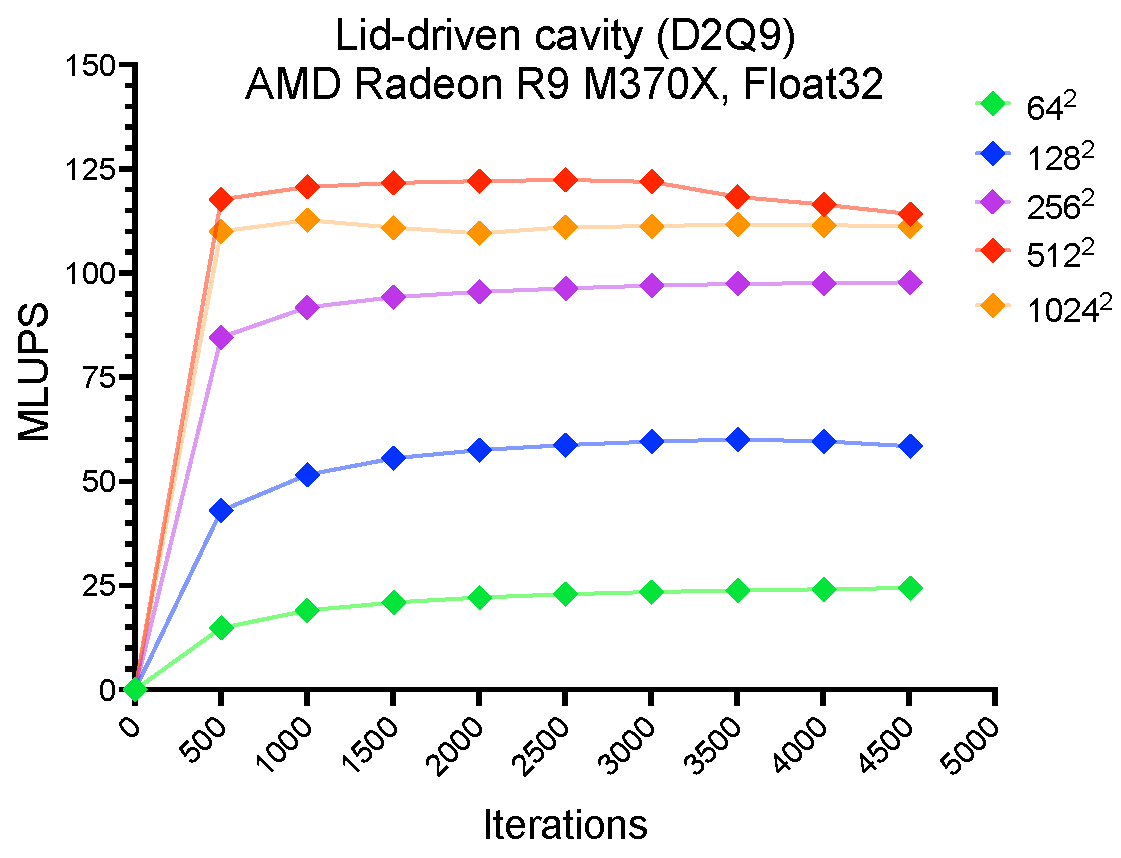
\includegraphics[width=0.45\textwidth]{data/r9_32bit_d2q9_bgk_lid_mlups.pdf}%
	}\qquad
	\subfloat[Performance on GTX 1070 GPU.\label{fig:d2q9_lid_mlup_gtx1070_32bit}]{%
		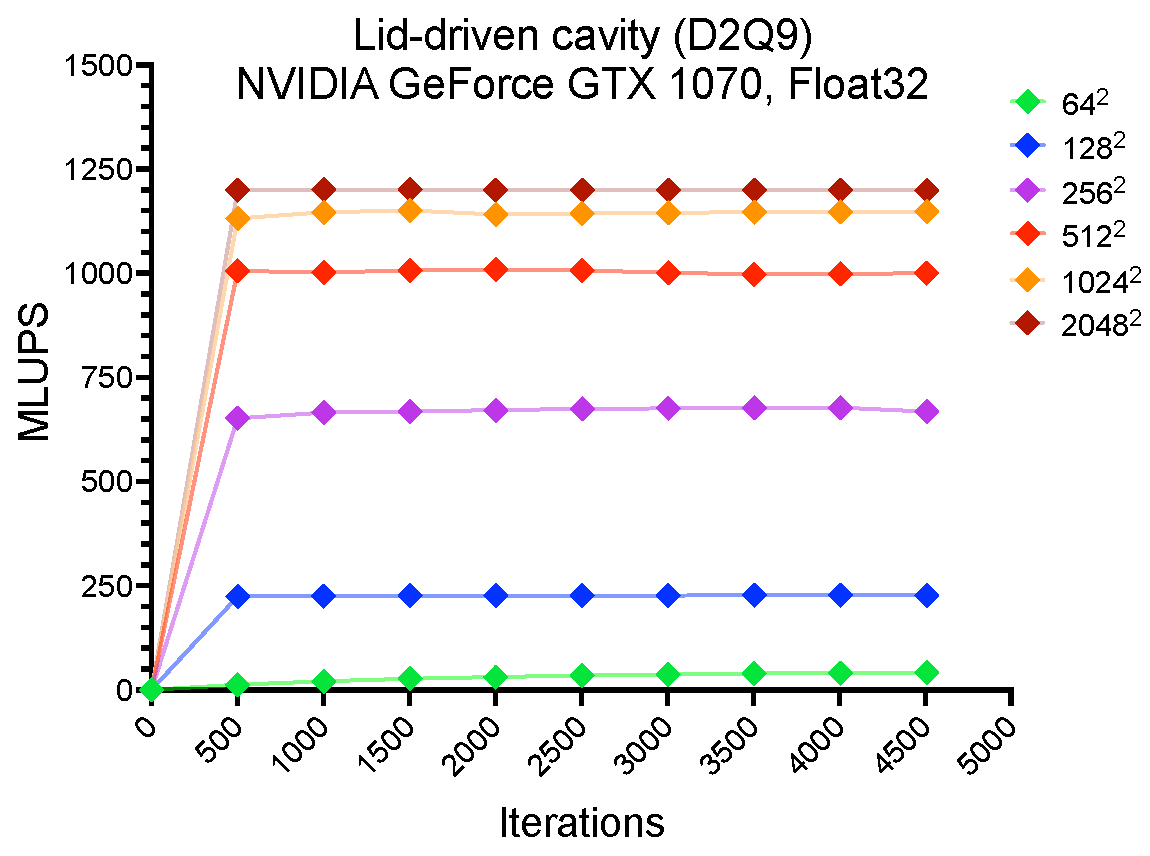
\includegraphics[width=0.45\textwidth]{data/gtx1070_32bit_d2q9_bgk_lid_mlups.pdf}%
	}\qquad
	\subfloat[Performance on RTX 2080 Ti GPU.\label{fig:d2q9_lid_mlups_rtx2080ti_32bit}]{%
		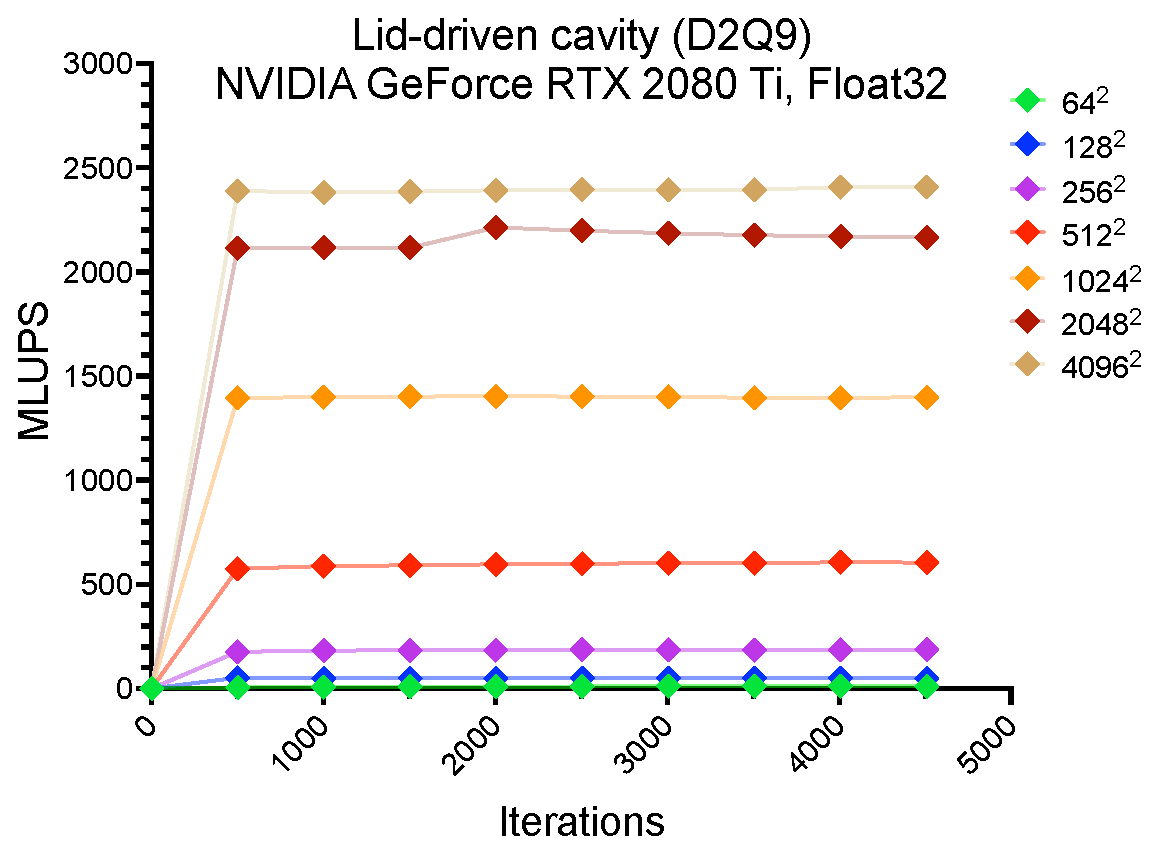
\includegraphics[width=0.45\textwidth]{data/rtx2080ti_32bit_d2q9_bgk_lid_mlups.pdf}%
	}\qquad
	\subfloat[Performance on RTX 3090 GPU.\label{fig:d2q9_lid_mlup_rtx3090_32bit}]{%
		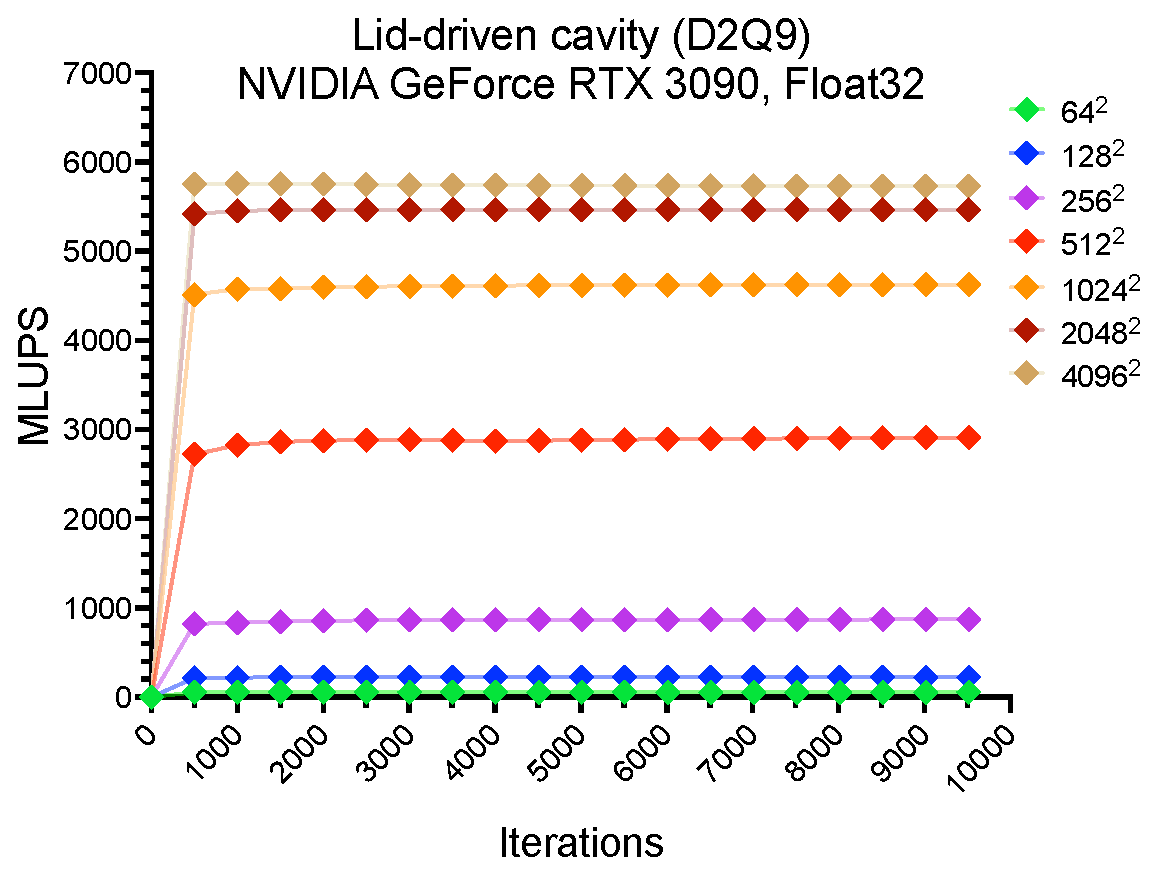
\includegraphics[width=0.45\textwidth]{data/rtx3090_32bit_d2q9_bgk_lid_mlups.pdf}%
	}
	\captionsetup{justification=centering}
	\caption{Single-precision performance analysis of 2D lid-driven cavity on D2Q9 stencil.}
	\label{fig:d2q9_lid_mlups_f32}
\end{figure}

\begin{figure}[!ht]
	\centering
	\subfloat[Performance on Radeon R9 M370X GPU.\label{fig:d2q9_lid_mlup_r9_64bit}]{%
		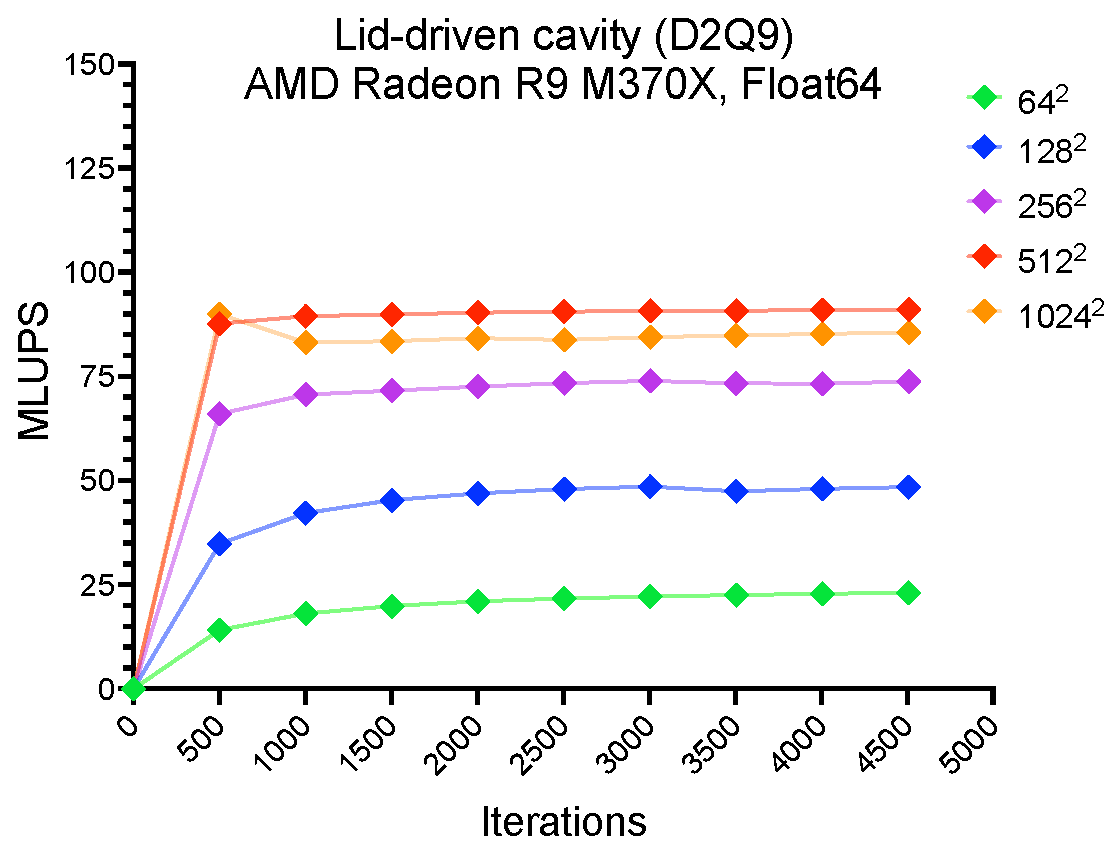
\includegraphics[width=0.45\textwidth]{data/r9_64bit_d2q9_bgk_lid_mlups.pdf}%
	}\qquad
	\subfloat[Performance on GTX 1070 GPU.\label{fig:d2q9_lid_mlup_gtx1070_64bit}]{%
		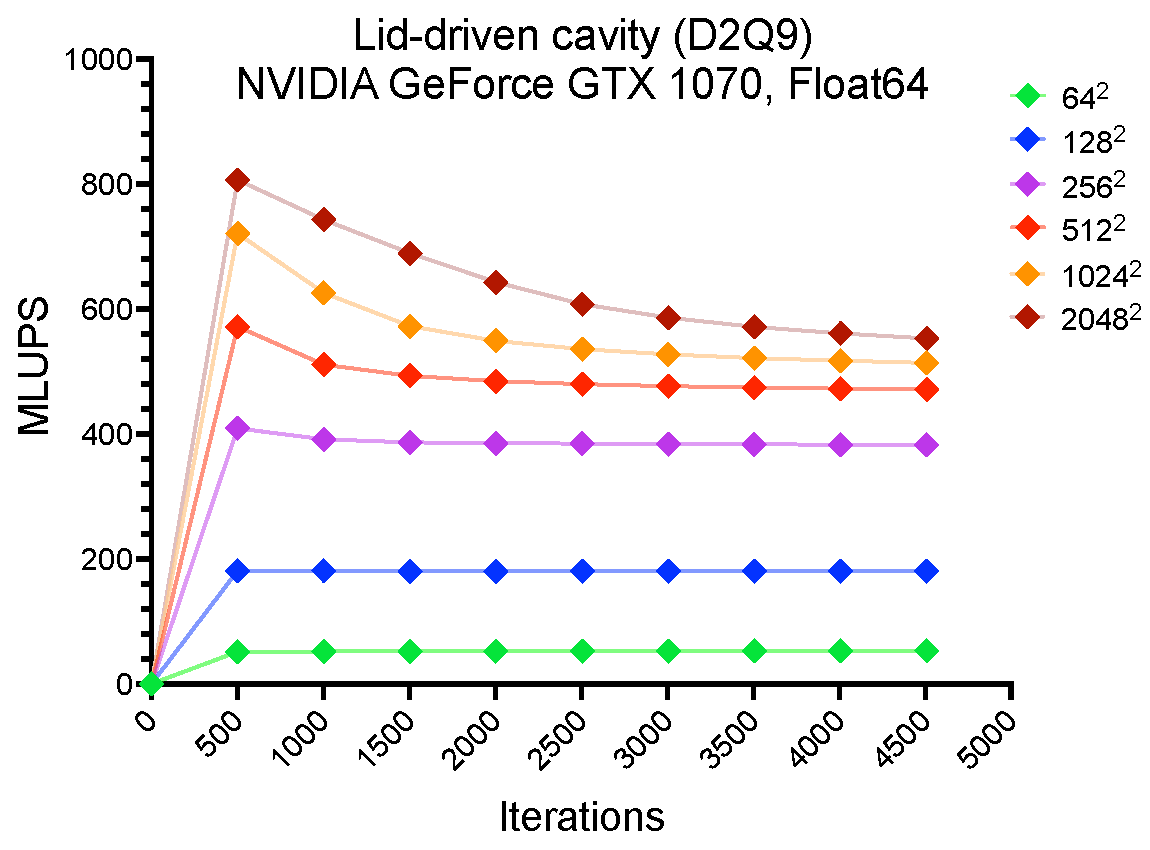
\includegraphics[width=0.45\textwidth]{data/gtx1070_64bit_d2q9_bgk_lid_mlups.pdf}%
	}\qquad
	\subfloat[Performance on RTX 2080 Ti GPU.\label{fig:d2q9_lid_mlups_rtx2080ti_64bit}]{%
		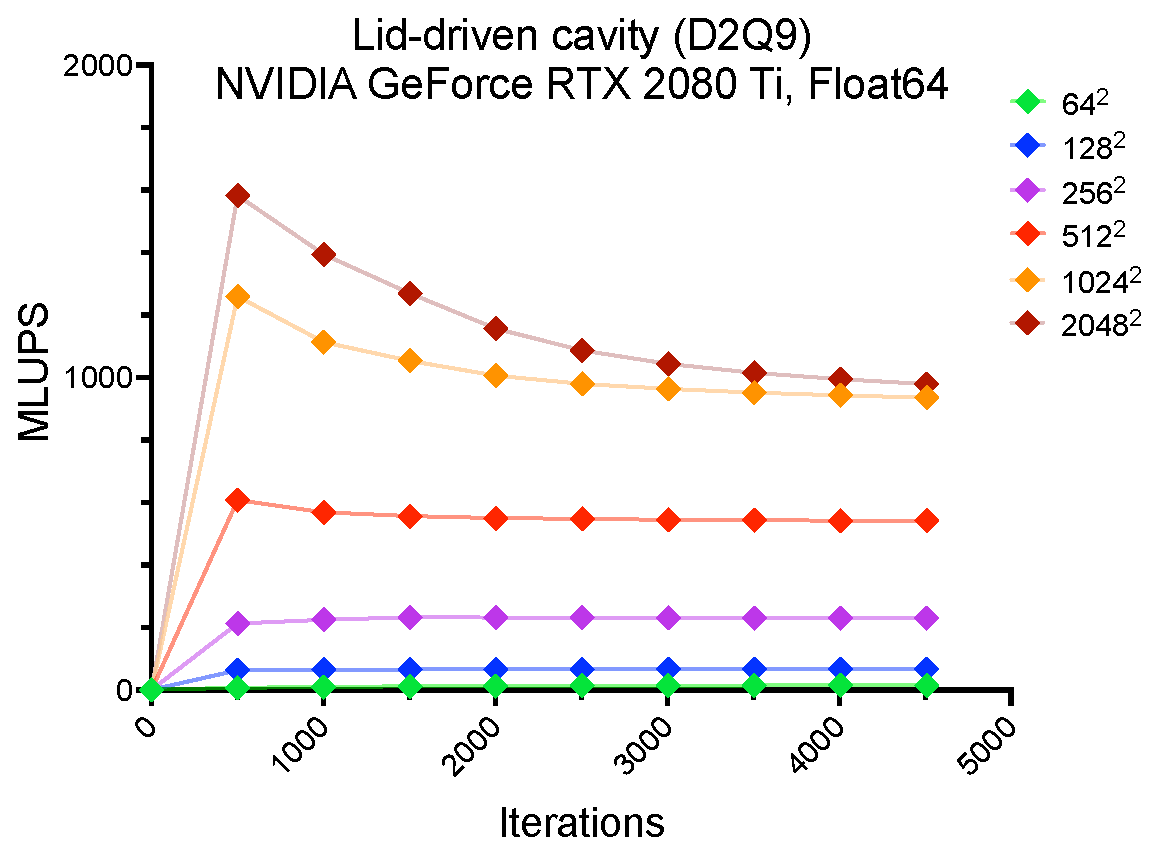
\includegraphics[width=0.45\textwidth]{data/rtx2080ti_64bit_d2q9_bgk_lid_mlups.pdf}%
	}\qquad
	\subfloat[Performance on RTX 3090 GPU.\label{fig:d2q9_lid_mlup_rtx3090_64bit}]{%
		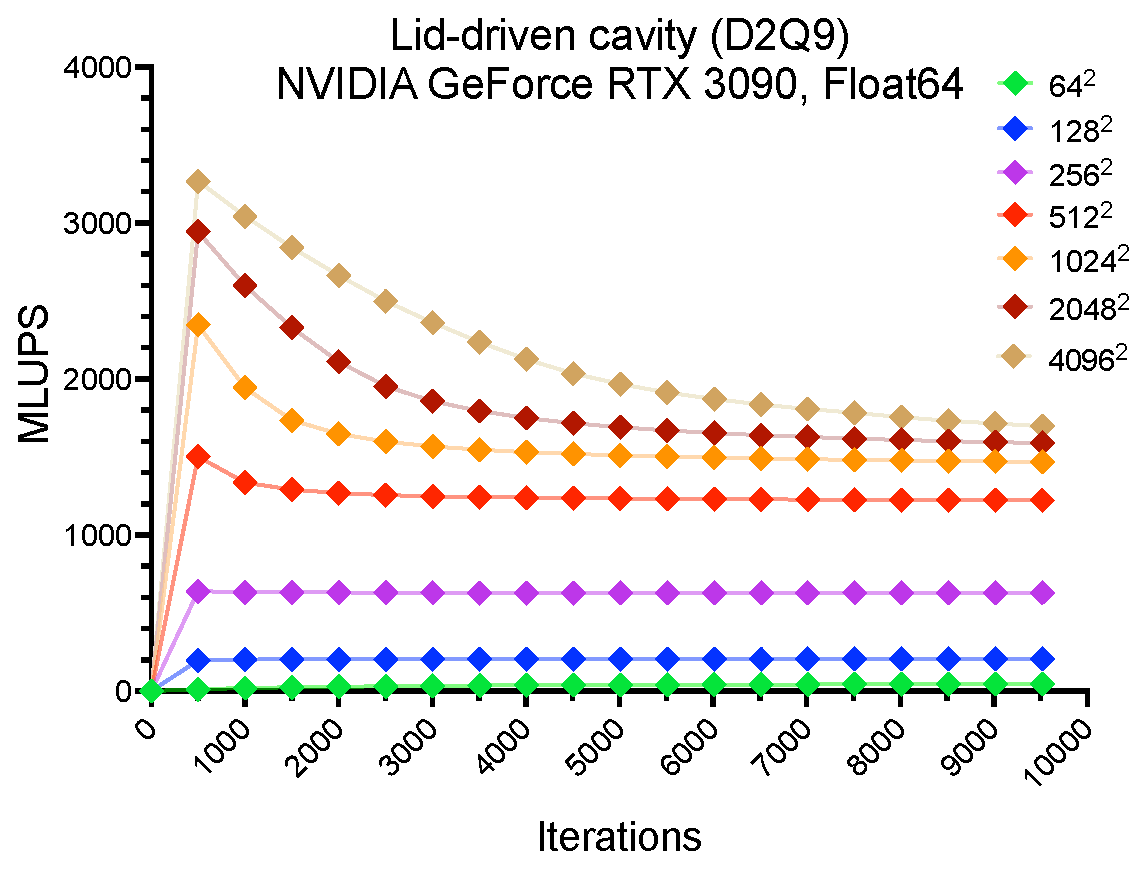
\includegraphics[width=0.45\textwidth]{data/rtx3090_64bit_d2q9_bgk_lid_mlups.pdf}%
	}
	\captionsetup{justification=centering}
	\caption{Double-precision performance analysis of 2D lid-driven cavity on D2Q9 stencil.}
	\label{fig:d2q9_lid_mlups_f64}
\end{figure}

For the 2D Kármán vortex test case, benchmarks showed similar results (\ref{tab:channel-mlups}). The performance spikes in so-called "warm-up" phase at the start of simulation were less significant in double-precision benchmarks than in lid-driven cavity test. 

\begin{table}[!ht]
	\centering\small
	{\renewcommand{\arraystretch}{1.1}%
		{\setlength{\tabcolsep}{0.5em}
	\begin{tabular}{ |p{2.7cm}||p{2.2cm}|p{2.2cm}|p{2.4cm}|p{2.21cm}|  }
		\hline
		Domain & R9 M370X & GTX~1070 & RTX~2080~Ti & RTX 3090 \\
		\hline
		300$\times$100   & 73 & 340 & 361    & 361  \\
		\hline
		420$\times$150   & 93 & 627 & 122    & 740  \\
		\hline
		600$\times$200   & 107 & 810 & 180    & 1343  \\
		\hline
		1000$\times$300   & 123 & 1007 & 325    & 3000  \\
		\hline
		1500$\times$400   & 117 & 1100 & 731    & 4055  \\
		\hline
		2000$\times$500   & 130 & 1140 & 1010    & 4510  \\
		\hline
		3000$\times$1000   & 113 & 1175 & 1311    & 5313  \\
		\hline
		4200$\times$1500   & - & 1194 & 2016    & 5557  \\
		\hline
		6000$\times$2000   & - & - & 2522  & 5670  \\
		\hline
		10000$\times$3000   & - & - & -   & 5720  \\
		\hline
	\end{tabular}}}
	\caption{Peak MLUPS of 2D Kármán vortex street test case with BGK collision operator. The data represents single-precision floating point computation (taking only the steady performance after initial warm-up and removal of sudden spikes).}
	\label{tab:channel-mlups}
\end{table}


\begin{figure}[!ht]
	\centering
	\subfloat[Performance on Radeon R9 M370X GPU.\label{fig:d2q9_channel_mlup_r9_32bit}]{%
		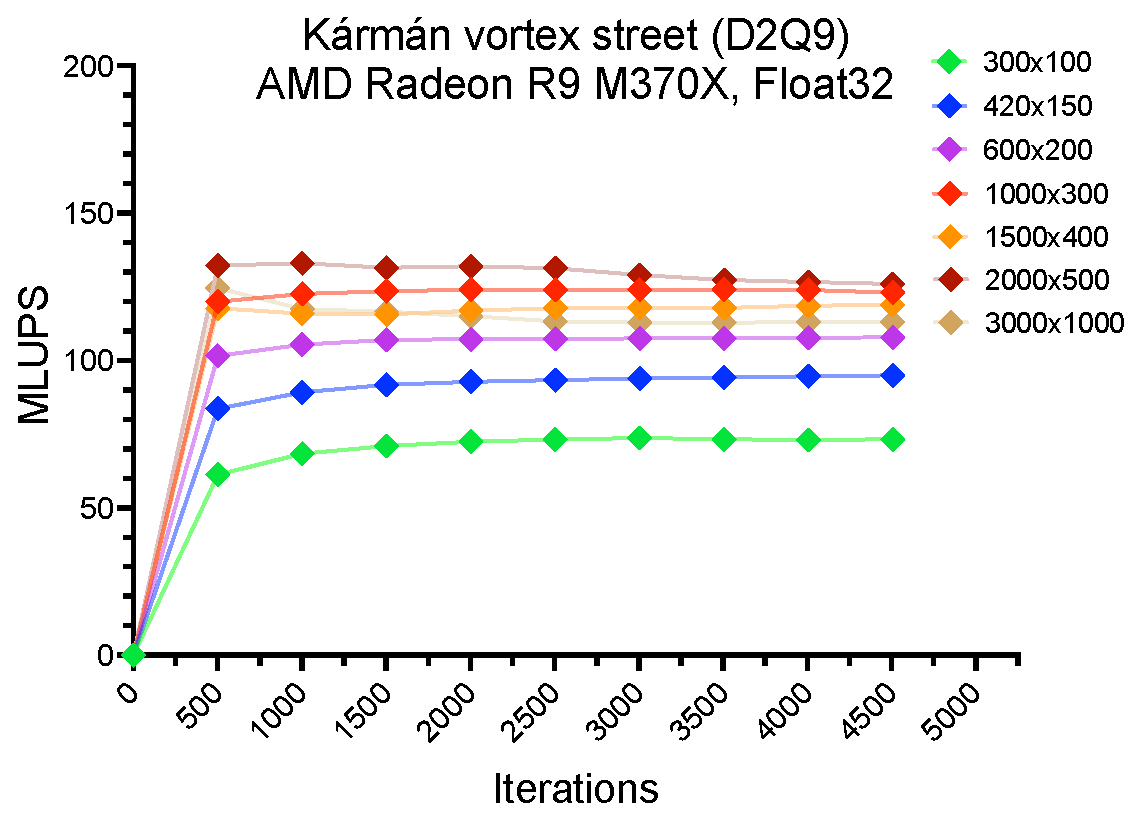
\includegraphics[width=0.45\textwidth]{data/r9_32bit_d2q9_bgk_channel_mlups.pdf}%
	}\qquad
	\subfloat[Performance on GTX 1070 GPU.\label{fig:d2q9_channel_mlup_gtx1070_32bit}]{%
		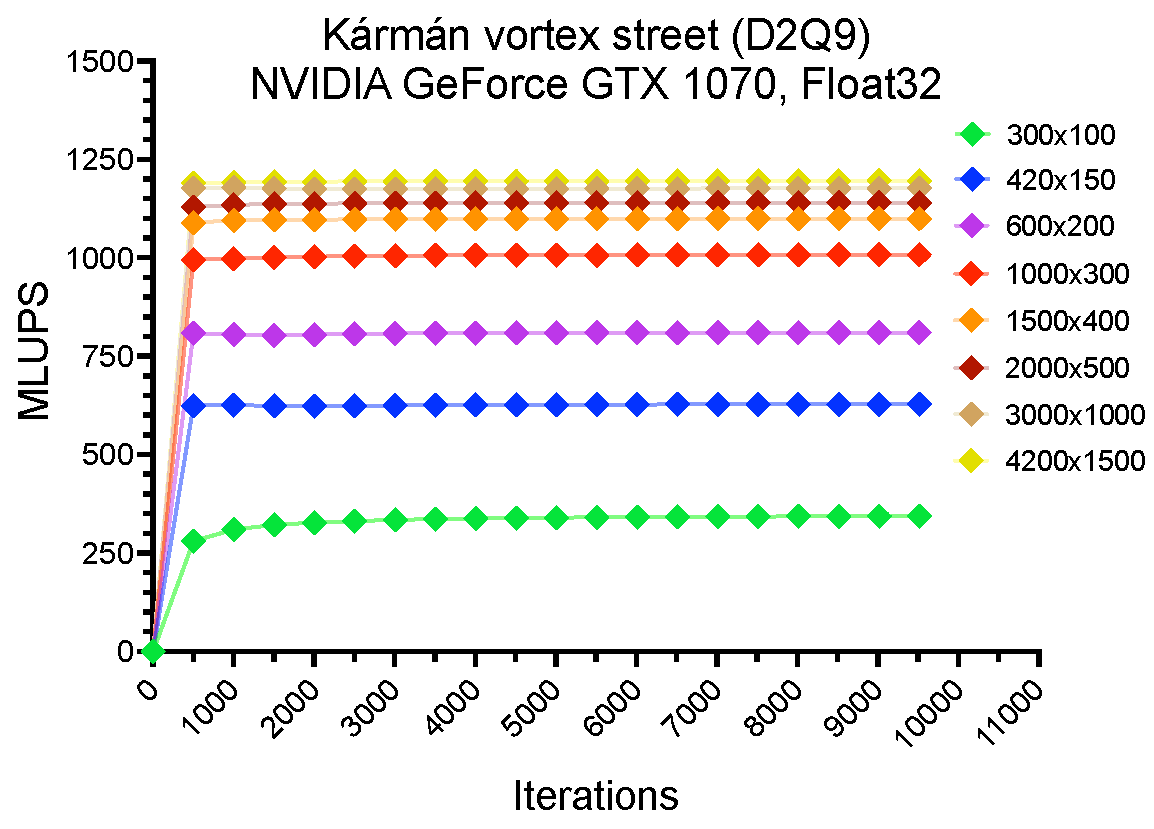
\includegraphics[width=0.45\textwidth]{data/gtx1070_32bit_d2q9_bgk_channel_mlups.pdf}%
	}\qquad
	\subfloat[Performance on RTX 2080 Ti GPU.\label{fig:d2q9_channel_mlups_rtx2080ti_32bit}]{%
		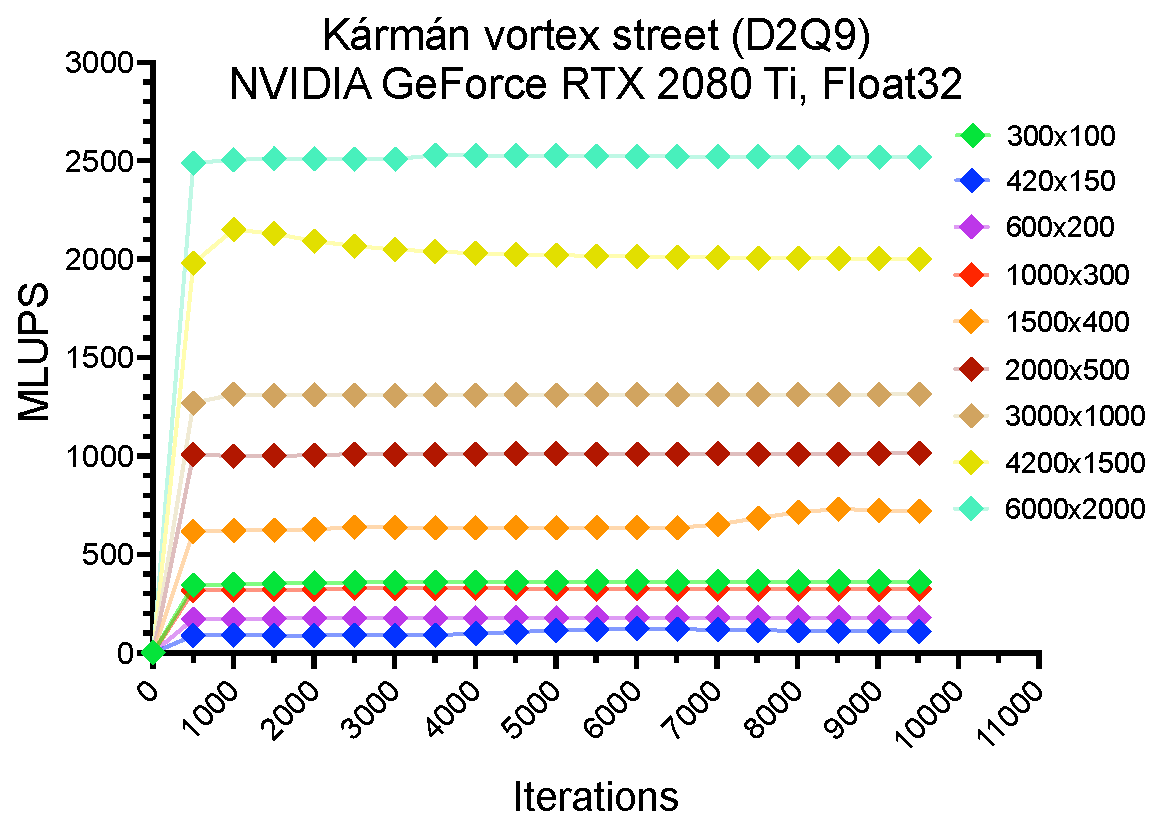
\includegraphics[width=0.45\textwidth]{data/rtx2080ti_32bit_d2q9_bgk_channel_mlups.pdf}%
	}\qquad
	\subfloat[Performance on RTX 3090 GPU.\label{fig:d2q9_channel_mlup_rtx3090_32bit}]{%
		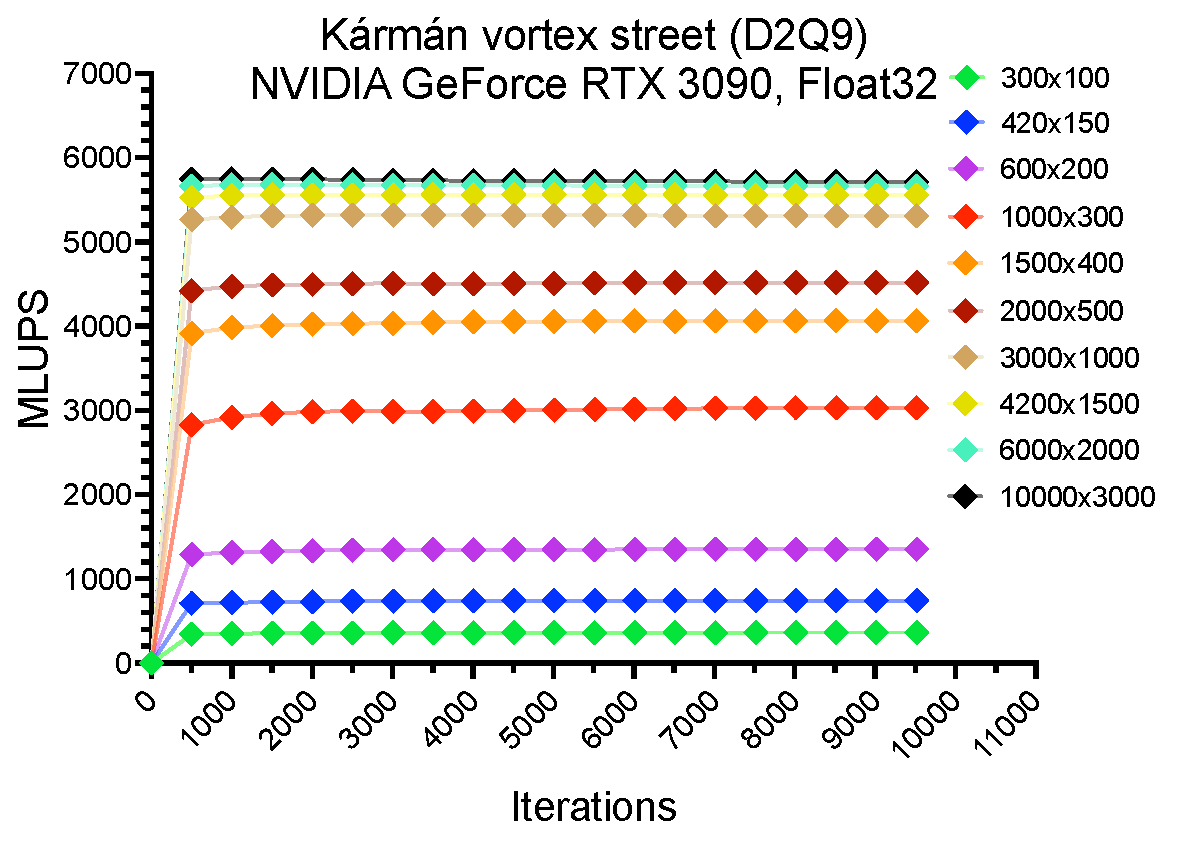
\includegraphics[width=0.45\textwidth]{data/rtx3090_32bit_d2q9_bgk_channel_mlups.pdf}%
	}
	\captionsetup{justification=centering}
	\caption{Single-precision performance analysis of 2D Kármán vortex on D2Q9 stencil.}
	\label{fig:d2q9_channel_mlups_f32}
\end{figure}


\begin{figure}[!ht]
	\centering
	\subfloat[Performance on Radeon R9 M370X GPU.\label{fig:d2q9_channel_mlup_r9_64bit}]{%
		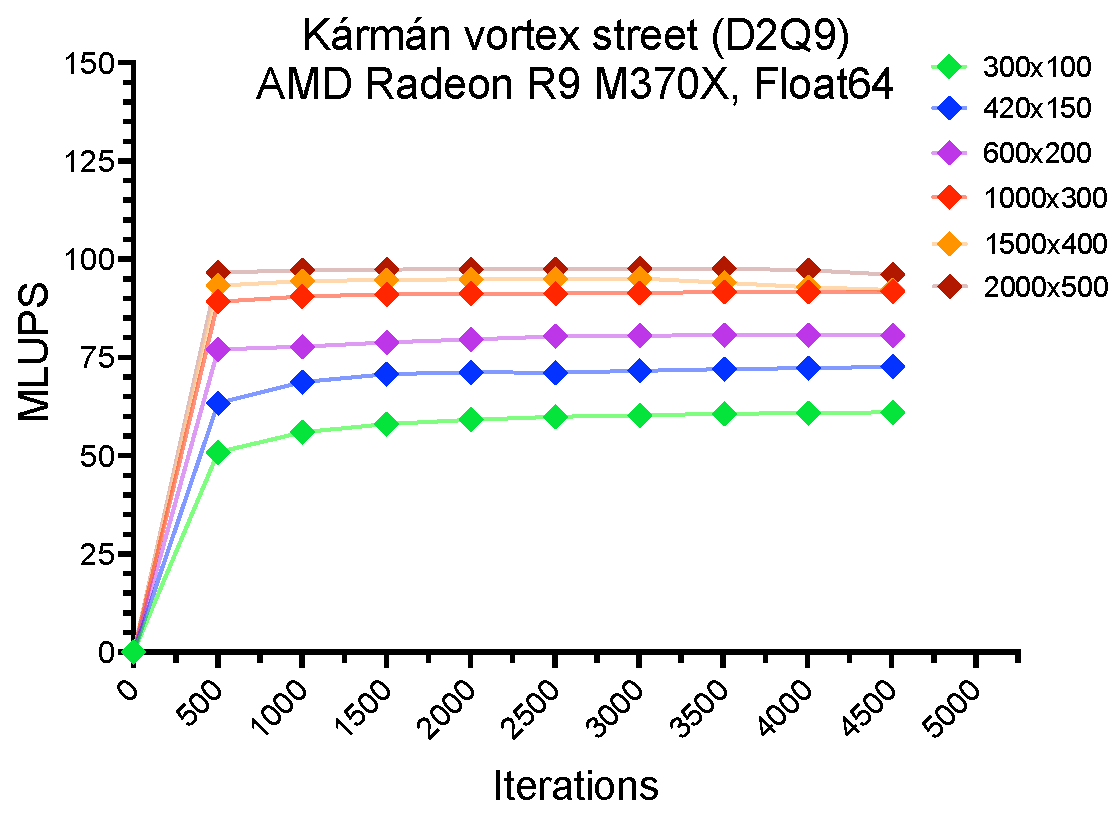
\includegraphics[width=0.45\textwidth]{data/r9_64bit_d2q9_bgk_channel_mlups.pdf}%
	}\qquad
	\subfloat[Performance on GTX 1070 GPU.\label{fig:d2q9_channel_mlup_gtx1070_64bit}]{%
		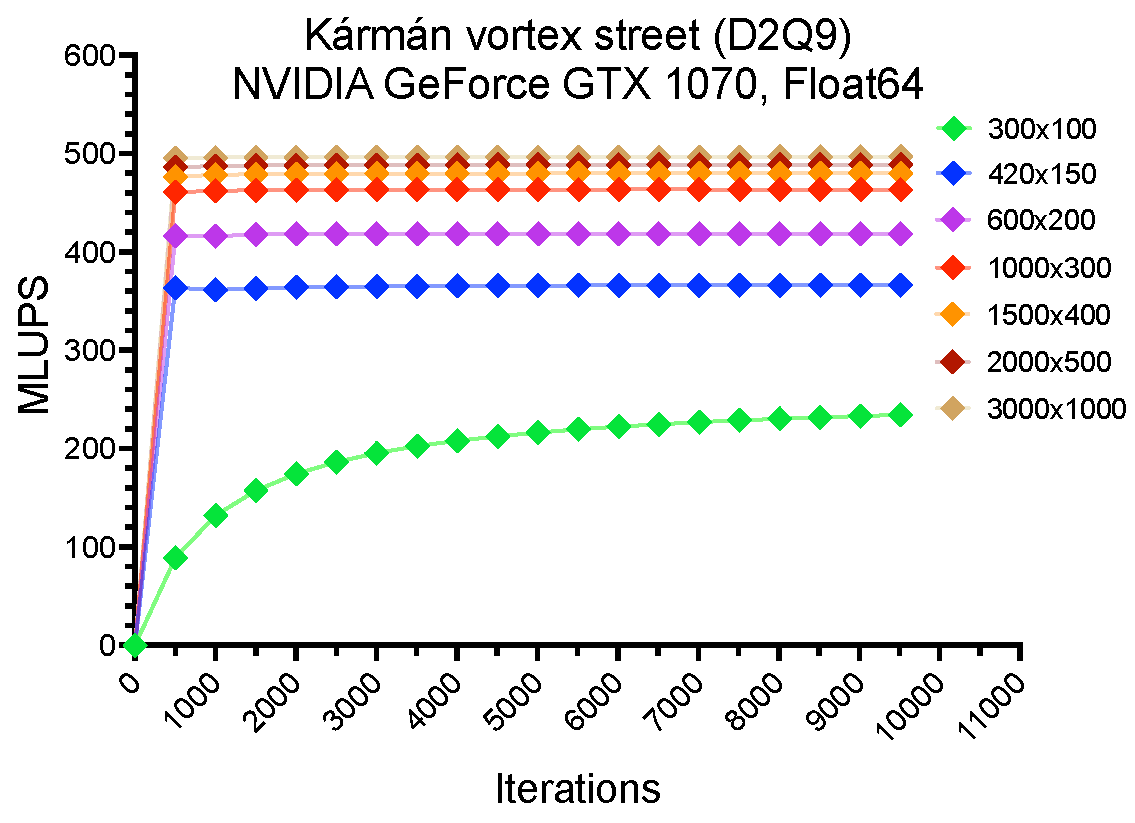
\includegraphics[width=0.45\textwidth]{data/gtx1070_64bit_d2q9_bgk_channel_mlups.pdf}%
	}\qquad
	\subfloat[Performance on RTX 2080 Ti GPU.\label{fig:d2q9_channel_mlups_rtx2080ti_64bit}]{%
		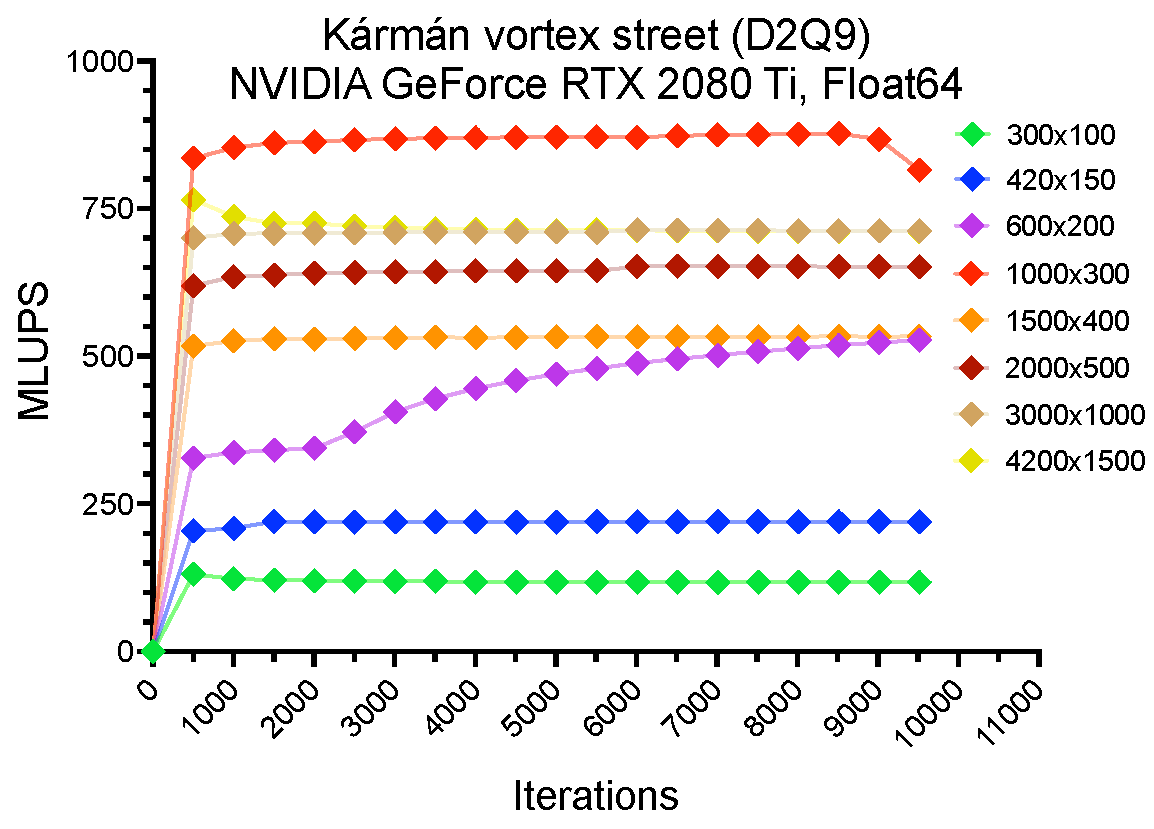
\includegraphics[width=0.45\textwidth]{data/rtx2080ti_64bit_d2q9_bgk_channel_mlups.pdf}%
	}\qquad
	\subfloat[Performance on RTX 3090 GPU.\label{fig:d2q9_channel_mlup_rtx3090_64bit}]{%
		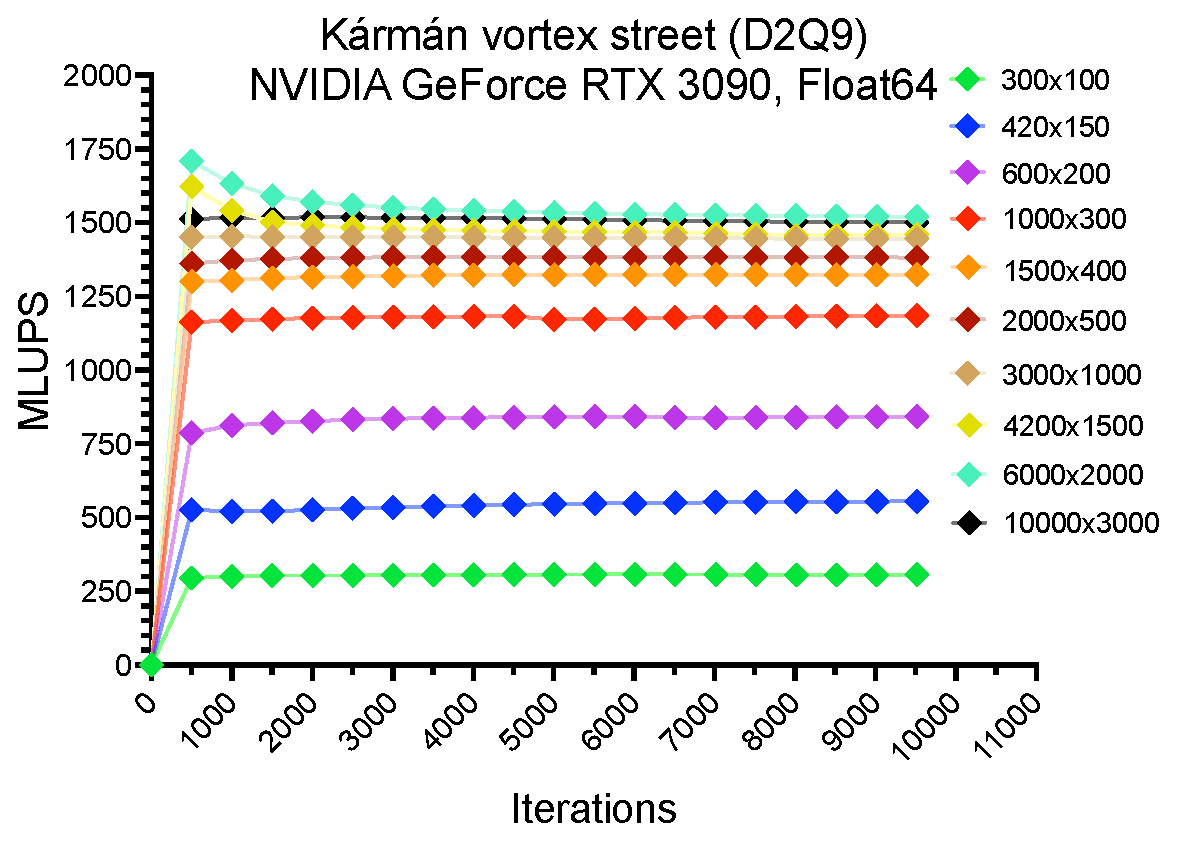
\includegraphics[width=0.45\textwidth]{data/rtx3090_64bit_d2q9_bgk_channel_mlups.pdf}%
	}
	\captionsetup{justification=centering}
	\caption{Double-precision performance analysis of 2D Kármán vortex on D2Q9 stencil.}
	\label{fig:d2q9_channel_mlups_f64}
\end{figure}

Maximum MLUPS of the GPUs for single-precision calculations for 2D test cases are slightly higher than the study reported by Boroni et. al \cite{FULLGPUImplementation2017}, in which they reported 80 MLUPS at peak performance achieved on NVIDIA GeForce GTX 580 GPU. The AMD Radeon R9 M370X GPU used in our work can be seen as similarly performing card. 

\begin{figure}[!ht]
	\centering
	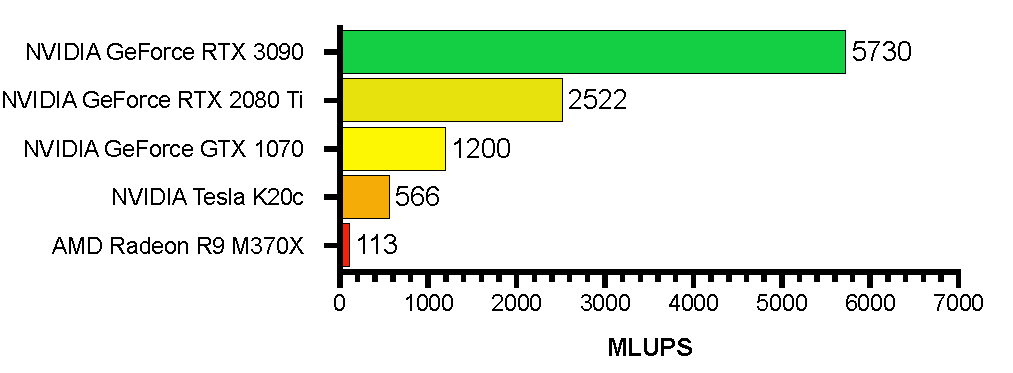
\includegraphics[width=0.8\textwidth]{data/max_mlups_2d.pdf}
	\caption{Peak performance of single-precision LBM simulations on D2Q9 stencil.}
	\label{fig:max_mlups}
\end{figure}

For the 3D LBM simulation with D3Q27 stencil and multiple-relaxation time (MRT), results showed the computation speeds reaching up to 1500 MLUPS in single-precision (Figure~\ref{fig:d3q27_lid_mlups_f32}) and up to 490 MLUPS in double-precision benchmarks Figure~\ref{fig:d3q27_lid_mlups_f64}. The MRT is much more computationally intensive than BGK and with the 27 particle distributions to track, the difference between D2Q9 and D3Q27 is significant. The memory bandwidth for D3Q27 lid-driven cavity tests is much higher, therefore we were limited to grids under $128^3$ in current implementation.

In 3D lid-driven cavity test, benchmarks showed inconsistencies with expectations and actual results (Table \ref{tab:lid-mlups-all-3d}). The performance is lower in coarse grids ($16^3$ and $32^3$) with more powerful RTX 2080 Ti conversely to higher performance reported with weaker GTX 1070 (Figure~\ref{fig:d3q27_lid_mlups_gtx1070_32bit} and Figure~\ref{fig:d3q27_lid_mlups_rtx2080ti_32bit}). This points to the well-known problem of representing multi-dimensional data in the most optimal way stop GPU from cache misses. It means the data organization of 27 individual distribution functions in D3Q27 lattice nodes along 3D grid has to be rethought and reimplemented to address this issue.  

\begin{table}[!ht]
	\centering\small
	{\renewcommand{\arraystretch}{1.1}%
		{\setlength{\tabcolsep}{0.5em}
	\begin{tabular}{ |p{3.2cm}||p{2.2cm}|p{2.2cm}|p{2.4cm}|p{2.2cm}|  }
		\hline
		Domain & R9 M370X & GTX~1070 & RTX~2080~Ti & RTX 3090 \\
		\hline
		16$\times$16$\times$16   & 7 & 25  & 28  & 40  \\
		\hline
		32$\times$32$\times$32   & 18 & 155  & 70   & 225  \\
		\hline
		64$\times$64$\times$64   & 97 & 675  & 186   & 868  \\
		\hline
		128$\times$128$\times$128   & 120 & 1006  & 600   & 2890  \\
		\hline
	\end{tabular}}}
	\caption{Peak MLUPS of lid-driven cavity test case in 3D. The data represents single-precision floating point computation (taking only the steady performance after initial warm-up and removal of sudden spikes).}
	\label{tab:lid-mlups-all-3d}
\end{table}

\begin{figure}[!ht]
	\centering
	\subfloat[Performance on Radeon R9 M370X GPU.\label{fig:d3q27_lid_mlups_r9_32bit}]{%
		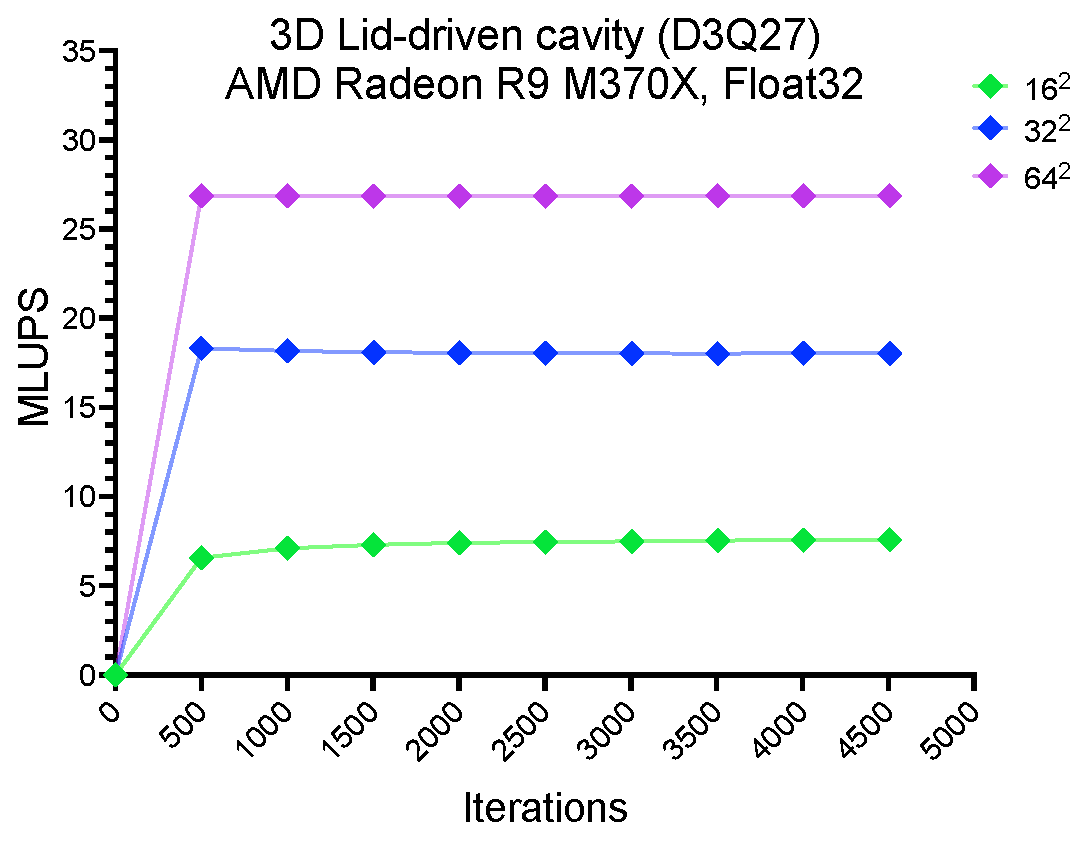
\includegraphics[width=0.45\textwidth]{data/r9_32bit_d3q27_mrt_lid_mlups.pdf}%
	}\qquad
	\subfloat[Performance on GTX 1070 GPU.\label{fig:d3q27_lid_mlups_gtx1070_32bit}]{%
		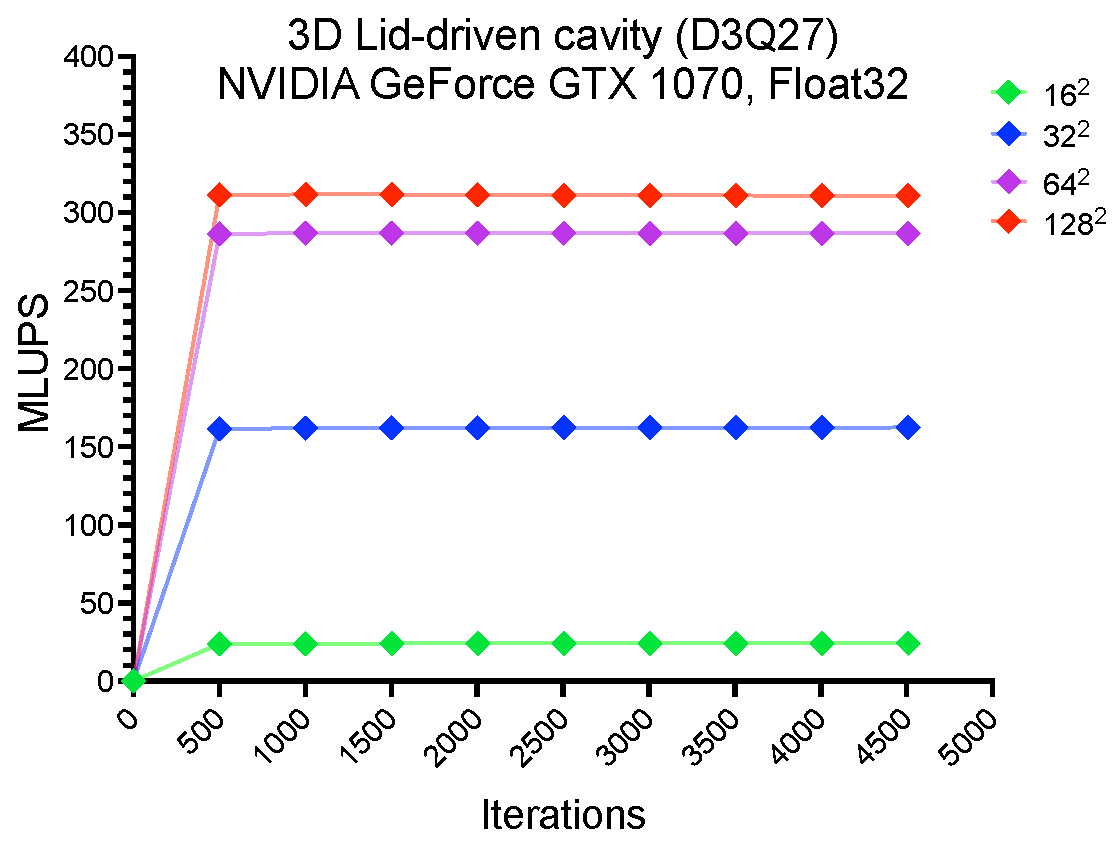
\includegraphics[width=0.45\textwidth]{data/gtx1070_32bit_d3q27_mrt_lid_mlups.pdf}%
	}\qquad
	\subfloat[Performance on RTX 2080 Ti GPU.\label{fig:d3q27_lid_mlups_rtx2080ti_32bit}]{%
		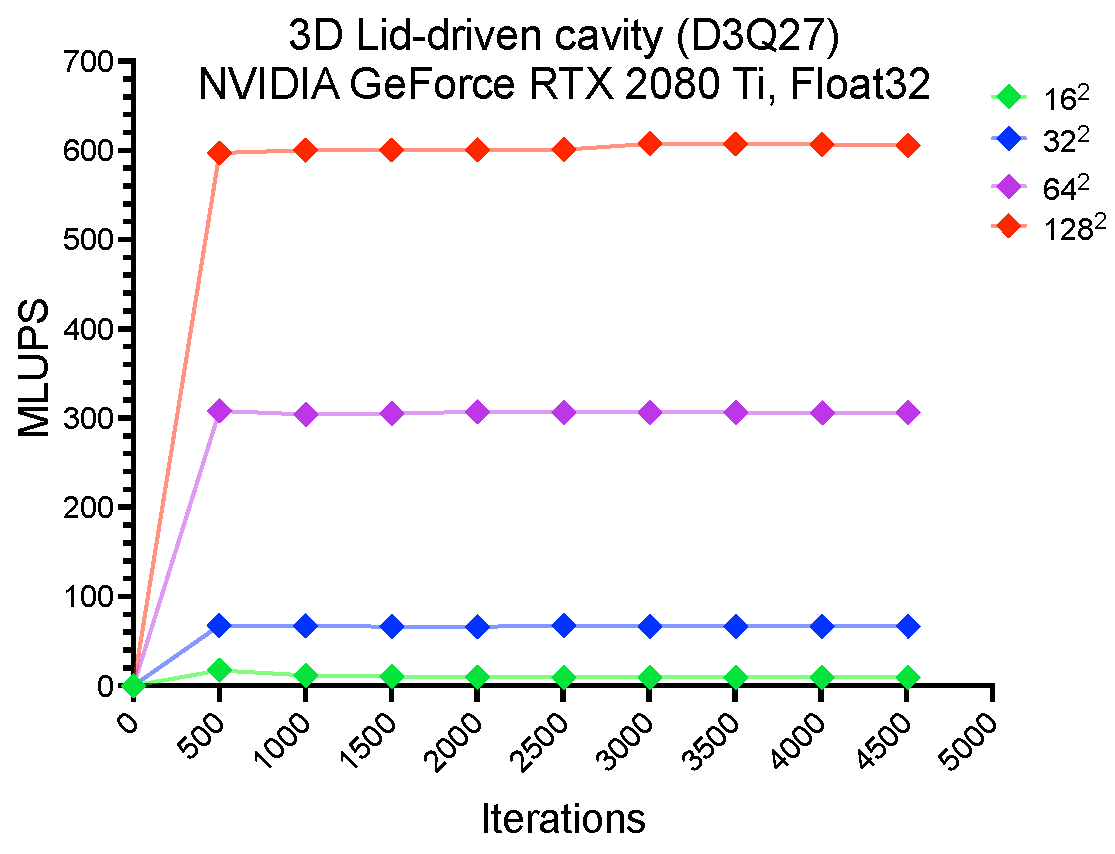
\includegraphics[width=0.45\textwidth]{data/rtx2080ti_32bit_d3q27_mrt_lid_mlups.pdf}%
	}\qquad
	\subfloat[Performance on RTX 3090 GPU.\label{fig:d3q27_lid_mlups_rtx3090_32bit}]{%
		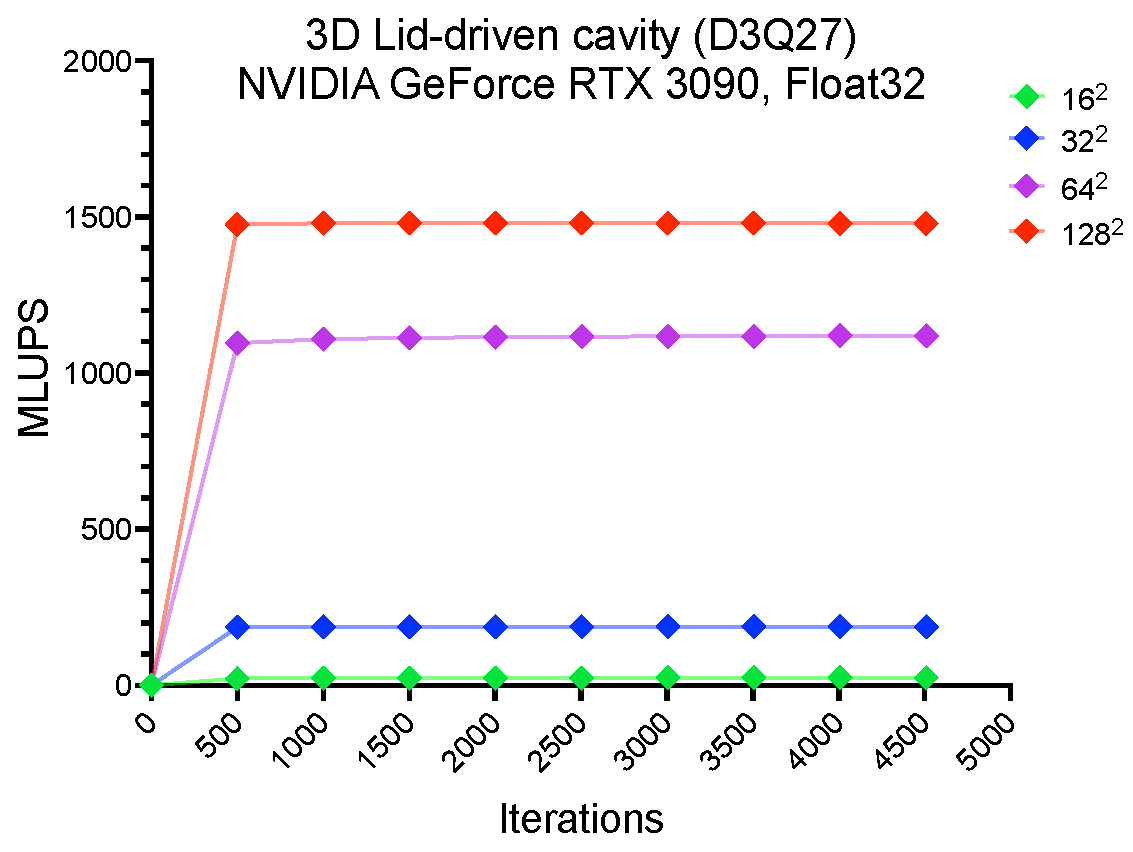
\includegraphics[width=0.45\textwidth]{data/rtx3090_32bit_d3q27_mrt_lid_mlups.pdf}%
	}
	\captionsetup{justification=centering}
	\caption{Single-precision performance analysis of 3D lid-driven cavity on D3Q27 stencil with multiple-relaxation time.}
	\label{fig:d3q27_lid_mlups_f32}
\end{figure}

\begin{figure}[!ht]
	\centering
	\subfloat[Performance on Radeon R9 M370X GPU.\label{fig:d3q27_lid_mlups_r9_64bit}]{%
		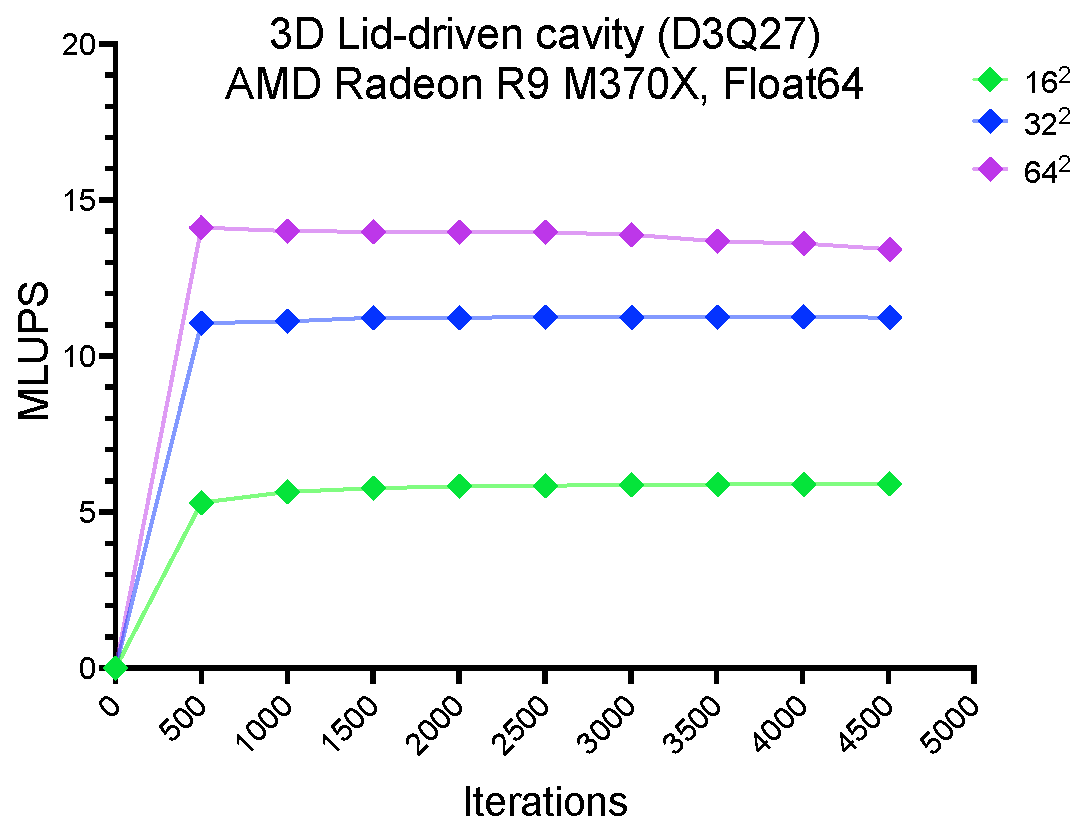
\includegraphics[width=0.45\textwidth]{data/r9_64bit_d3q27_mrt_lid_mlups.pdf}%
	}\qquad
	\subfloat[Performance on GTX 1070 GPU.\label{fig:d3q27_lid_mlups_gtx1070_64bit}]{%
		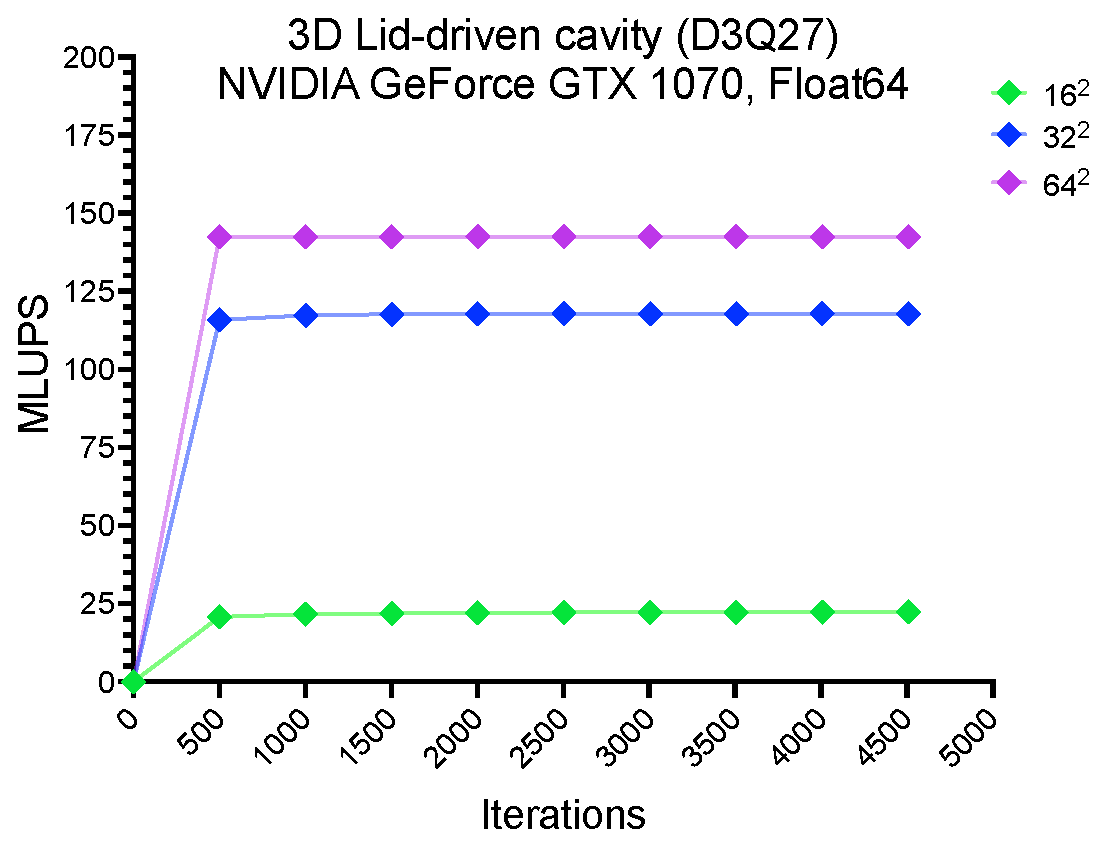
\includegraphics[width=0.45\textwidth]{data/gtx1070_64bit_d3q27_mrt_lid_mlups.pdf}%
	}\qquad
	\subfloat[Performance on RTX 2080 Ti GPU.\label{fig:d3q27_lid_mlups_rtx2080ti_64bit}]{%
		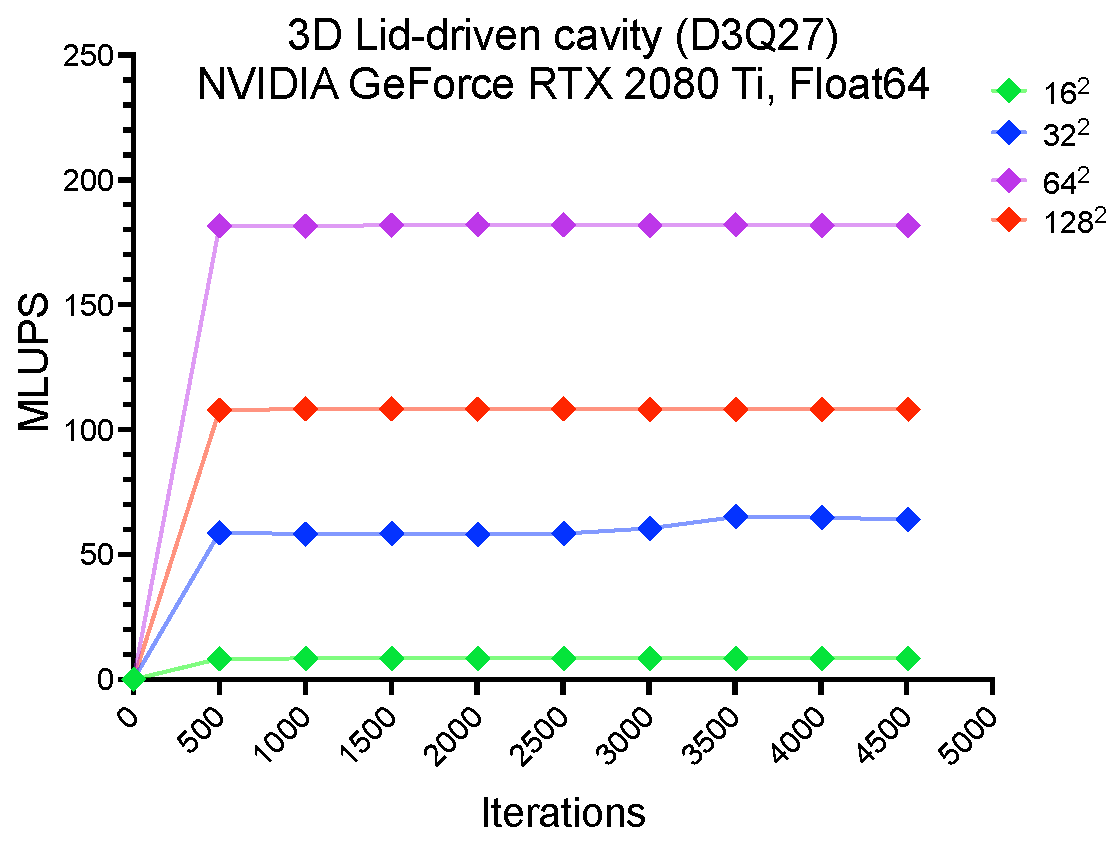
\includegraphics[width=0.45\textwidth]{data/rtx2080ti_64bit_d3q27_mrt_lid_mlups.pdf}%
	}\qquad
	\subfloat[Performance on RTX 3090 GPU.\label{fig:d3q27_lid_mlups_rtx3090_64bit}]{%
		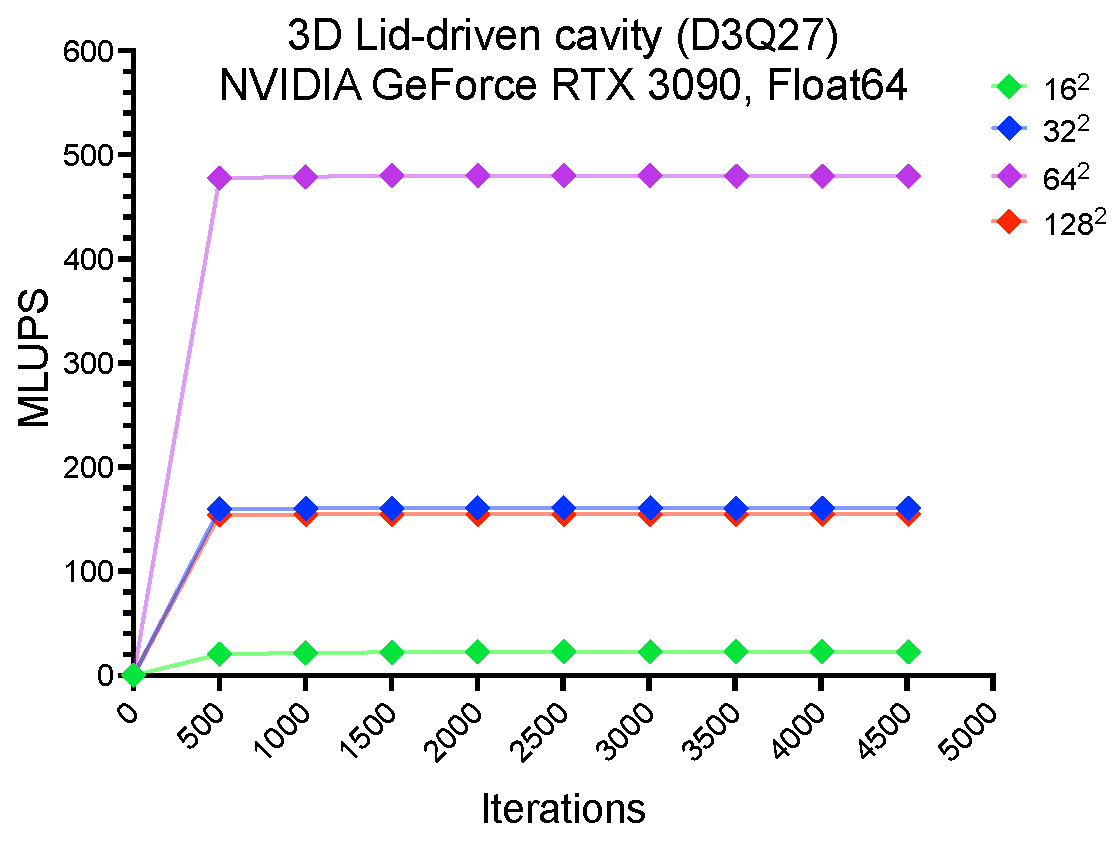
\includegraphics[width=0.45\textwidth]{data/rtx3090_64bit_d3q27_mrt_lid_mlups.pdf}%
	}
	\captionsetup{justification=centering}
	\caption{Double-precision performance analysis of 3D lid-driven cavity on D3Q27 stencil with multiple-relaxation time..}
	\label{fig:d3q27_lid_mlups_f64}
\end{figure}

When comparing the 3D performance of LBM solvers, and specifically those using D3Q27 stencil with multiple-relaxation times, our LBM-MRT solver has still lot of room for improvement. One of the fastest solvers on the market for such 3D LBM smulation is Sailfish \cite{januszewskiSailfishFlexibleMultiGPU2014}. They take advantage of multi-GPU and many-core CPU support in their software, but even for single-GPU, our solver doesn't reach the satisfactory speeds comparable to Sailfish. In D3Q27 solver described in this work, maximum MLUPS achieved for single-precision calculations in 3D test cases on similar hardware is shown in Figure~\ref{fig:max_mlups_3d}. 

\begin{figure}[!ht]
	\centering
	\includegraphics[width=0.8\textwidth]{data/max_mlups_3d.pdf}
	\caption{Peak performance of single-precision LBM simulations on D3Q27 stencil with multiple-relaxation time.}
	\label{fig:max_mlups_3d}
\end{figure}

\section{Conclusions}

For this thesis, the cross-platform LBM solver that can be used on variety of parallel accelerators (e.g. GPUs, CPUs or FPGAs) was implemented. It uses ArrayFire, a high-performance parallel computing library (version 3.8.0 was used for this work). We created reference implementation in C++ and ported the same code to Rust. We chose Rust because it has modern capabilities, is memory safe and its performance is comparable to C/C++. We were able to produce sufficient LBM solver in under 150 lines of code, including real-time visualization code. Benchmarks were concluded for both C++ and Rust versions, resulting in identical performance. Data reported in this study are taken from the Rust version. 

For the benchmarks, we analyzed two classical, academic test cases, the lid-driven cavity and Kármán vortex street (flow around the obstacle in pipe). We employed commonly used metric for measuring speed of LBM implementations, the MLUPS. We benchmarked our LBM implementation on 5 different GPUs and one CPU. Between CPU and GPU, we saw from 4 to more than 300 times speedup on various GPUs.

\section{Discussion}

\subsection{Future Work}

As with work such as these

\subsubsection{Application to Real World}

Biology \\
Steelmaking \\
Non-newtonian fluids \\

%https://en.wikipedia.org/wiki/Fluid_mechanics#Newtonian_versus_non-Newtonian_fluids


%A Newtonian fluid (named after Isaac Newton) is defined to be a fluid whose shear stress is linearly proportional to the velocity gradient in the direction perpendicular to the plane of shear. This definition means regardless of the forces acting on a fluid, it continues to flow. For example, water is a Newtonian fluid, because it continues to display fluid properties no matter how much it is stirred or mixed. A slightly less rigorous definition is that the drag of a small object being moved slowly through the fluid is proportional to the force applied to the object. (Compare friction). Important fluids, like water as well as most gases, behave—to good approximation—as a Newtonian fluid under normal conditions on Earth.
%
%Describe non-Newtonian fluids found in steelmaking processes...

\subsubsection{Streaming Visualized Pixels Over Network}

\subsubsection{Simulation as an Educational Tool}
%
%In some simplified form, combinations of numerical simulations and visualizations of steel- making processes can be used as a educational tool in process control courses at technical universities. The aim of the online, web-based interactive simulation of basic oxygen steelmaking at steeluniversity.org shown in Figure~ \ref{fig:steeluniversity} is to introduce students to this process in a more fun and engaging way.
%
%\begin{figure}[!ht]
%	\label{fig:steeluniversity}
%	\centering
%	\includegraphics[width=0.8\textwidth]{figures/steeluniversity.jpg}
%	\caption{Interactive, educational simulation of basic oxygen steelmaking by steeluniversity.org.}
%\end{figure}


% USE AT YOUR OWN RISK

%\section{Basic Oxygen Furnace (BOF)}
%
%The oxygen converter process (LD/BOF and its derivatives) is a refinement step in the production of steel from ore. The main purpose of the process is to remove excess carbon from the pig iron produced in the blast furnace. The main feature of the process is to add oxygen through a top lance, in order to remove unwanted impurities through oxidation. It is the main method of carbon and low alloy steelmaking, annual production approaching to 60\% of total crude steel production \cite{Jalkanen2006}. BOF is a widely preferred and effective steelmaking method due to its high productivity and considerably low production cost \cite{Wang2010}. LD/BOF process consists of these subprocesses:
%
%\begin{enumerate}
%	\item Charging slag
%	\item Charging hot metal
%	\item Oxygen blowing and addition of slagging and alloying additives 4. Measurement of steel temperature and composition
%	\item Tapping of steel
%	\item Tapping of slag
%\end{enumerate}
%
%The first commercial operation of steelmaking with oxygen top blowing in the converter was in the early 1950s at Linz and Donawitz (Austria). This manner of steelmaking became known as Linz-Donawitz or LD process. For many years now, most of the steel has been made by top oxygen blowing for which different names are given. For example, in European steel plants the process is still called LD; in the UK, BOS (basic oxygen steel- making); in the Far East and America, BOF (basic oxygen furnace), with the exception of U.S. Steel where it is called basic oxygen process \cite{Turkdogan1996}.
%
%\begin{figure}[!ht]
%	\label{fig:bof-single}
%	\centering
%	\includegraphics[width=0.5\textwidth]{figures/bof-single.jpg}
%	\caption{Production of steel in the converter with top-blown oxygen (LD/BOF) \citep{Turkdogan1996}.}
%\end{figure}
%
%In modern steel mills about 300 tons of steel are produced within a 30-40 minute cycle. Various additives are added during the process to adapt the steel quality and slag formation. The converter furnace is inclined during charging and tapping. The converter has a vertical position during oxygen blowing. The changes in the position of the converter during the individual elementary processes are shown in the figure \ref{fig:convertor-phases}.
%
%
%\begin{figure}[!ht]
%	\label{fig:convertor-phases}
%	\centering
%	\includegraphics[width=0.4\textwidth]{figures/convertor-phases.jpg}
%	\caption{Representation of elementary processes in LD converter.}
%\end{figure}
%
%Depending on local operating conditions, availability of scrap, blast furnace iron and the extent of hot metal pretreatment, the metallic charge (LD/BOF, Q-BOP) is $75$ to $95\%$ pig iron and the remainder is steel scrap. The types of scrap used are usually those produced in a steel mill: sheet scrap, damaged molds, bimetallic cans etc. \citep{Turkdogan1996}.
%
%Oxygen is blown at a high speed (up to twice the speed of sound) on the surface of the metal bath in the converter and so-called hot area is formed in the region where the oxygen stream hits the surface. The oxidation products dissolve in the slag, with the exception of carbon monoxide, which passes through the slag layer and forms the major component of the converted gas. The oxidation intensity of the individual elements depends on their chemical affinity for oxygen. Carbon oxidation is one of the most important processes. Carbon is oxidized in the metal during the steelmaking process by the influence of oxygen, in particular on \ce{CO} and partly on \ce{CO2}, depending on the reactions
%
%\begin{equation}
%	\ce{ C + 1/2 O2 -> 2CO }
%\end{equation}
%
%\begin{equation}
%	\ce{ C + O2 -> CO2 }
%\end{equation}
%
%Manganese is oxidized to \ce{MnO}
%
%\begin{equation}
%	\ce{ Mn + 1/2 O2 -> MnO },
%\end{equation}
%
%Phosphorus is undesirable in steel and oxidizes to \ce{P2O5}
%
%\begin{equation}
%	\ce{ 2P + 5/2 O2 -> P2O5 }.
%\end{equation}
%
%Sulphur is a harmful element and passes into the slag in the form of \ce{CaS} based on the reaction of \ce{CaO}
%
%\begin{equation}
%	\ce{ CaO + MnS -> CaS + MnO }
%\end{equation}
%
%whereby \ce{MnS} is formed by reaction
%
%\begin{equation}
%	\ce{ Mn + S -> MnS }
%\end{equation}
%
%and sulphur also goes out in the form of gas as \ce{SO2}
%
%\begin{equation}
%	\ce{ S + O2 -> SO2 }.
%\end{equation}
%
%Silicon has a high affinity for oxygen, so it is easily oxidized to form \ce{SiO2}
%
%\begin{equation}
%	\ce{ Si + O2 -> SiO2 }.
%\end{equation}
%
%In the initial stages of blowing, most of the silicon oxidizes to form a slag of low basicity - the composition of the metal and slag changes TODO: DOPLNIT ZDROJ!!!. 
%
%An intense oxygen flow induces fluid flows in the iron bath, forcing the highly oxidized metal and the molten oxidation products from the iron bath surface to penetrate into the bath, where they react with the ``fresh" hot metal with a high content of impurities and therefore loss of iron in the form of \ce{FeO} and \ce{Fe2O3}should also be considered:
%
%\begin{equation}
%	\ce{ Fe + 1/2 O2 -> FeO }
%\end{equation}
%
%\begin{equation}
%	\ce{ 2Fe + 3/2 O2 -> Fe2O3 }.
%\end{equation}
%
%This oxygen stream and gas bubbles generated in the bath bring portions of the iron melt to the slag. The heat generated by the highly exothermic oxidation reactions is consumed by heating and melting the feed materials, heating the iron bath, slag and carbon oxides that are formed during the oxidation of the carbon and are partially lost to the environment during the blowing process.
%
%The resulting \ce{SiO2} passes into the slag as \ce{2CaO.SiO2} according to the equation
%
%\begin{equation}
%	\ce{ SiO2 + 2CaO -> 2CaO.SiO2 }
%\end{equation}
%
%and additionally, \ce{P2O5} passes into the slag as \ce{3CaO.P2O5} according to the equation \cite{sprava2017}
%
%\begin{equation}
%	\ce{ P2O5 + 3CaO = 3CaO.P2O5 }
%\end{equation}
%
%Circulation in the iron bath caused by the flow of oxygen, rising gas bubbles and purging of inert gas through the lower tubes in converters with combined blowing type transports minor iron melt components (C, Si, Ti, Mn, P, V, etc.) to the upper bath layers \citep{Jalkanen2006}.
%
%\begin{figure}[!ht]
%	\label{fig:ld-convertor-processes-graphical}
%	\centering
%	\includegraphics[width=0.8\textwidth]{figures/ld-convertor-processes-graphical.jpg}
%	\caption{Chemical and thermal processes in LD converter \citep{Jalkanen2006}.}
%\end{figure}
%
%\subsubsection{Chemical Kinetics}
%
%- TODO: Citovanie z monografie "Modelovanie a optimalne riadenie KP"
%
%Chemical kinetics is the study of homogenous and heterogeneous chemical reactions and phase changes. In BOF 
%
%\subsubsection{Control of Production Processes in BOF}
%
%In order to monitor and control the process, different measuring systems can be employed to give feedback to either the operator or directly to existing system for automated control. These measurements can be either direct or indirect as well as with or without time delays. The real-time information on the process state can be obtained from a number of sensors, e.g. off-gas flow rate from venturi; off-gas temperature with temperature sensors; indication of changes in slag level from sound level measurement with microphone, accelerometer on lance or vessel or lance elongation sensor; pressure difference with ambient pressure with hood pressure sensor, etc.
%
%All these signals can, in principle, be used for closed-loop control. Changes in lance height are easier to measure as well as set and therefore preferable to use in a closed- loop control system. Oxygen gas flow rate should not be changed more than approximately $\pm5\%$ since the nozzle is designed for a specific flow rate \citep{Widlund1998}.
%
%TODO: DOPLNIT SCHEMU RIADIACEHO SYSTEMU
%
%Different operators apply different rules for deciding when to stop the blowing of oxygen. These operator induced irregularities make it difficult to achieve production disturbances. The converter process is only one link in a chain of unit operations from raw materials to final product. Therefore, production disturbances can change process conditions. For example, poor blast furnace performance might lead to insufficient hot metal supply or even production disruptions. Under these circumstances, more metal scrap and fuel should be used instead of hot metal to uphold production volumes. Logically, this implies changes in blowing practice \citep{Widlund1998}.